%% The "\appendix" call has already been made in the declaration
%% of the "appendices" environment (see thesis.tex).
\chapter{Appendices}
\label{app:appendices}

\section{Characterisation of the signal and control regions}
\label{app:charac}

Extra data-\MC comparisons of the key analysis variables in each of
the signal and control regions of the analysis are included in this
section

% \clearpage
% \subsection{Yields and distributions for the muon + jets control sample}

\begin{figure}
    \begin{center}
        \subfloat {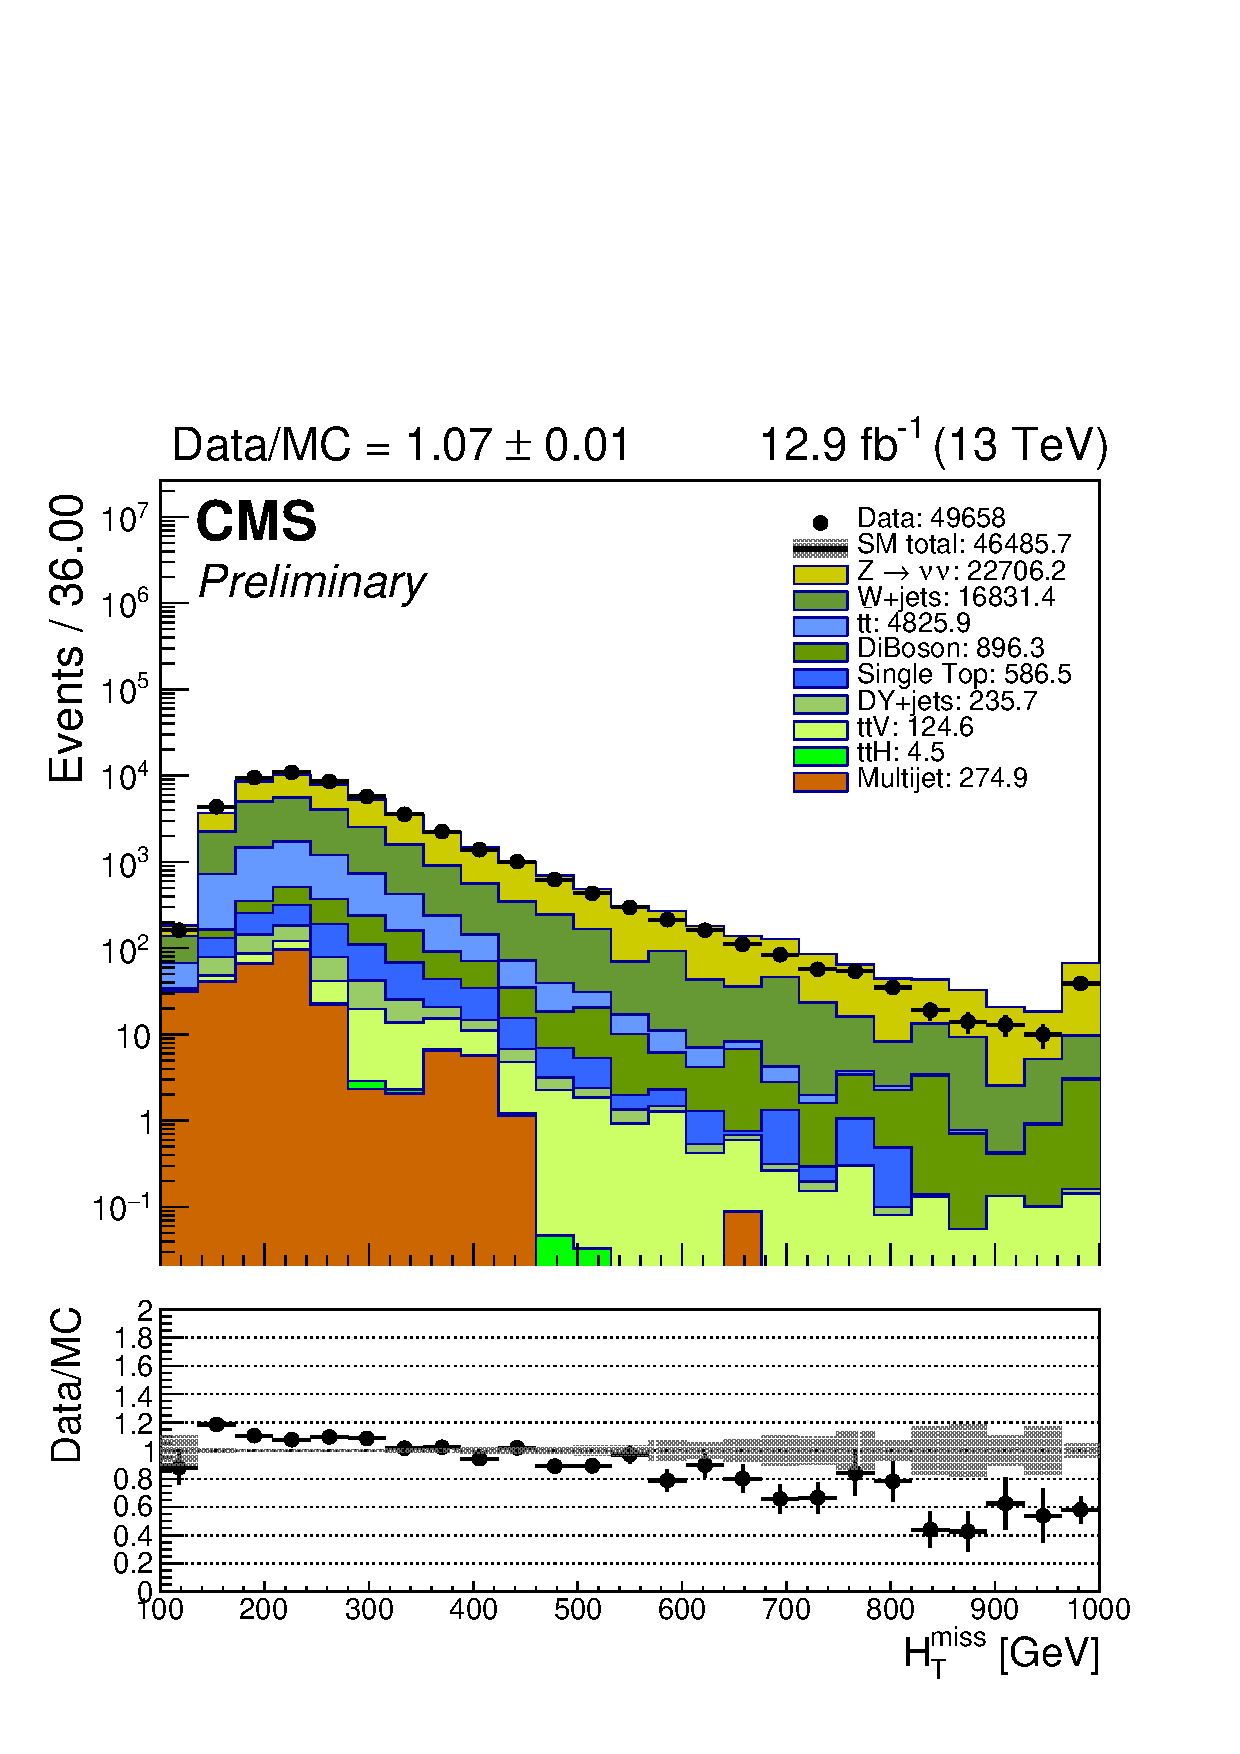
\includegraphics[width=0.5\textwidth]{figs/analysis/distributions/Signal/mht40_pt_sym.pdf}} ~~
        \subfloat {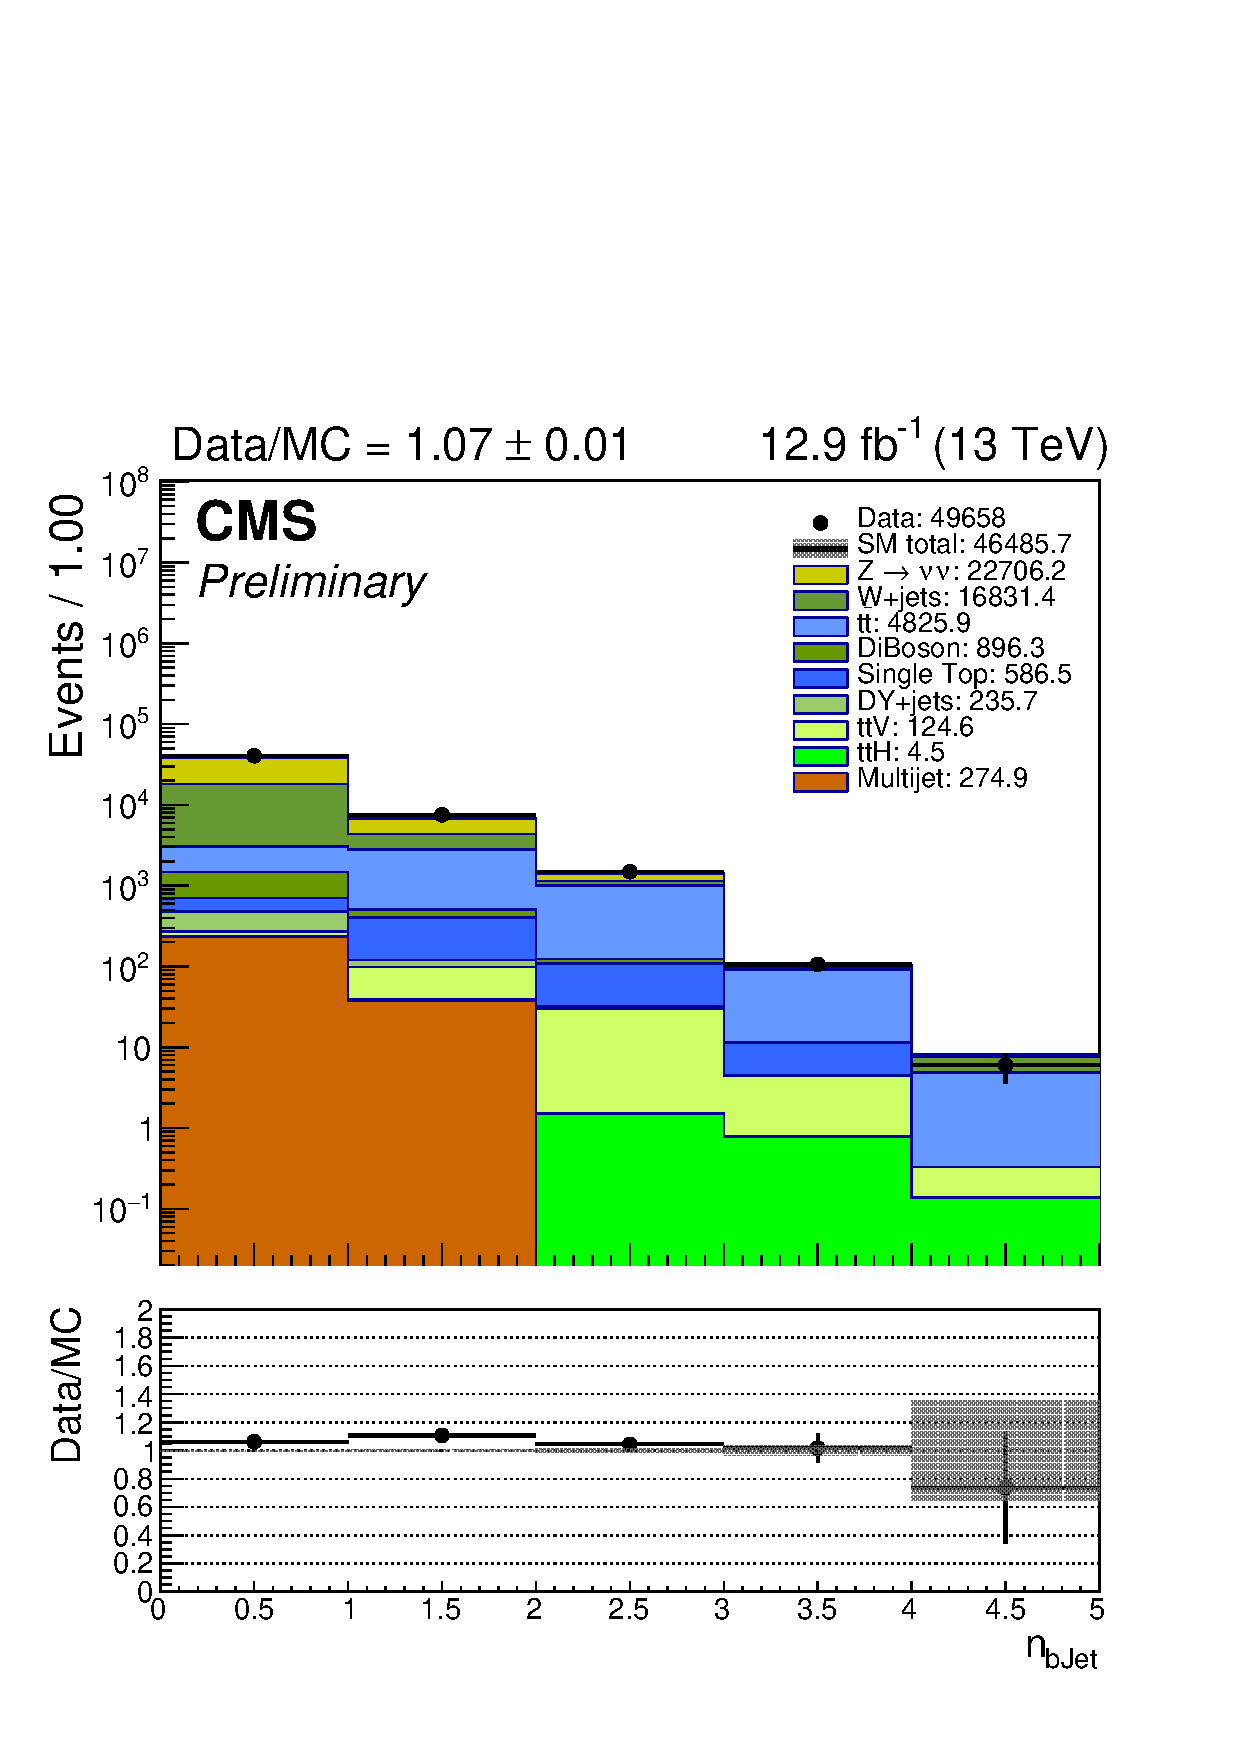
\includegraphics[width=0.5\textwidth]{figs/analysis/distributions/Signal/nBJet40_sym.pdf}} \\
        \caption{Key analysis variables for hadronic signal region (symmetric \njet bins)}
        \label{fig:distribution_signal_sym}
    \end{center}
\end{figure}

\clearpage
\begin{figure}
    \begin{center}
        \subfloat {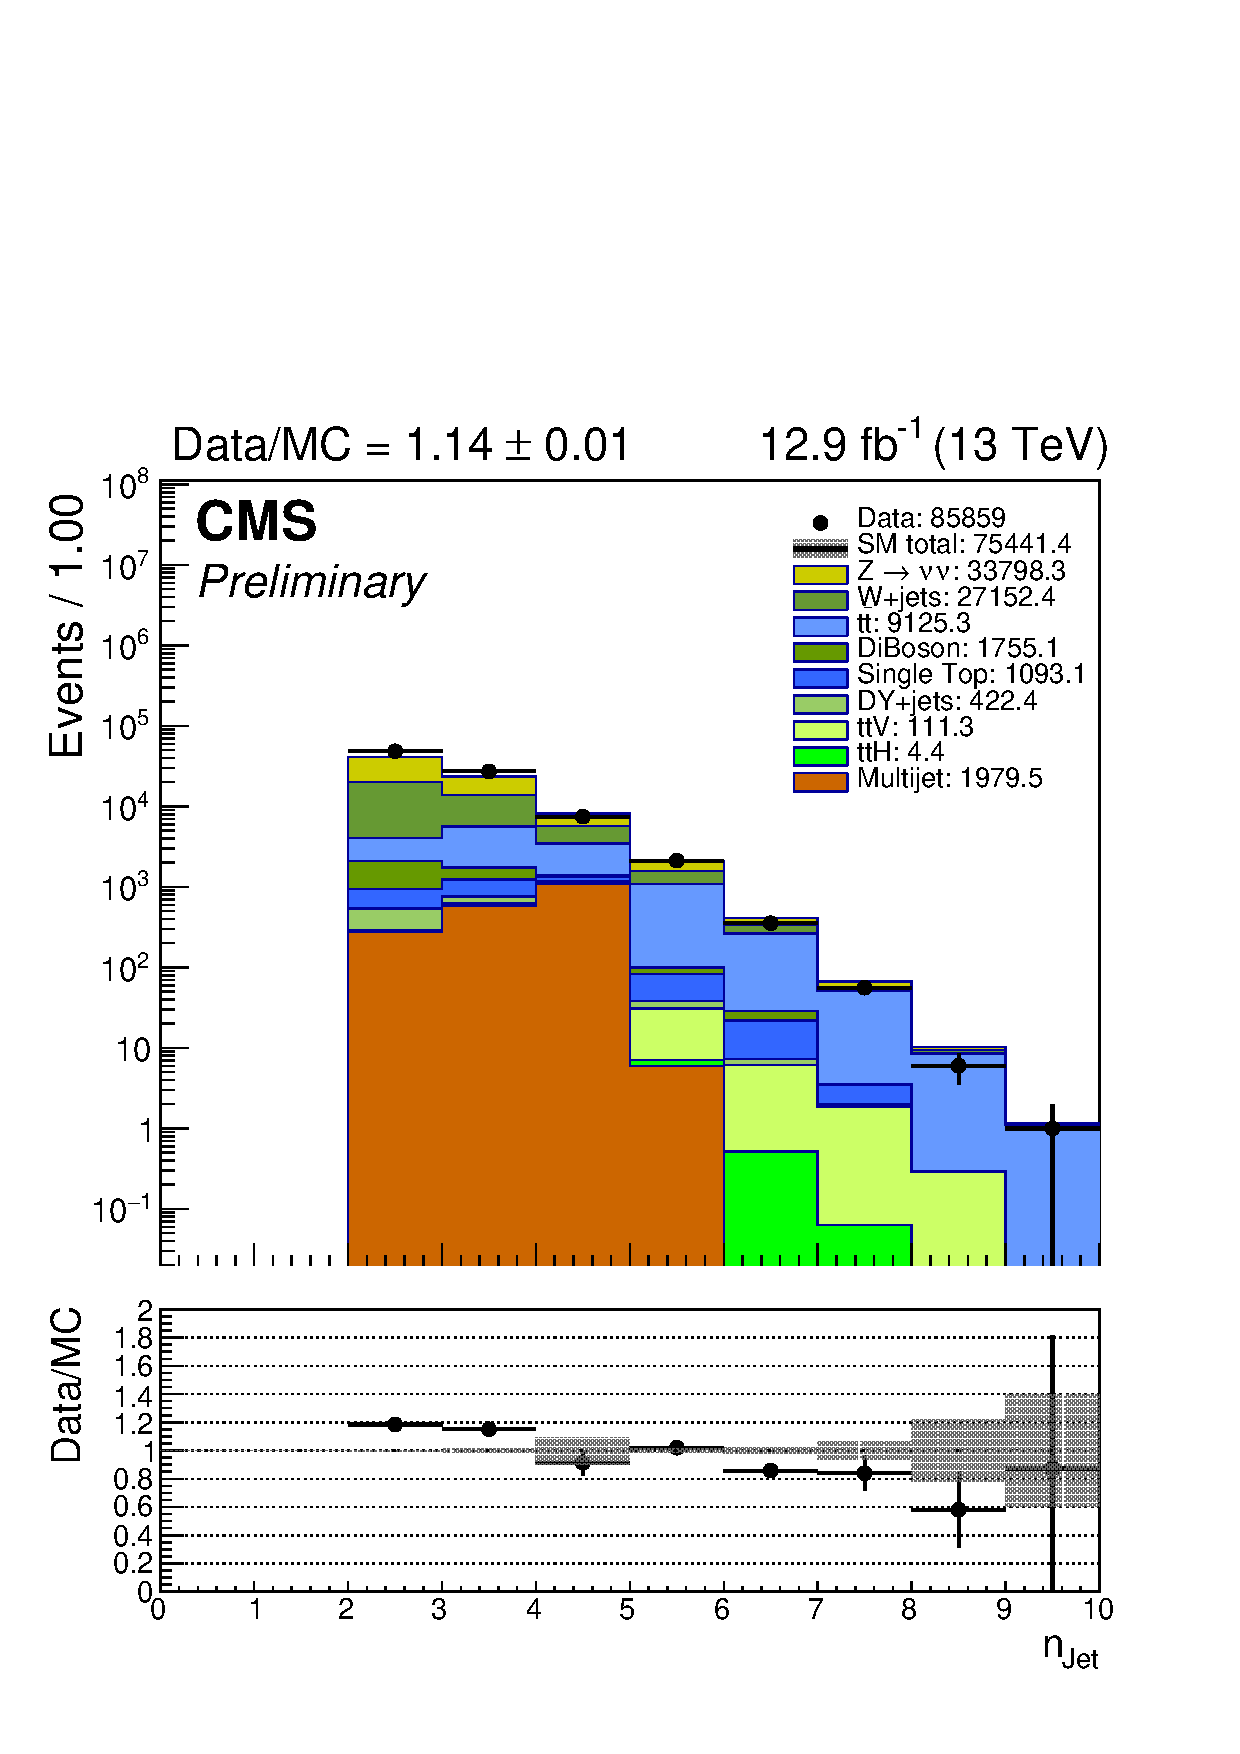
\includegraphics[width=0.5\textwidth]{figs/analysis/distributions/Signal/nJet40_asym.pdf}} ~~
        \subfloat {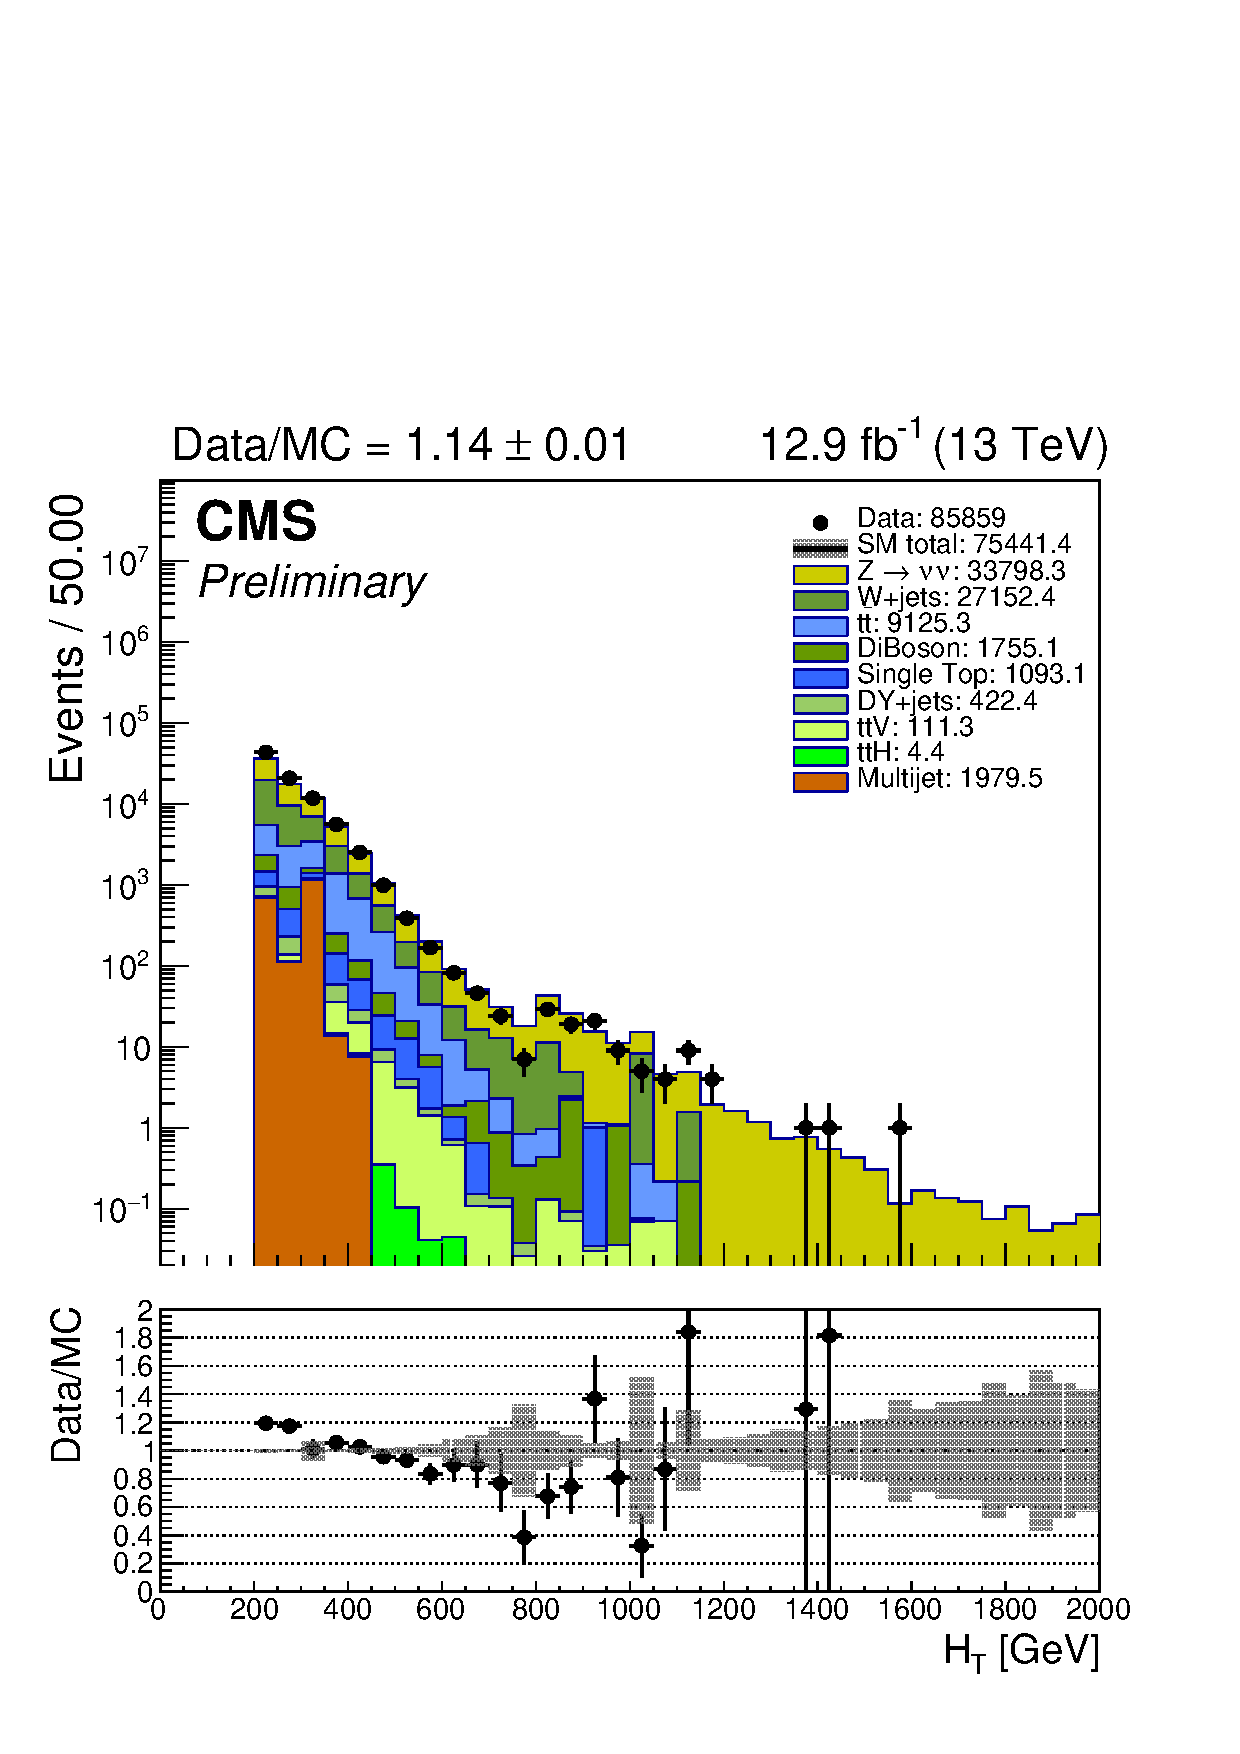
\includegraphics[width=0.5\textwidth]{figs/analysis/distributions/Signal/ht40_asym.pdf}} \\
        \subfloat {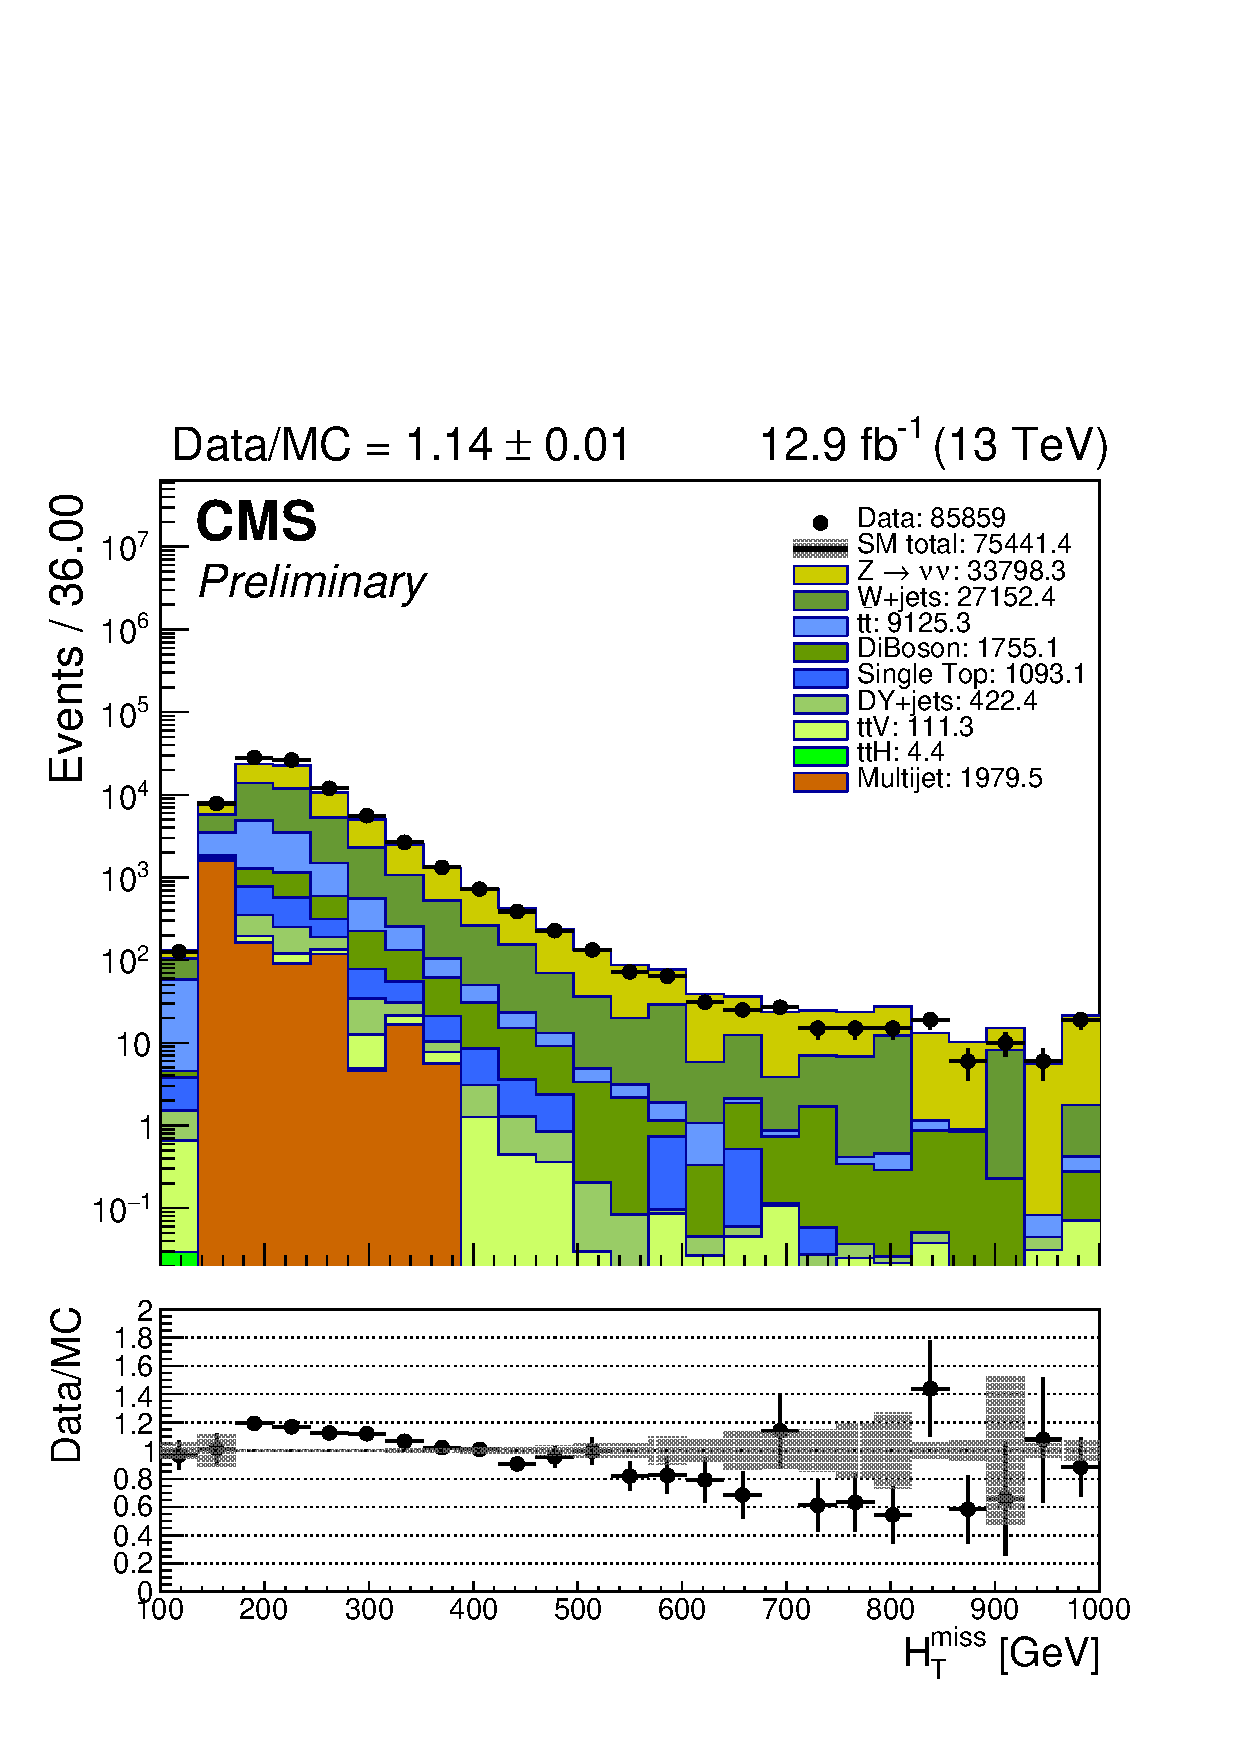
\includegraphics[width=0.5\textwidth]{figs/analysis/distributions/Signal/mht40_pt_asym.pdf}} ~~
        \subfloat {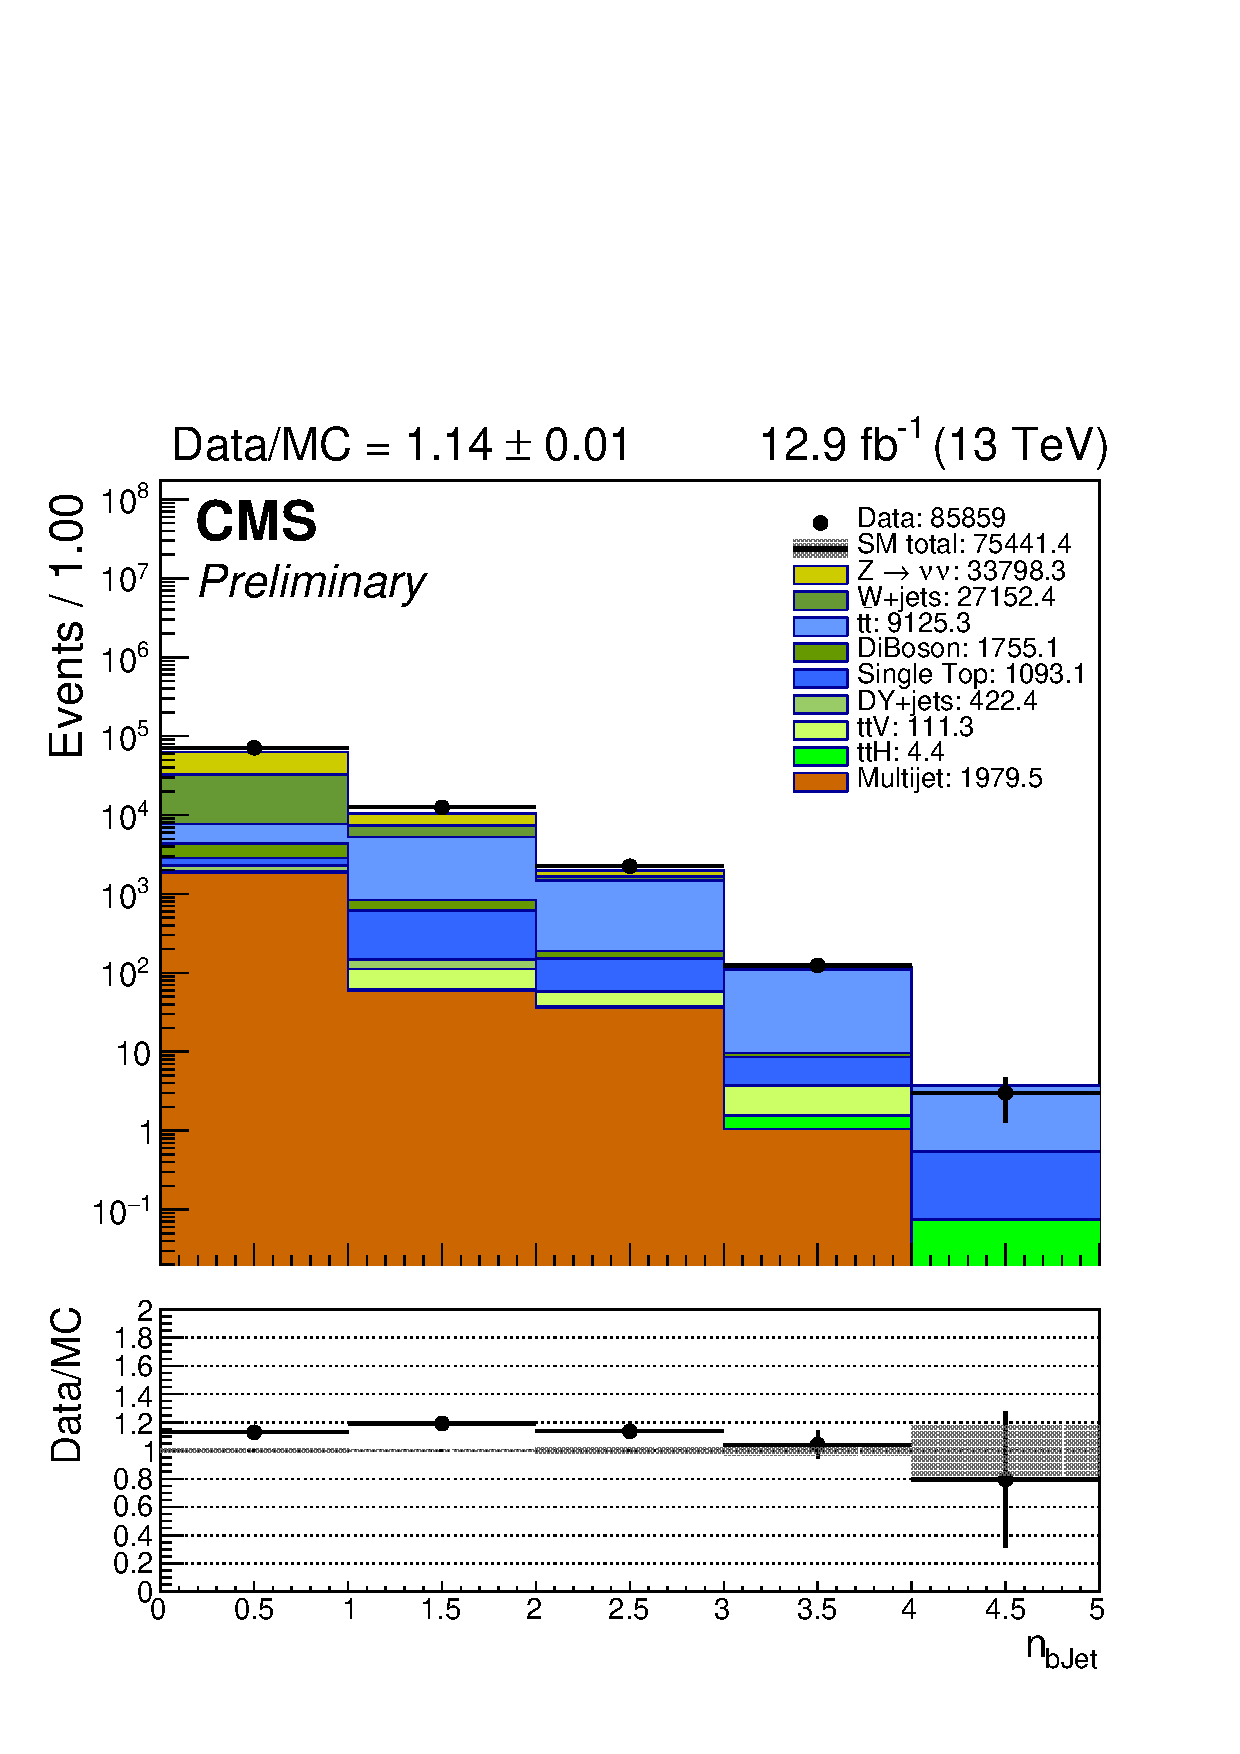
\includegraphics[width=0.5\textwidth]{figs/analysis/distributions/Signal/nBJet40_asym.pdf}} \\
        \caption{Key analysis variables for hadronic signal region (asymmetric \njet bins)}
        \label{fig:distribution_signal_asym}
    \end{center}
\end{figure}

\clearpage
\begin{figure}
    \begin{center}
        \subfloat {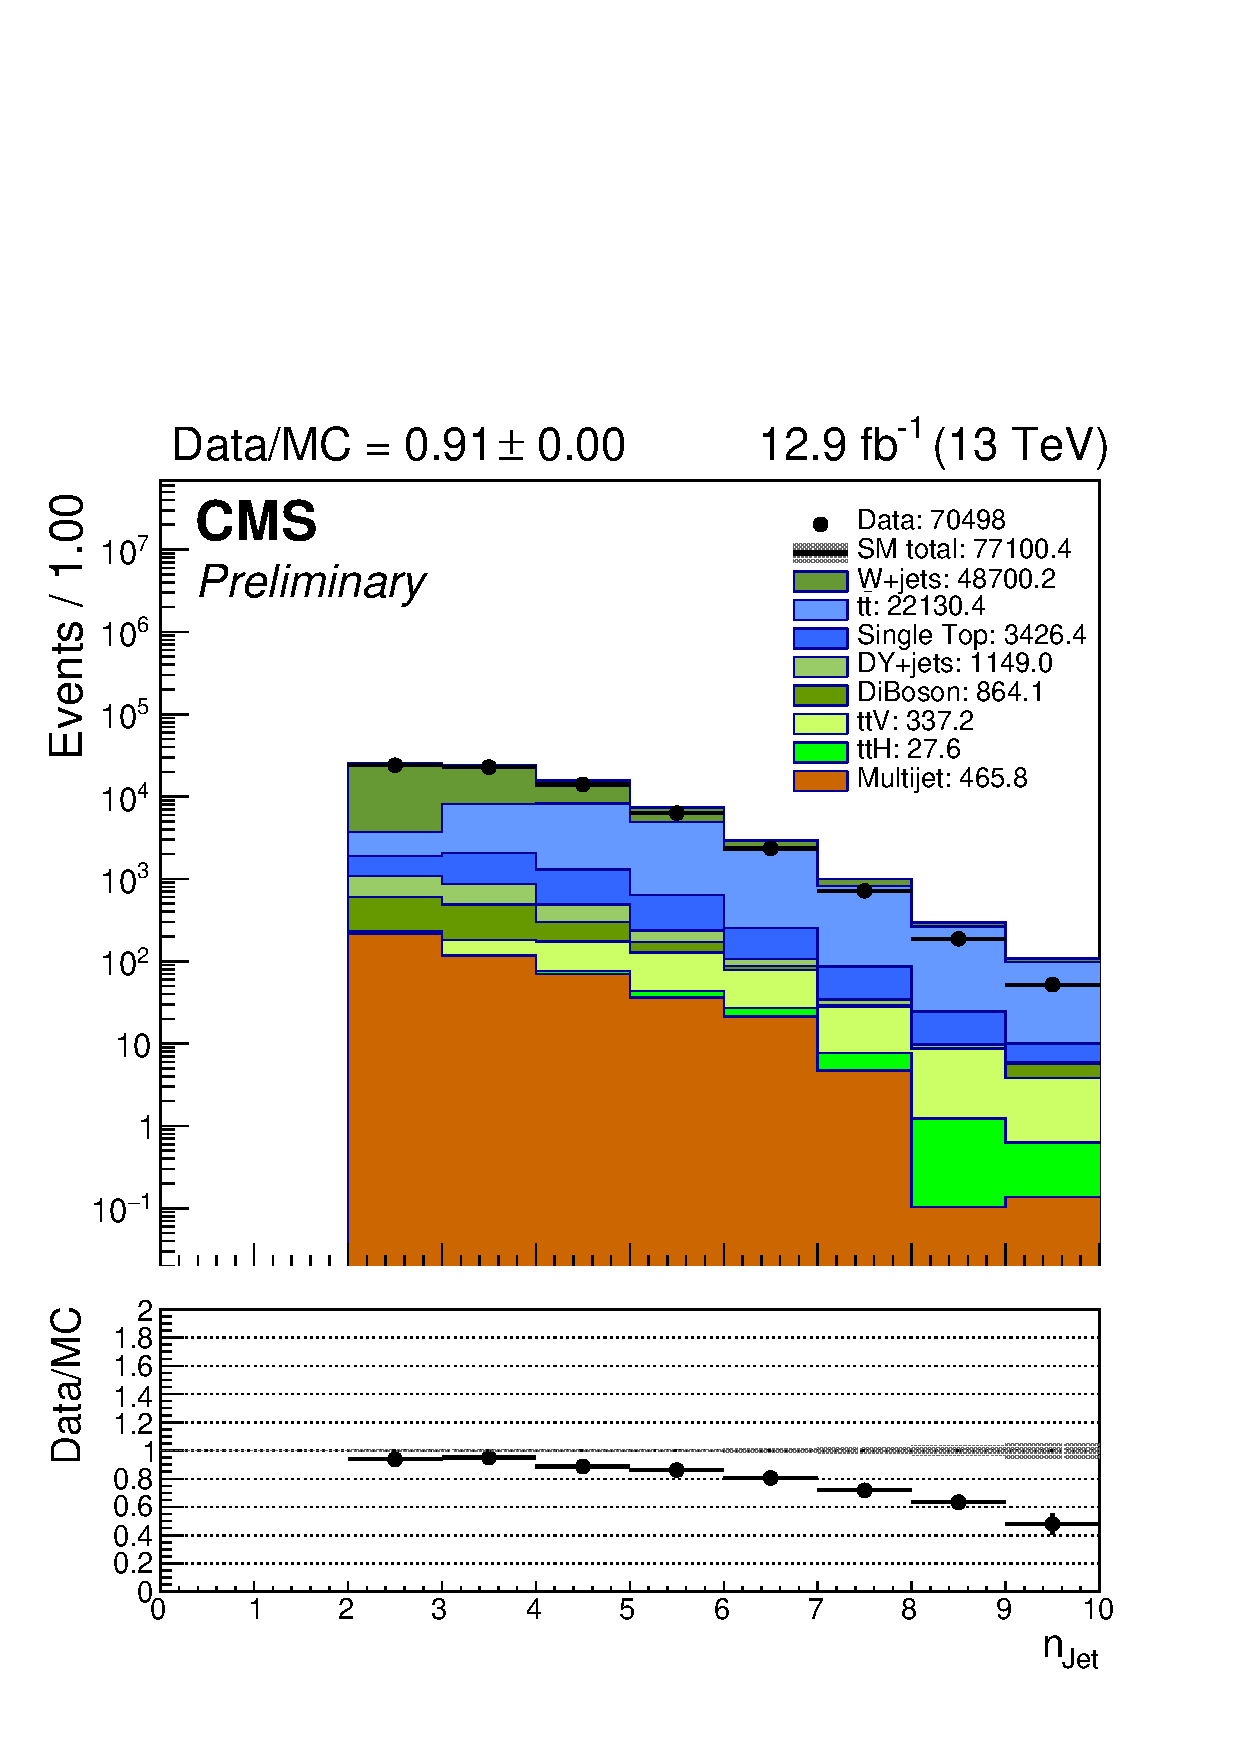
\includegraphics[width=0.5\textwidth]{figs/analysis/distributions/SingleMu/nJet40_sym.pdf}} ~~
        \subfloat {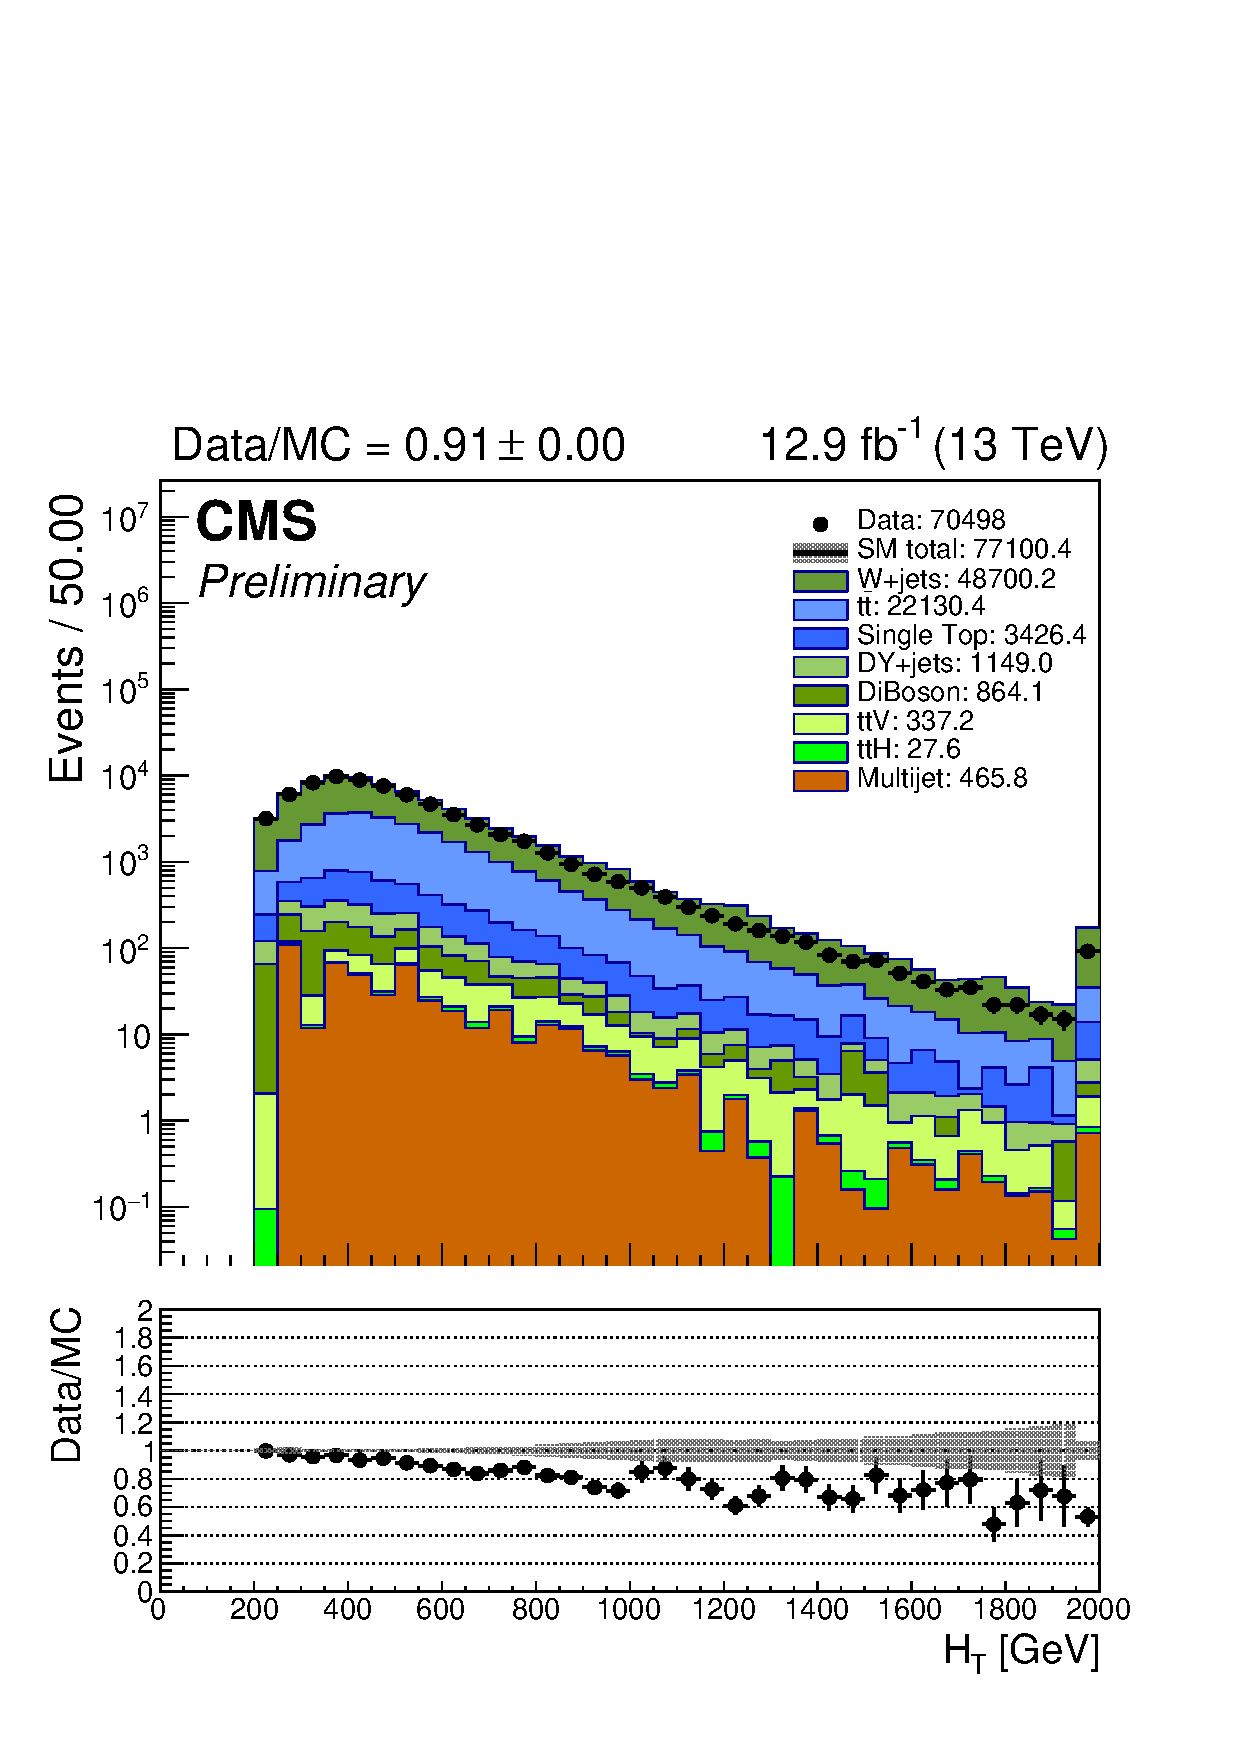
\includegraphics[width=0.5\textwidth]{figs/analysis/distributions/SingleMu/ht40_sym.pdf}} \\
        \subfloat {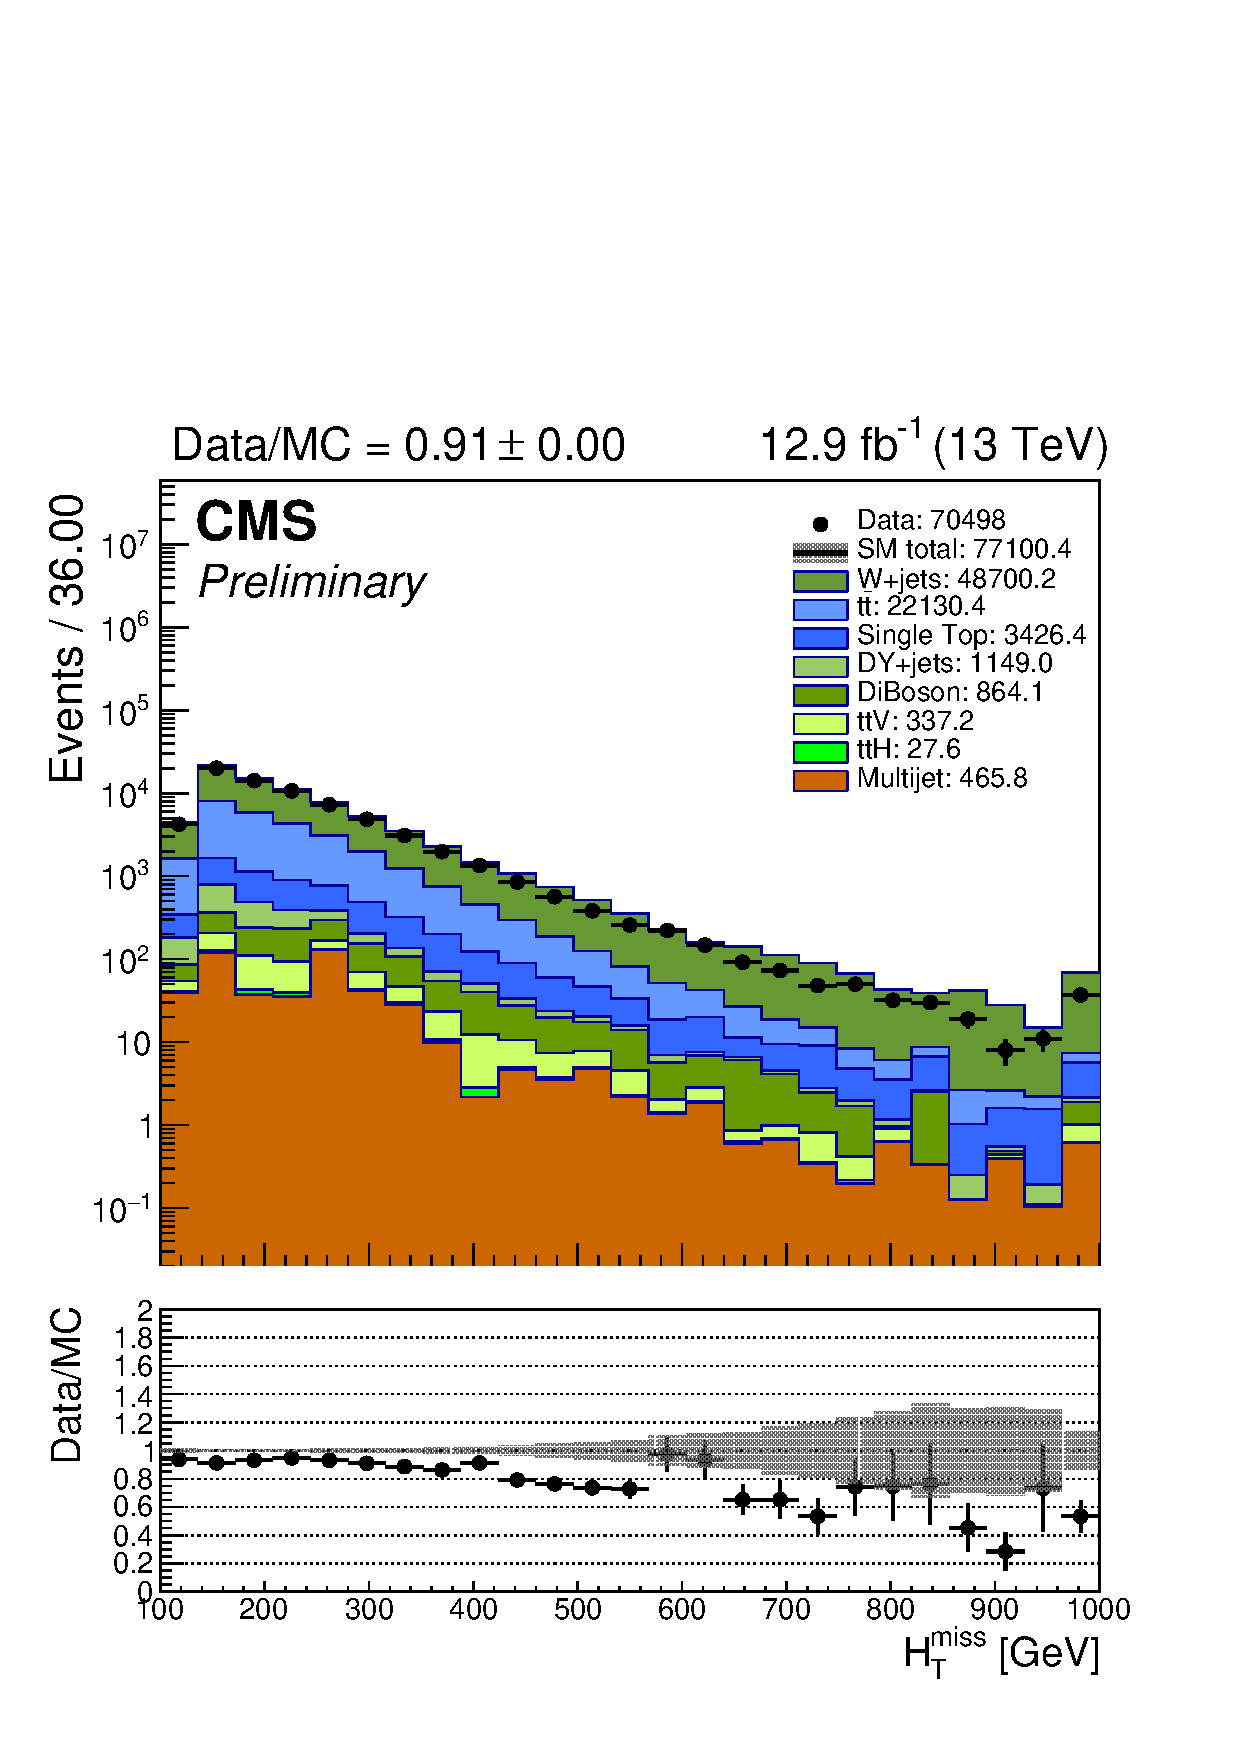
\includegraphics[width=0.5\textwidth]{figs/analysis/distributions/SingleMu/mht40_pt_sym.pdf}} ~~
        \subfloat {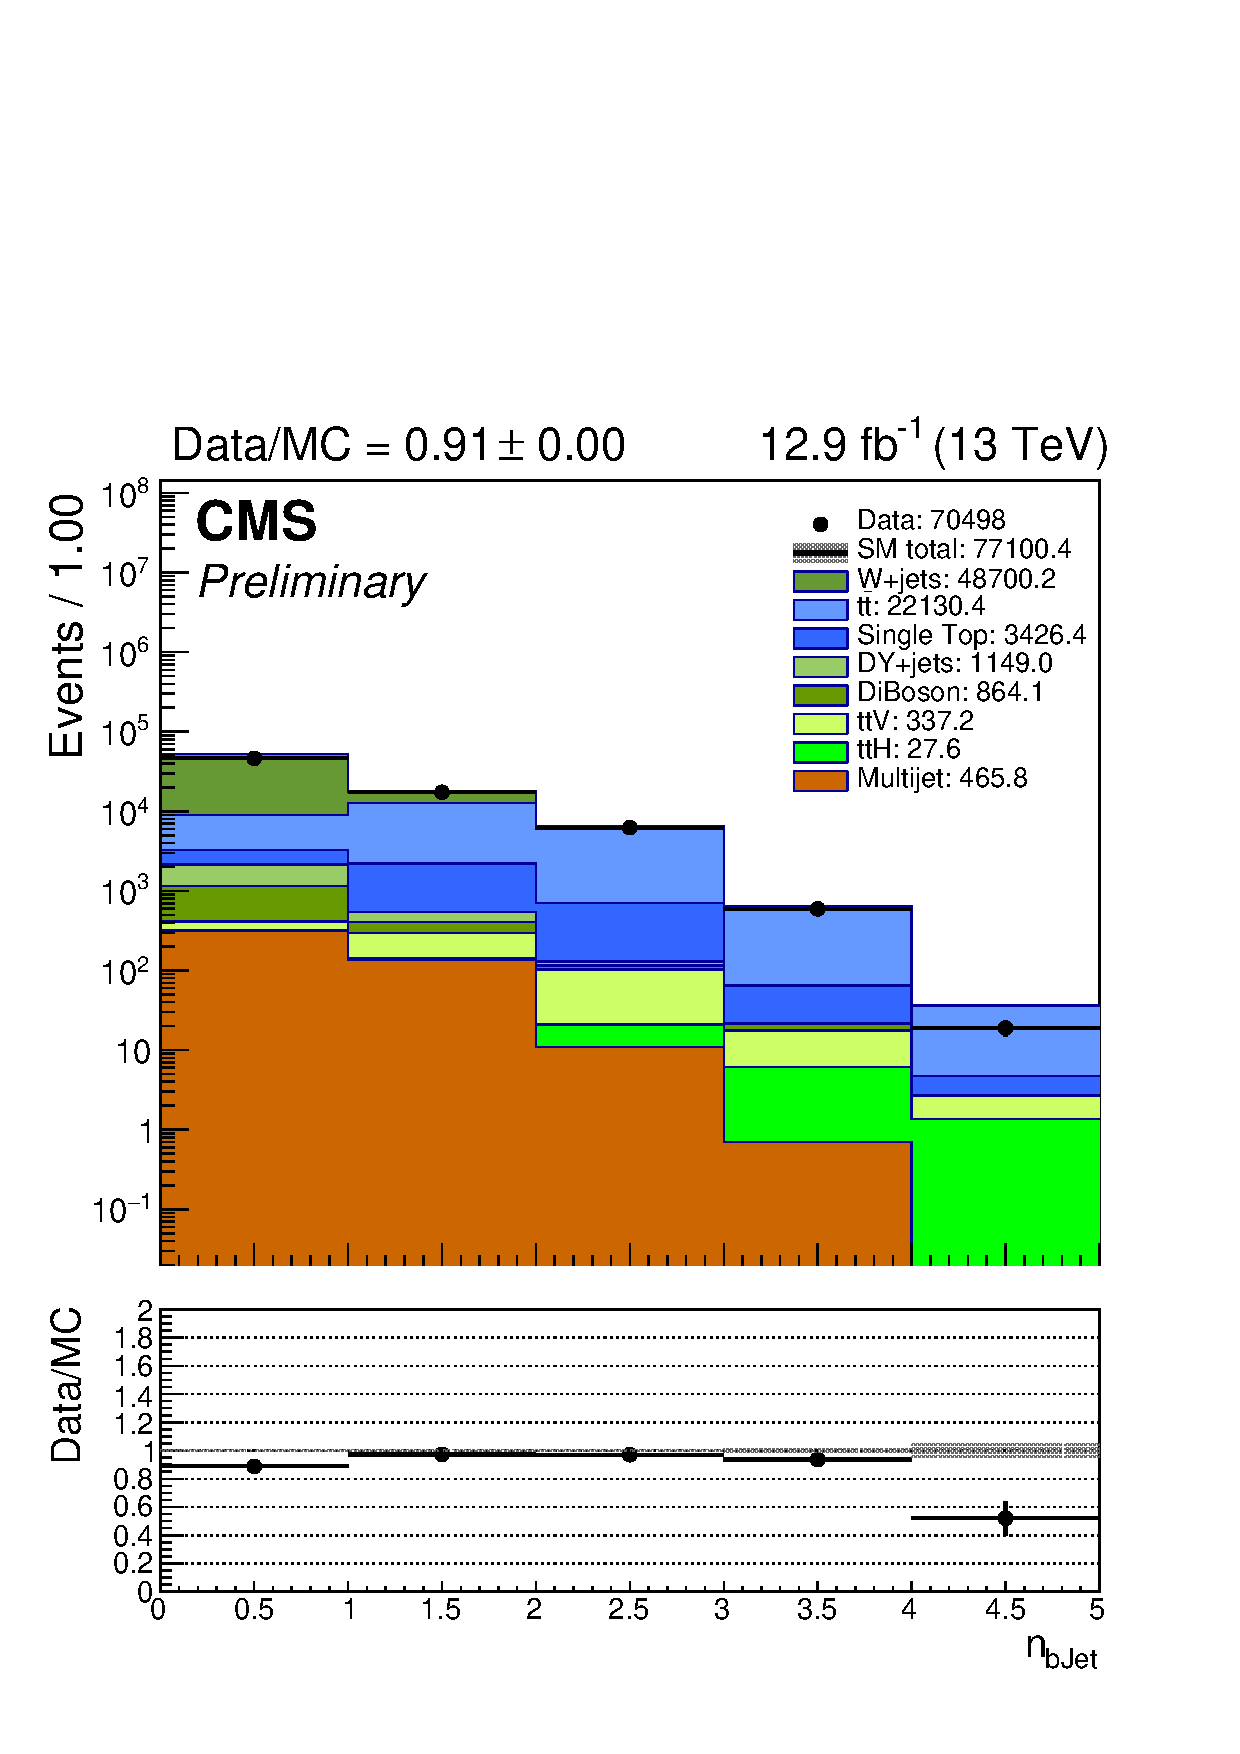
\includegraphics[width=0.5\textwidth]{figs/analysis/distributions/SingleMu/nBJet40_sym.pdf}} \\
        \caption{Key analysis variables for single muon control region (symmetric \njet bins)}
        \label{fig:distribution_singlemu_sym}
    \end{center}
\end{figure}

\clearpage
\begin{figure}
    \begin{center}
        \subfloat {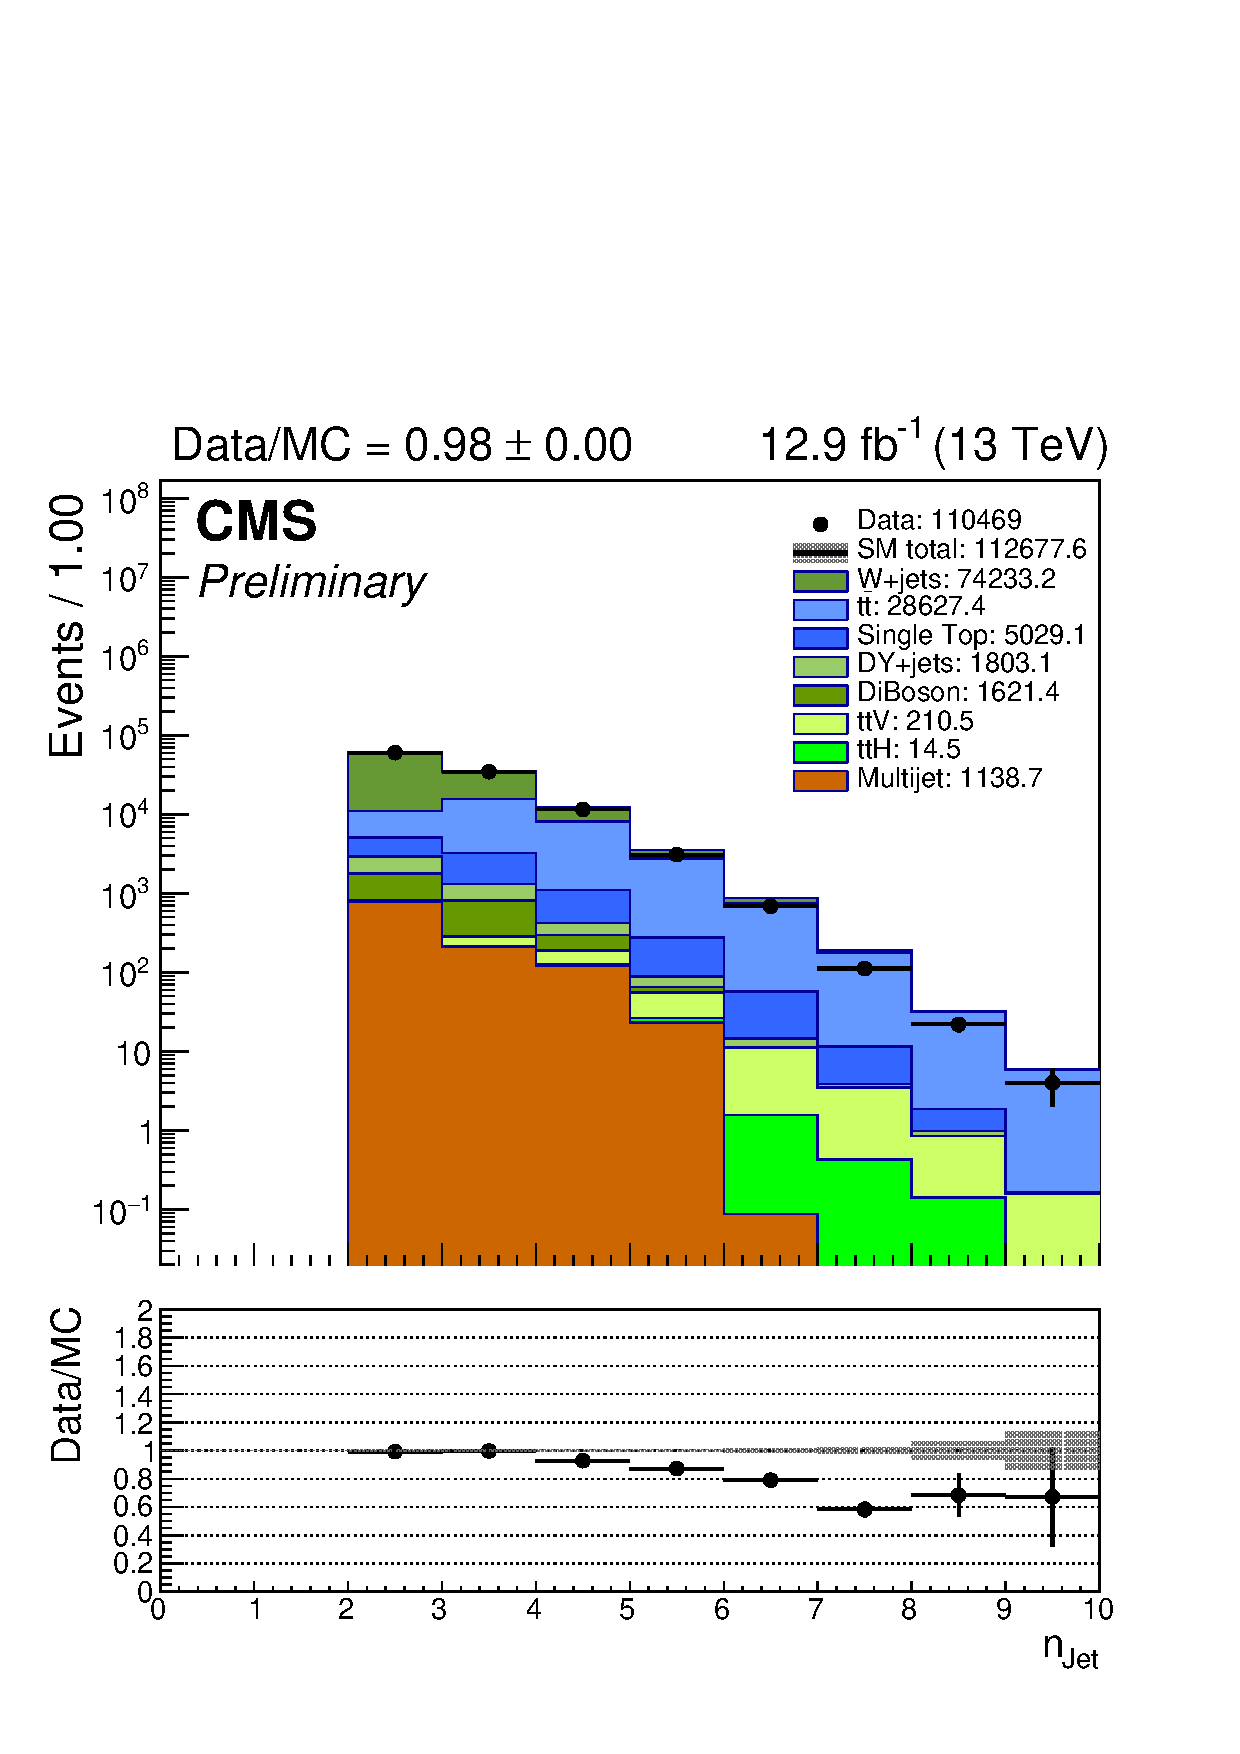
\includegraphics[width=0.5\textwidth]{figs/analysis/distributions/SingleMu/nJet40_asym.pdf}} ~~
        \subfloat {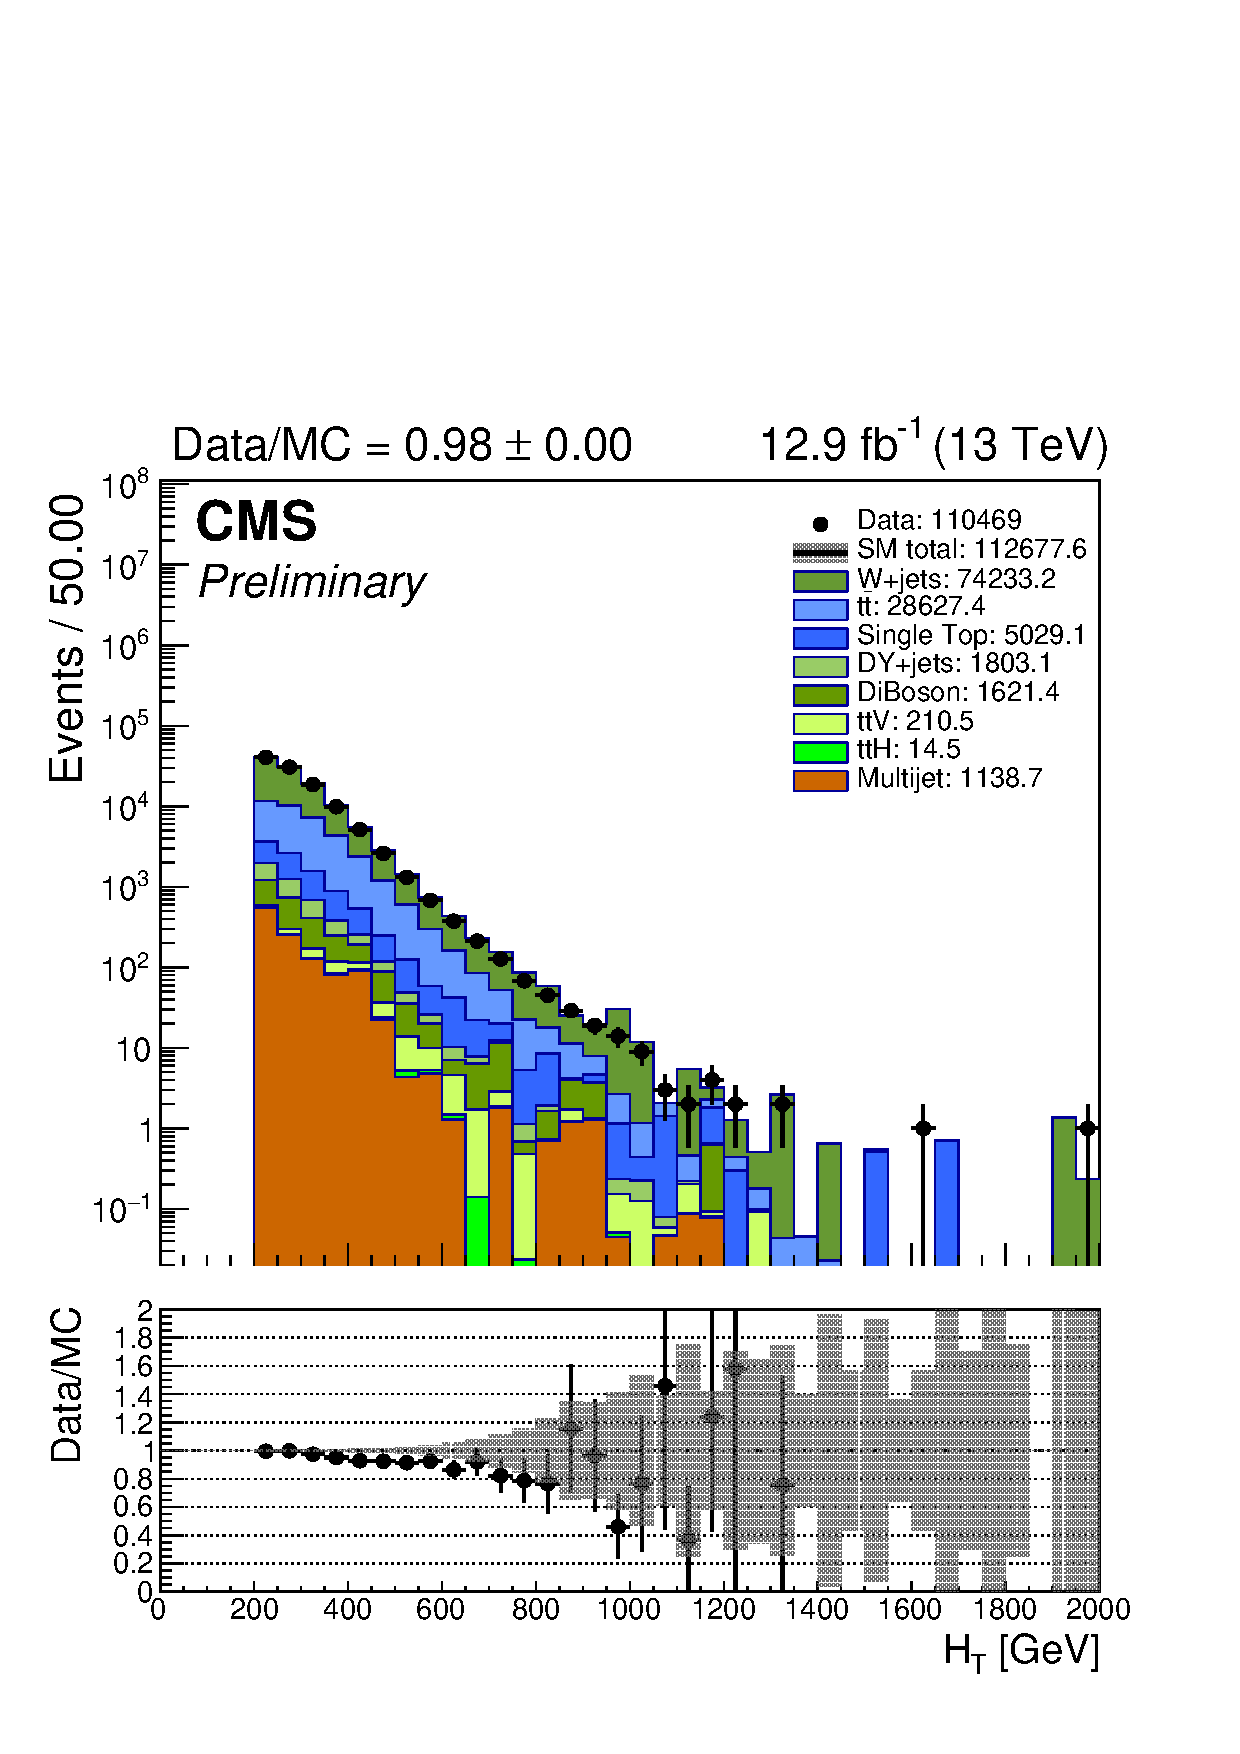
\includegraphics[width=0.5\textwidth]{figs/analysis/distributions/SingleMu/ht40_asym.pdf}} \\
        \subfloat {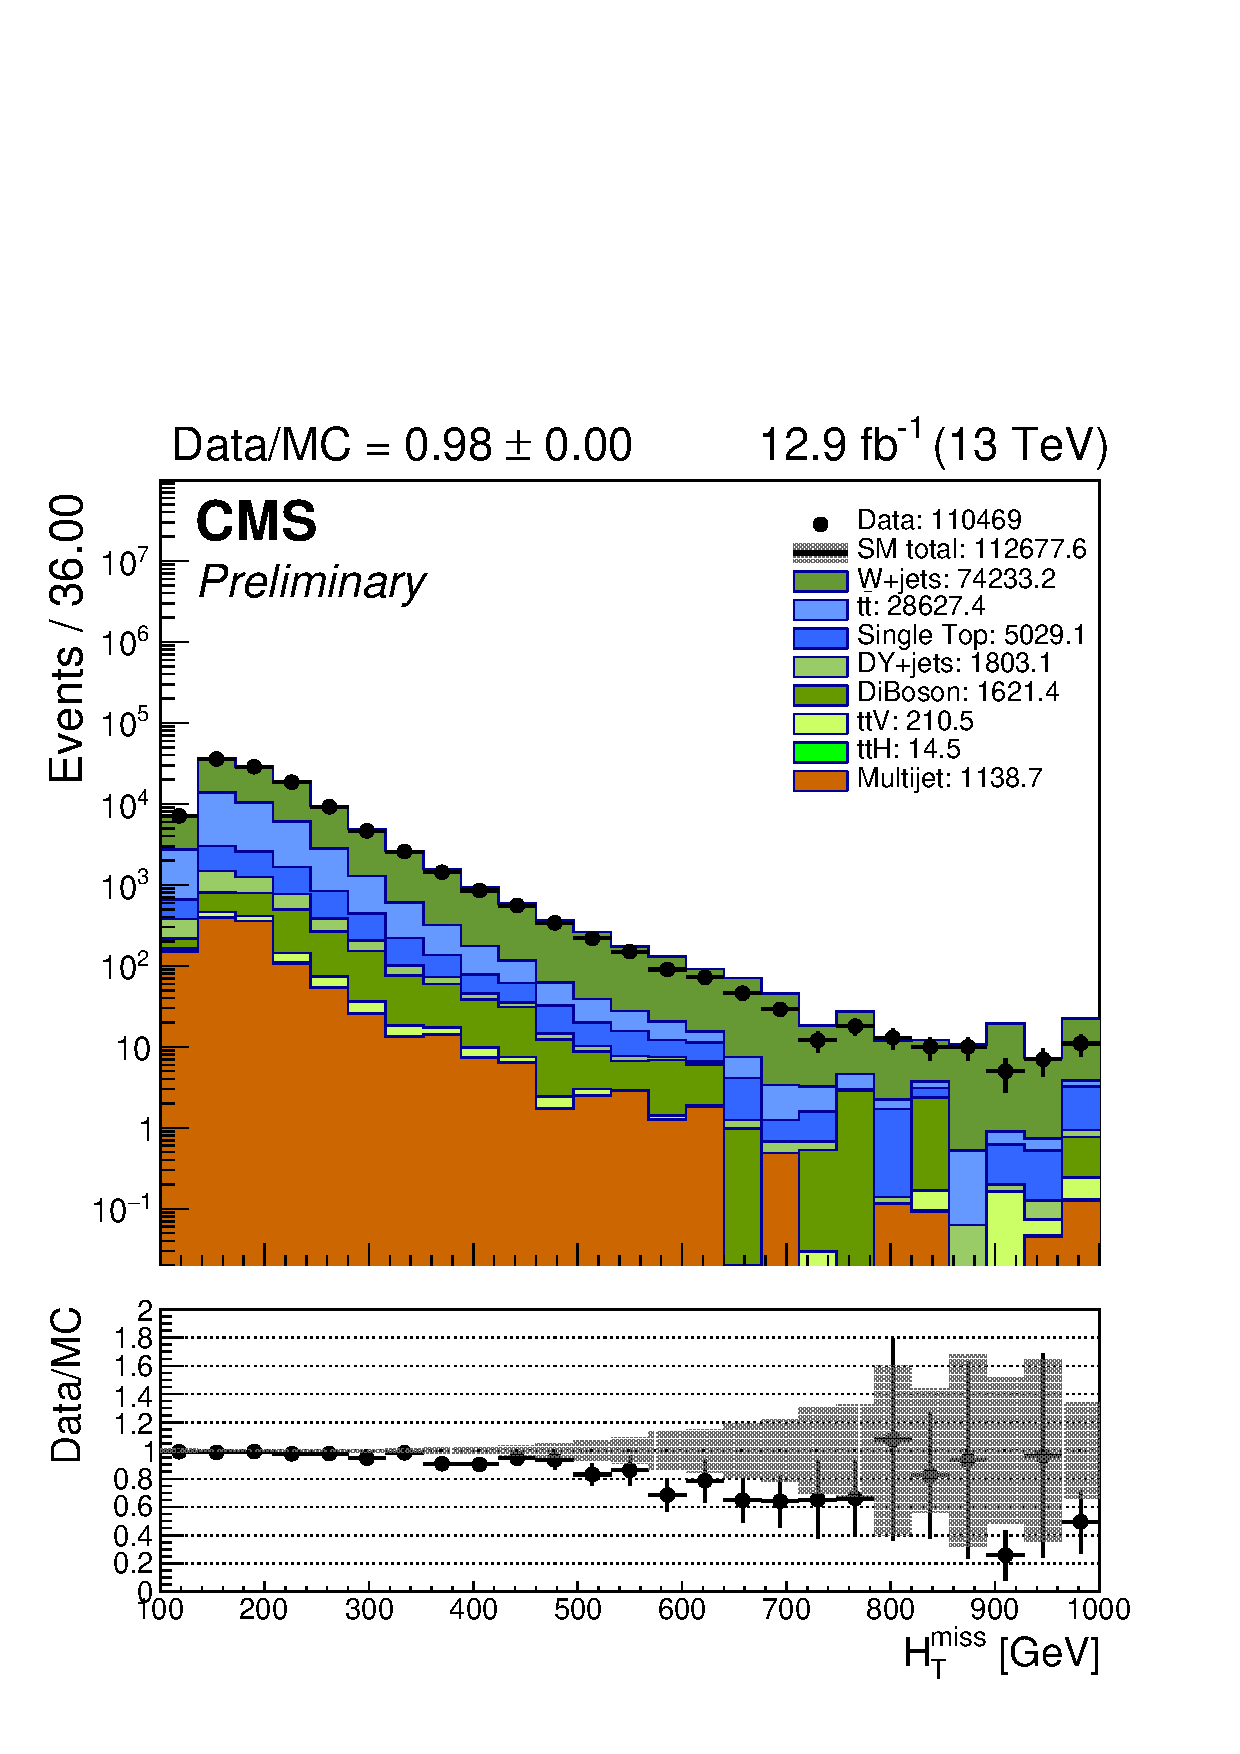
\includegraphics[width=0.5\textwidth]{figs/analysis/distributions/SingleMu/mht40_pt_asym.pdf}} ~~
        \subfloat {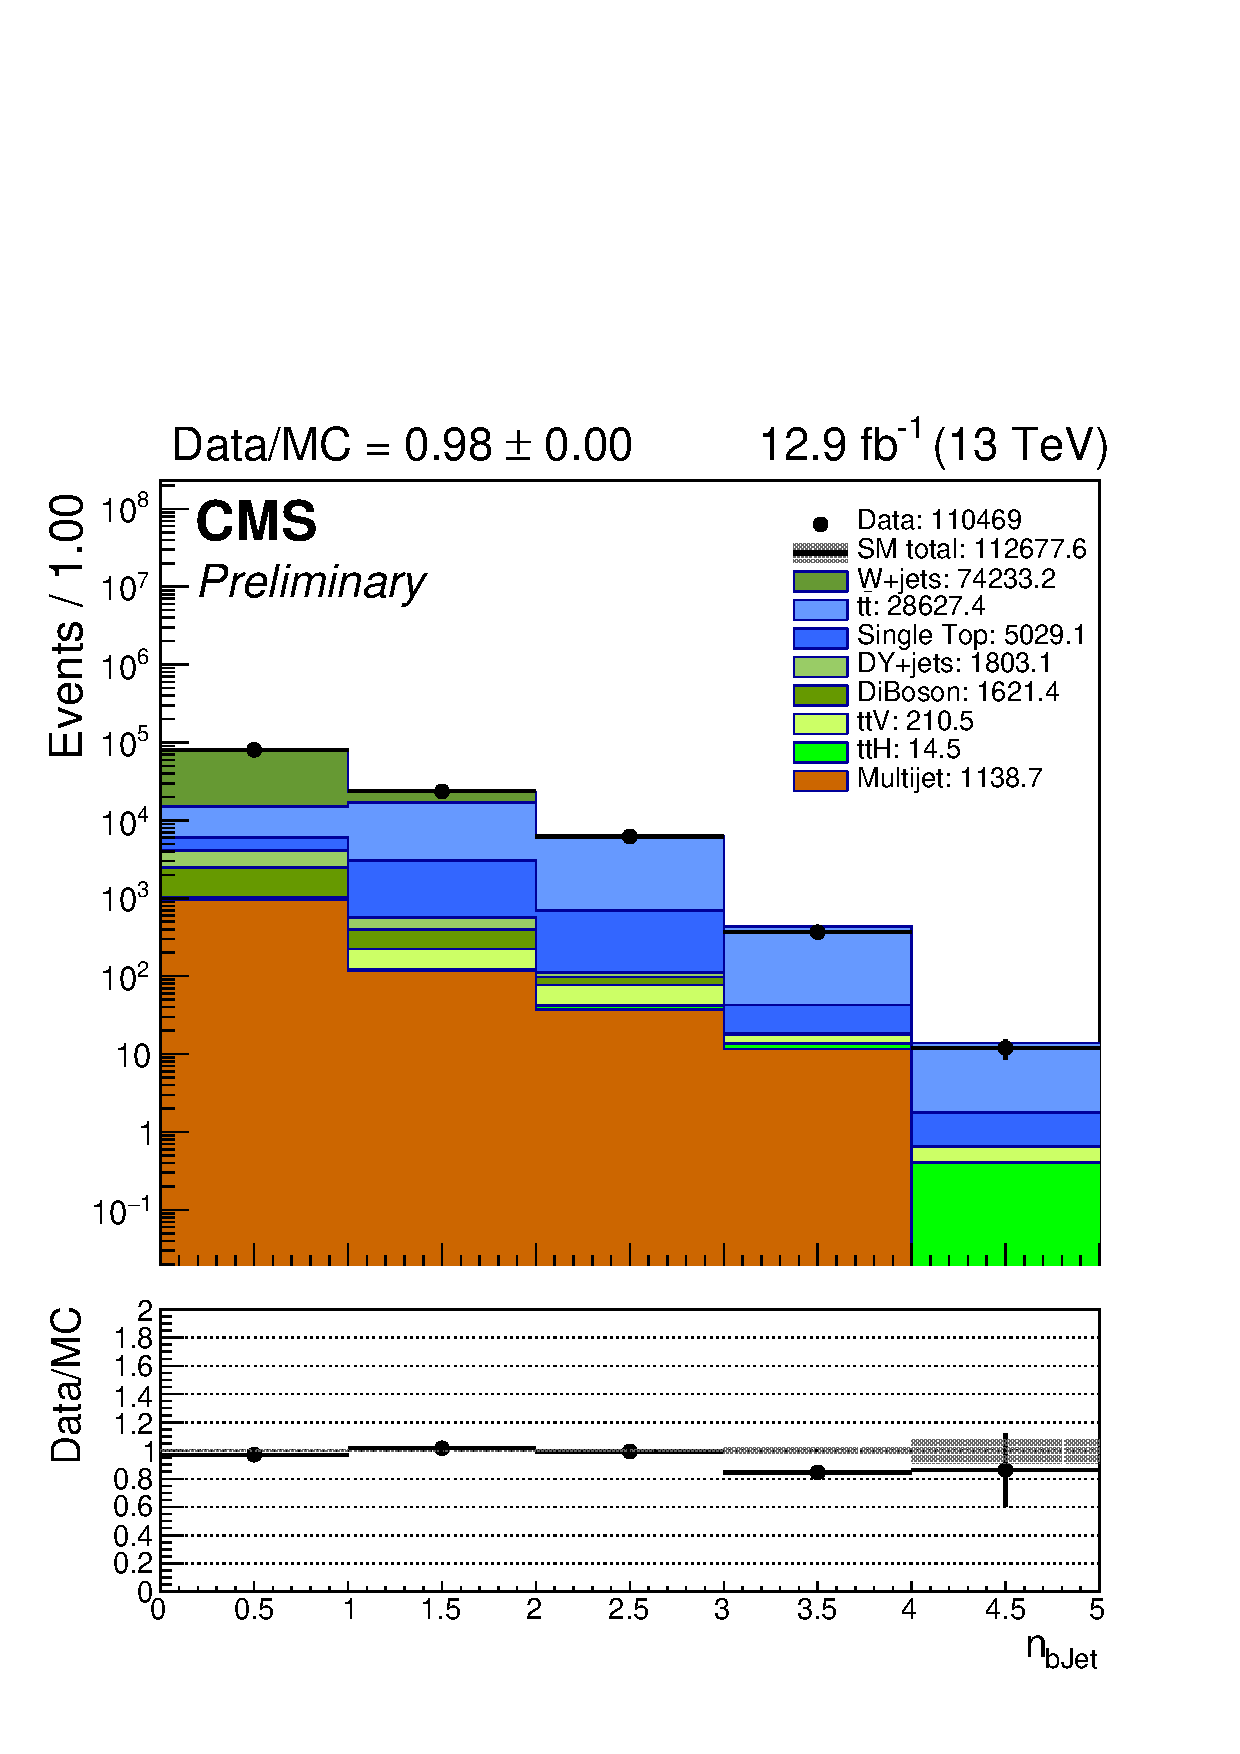
\includegraphics[width=0.5\textwidth]{figs/analysis/distributions/SingleMu/nBJet40_asym.pdf}} \\
        \caption{Key analysis variables for single muon control region (asymmetric \njet bins)}
        \label{fig:distribution_singlemu_asym}
    \end{center}
\end{figure}

\clearpage
\begin{figure}
    \begin{center}        
        \subfloat {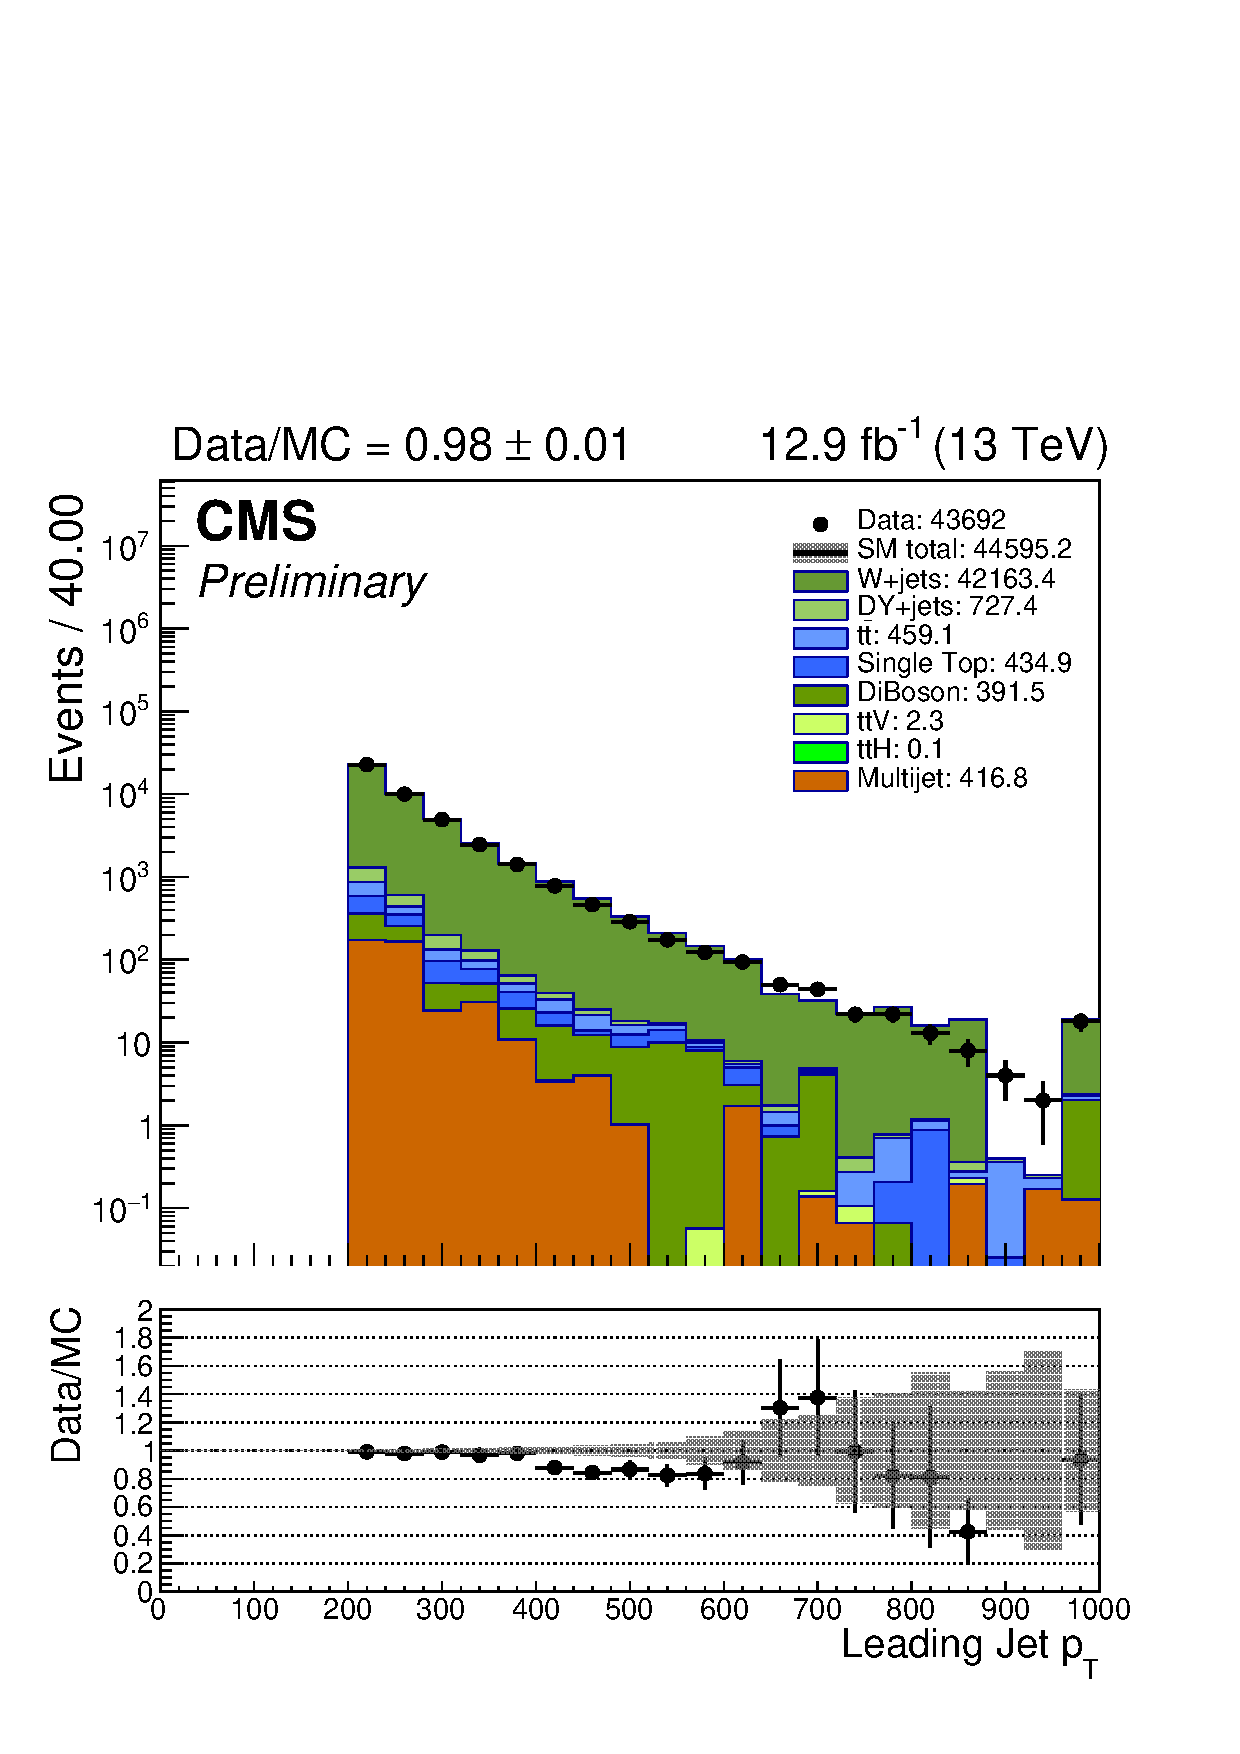
\includegraphics[width=0.5\textwidth]{figs/analysis/distributions/SingleMu/jet_pt[0]_eq1j.pdf}} ~~
        \subfloat {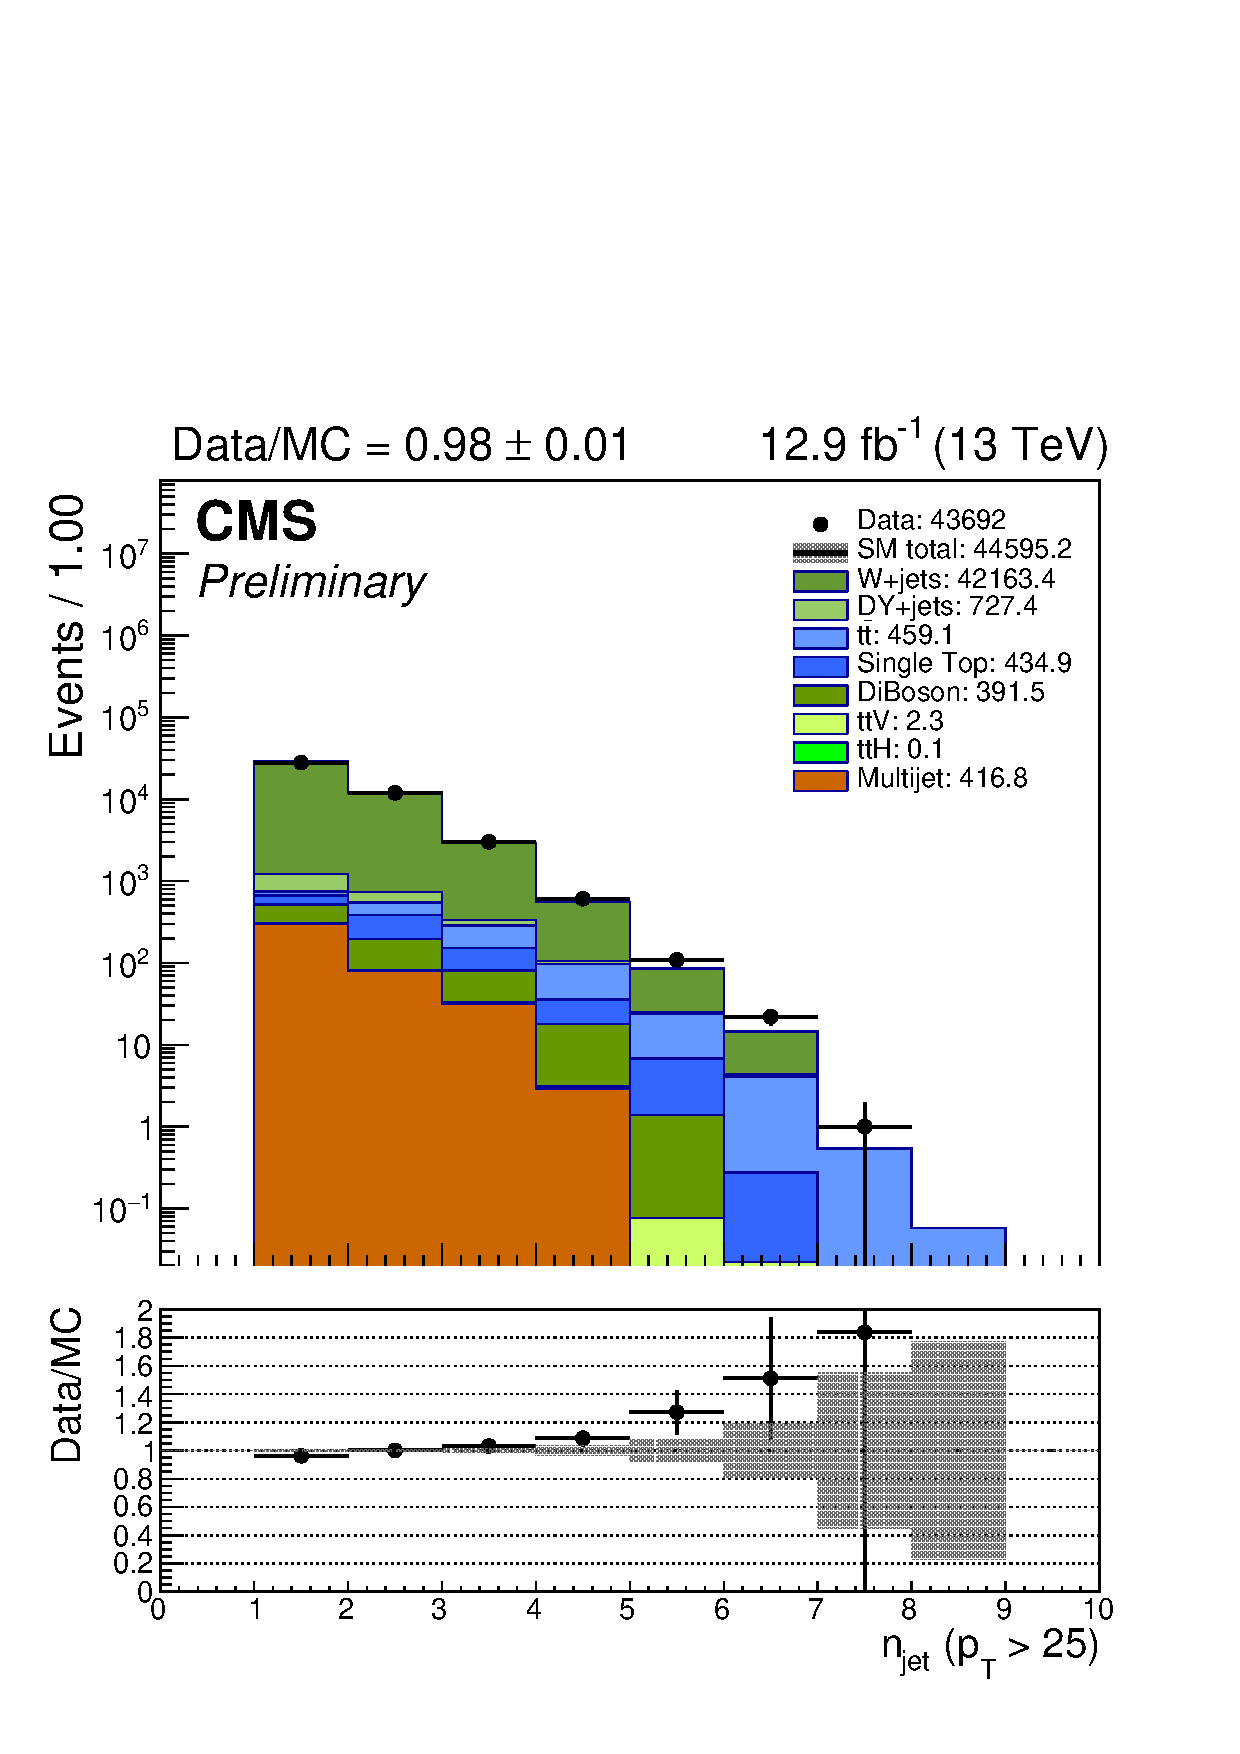
\includegraphics[width=0.5\textwidth]{figs/analysis/distributions/SingleMu/njetInc_eq1j.pdf}} \\
        \subfloat {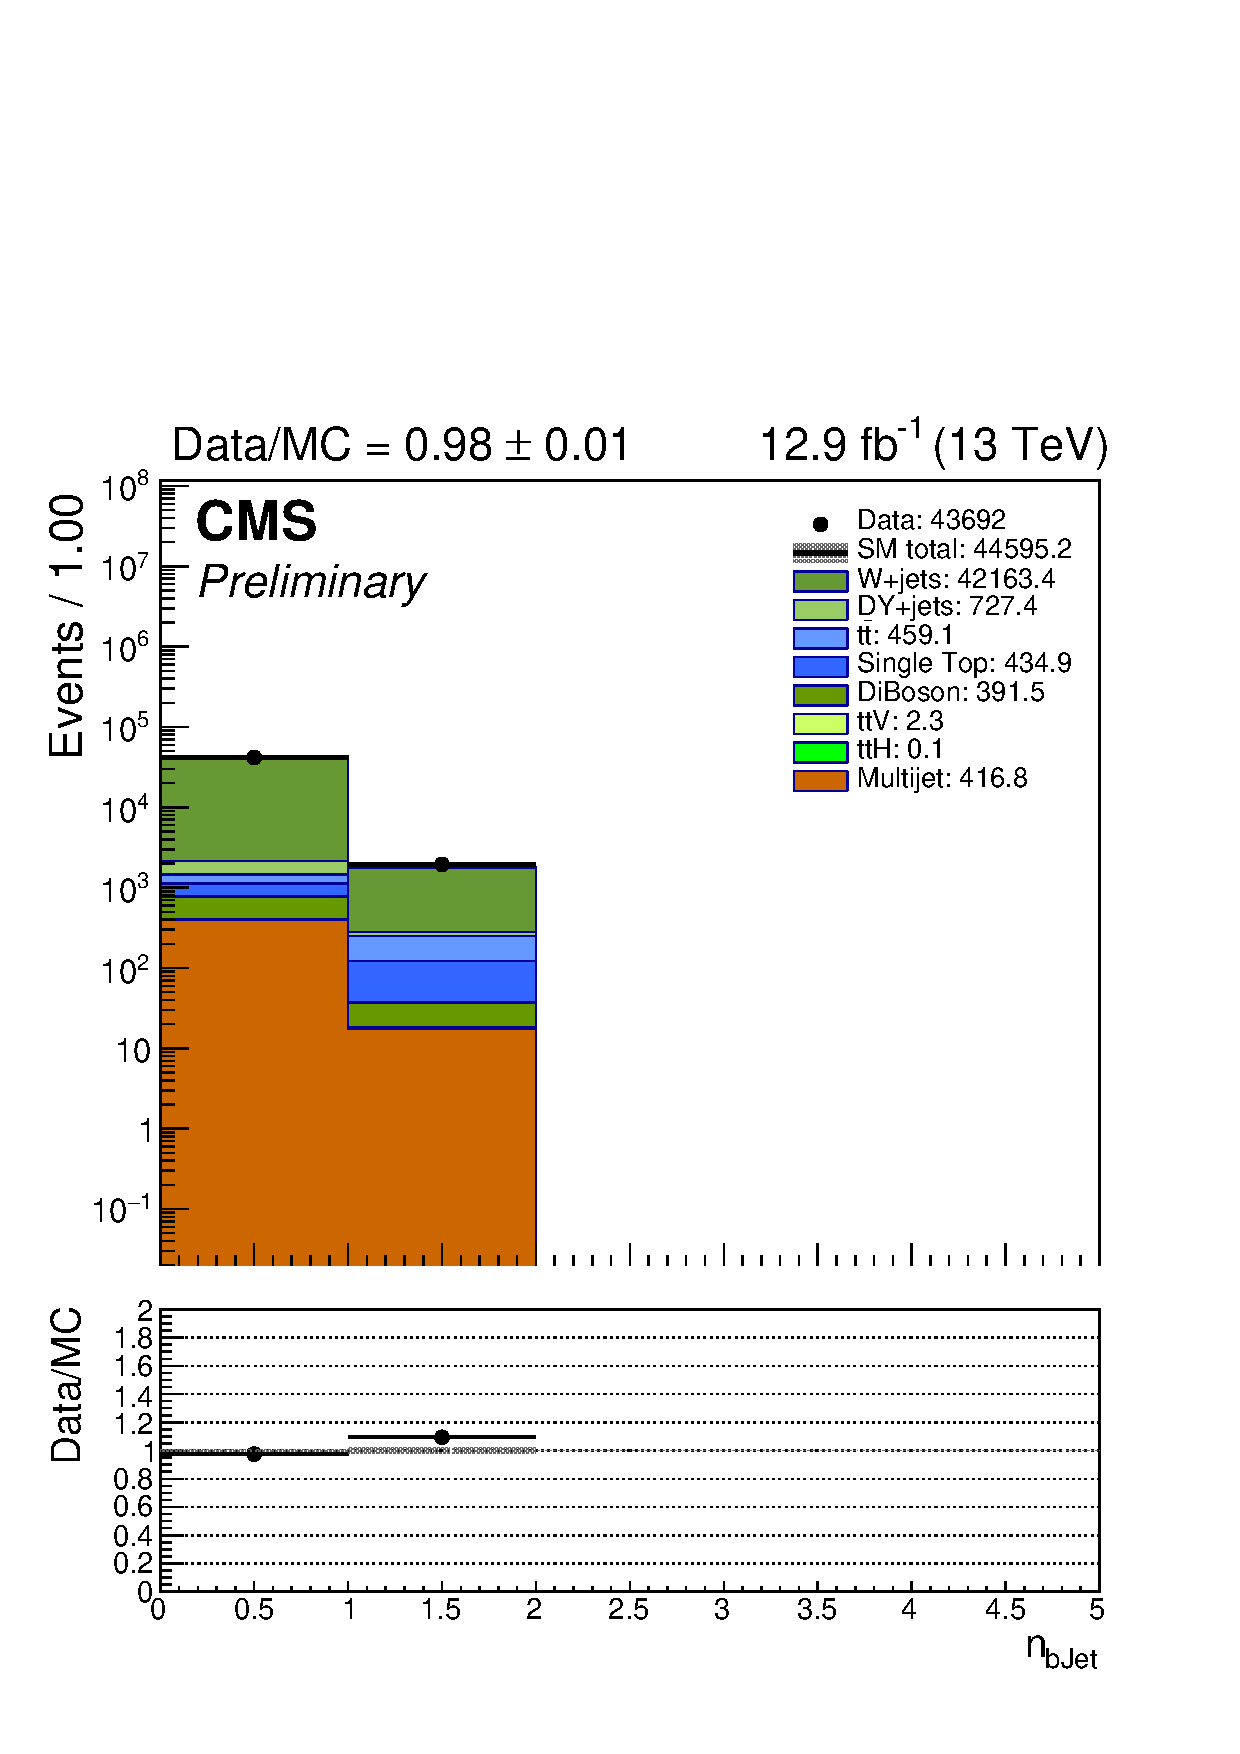
\includegraphics[width=0.5\textwidth]{figs/analysis/distributions/SingleMu/nBJet40_eq1j.pdf}} ~~
        \subfloat {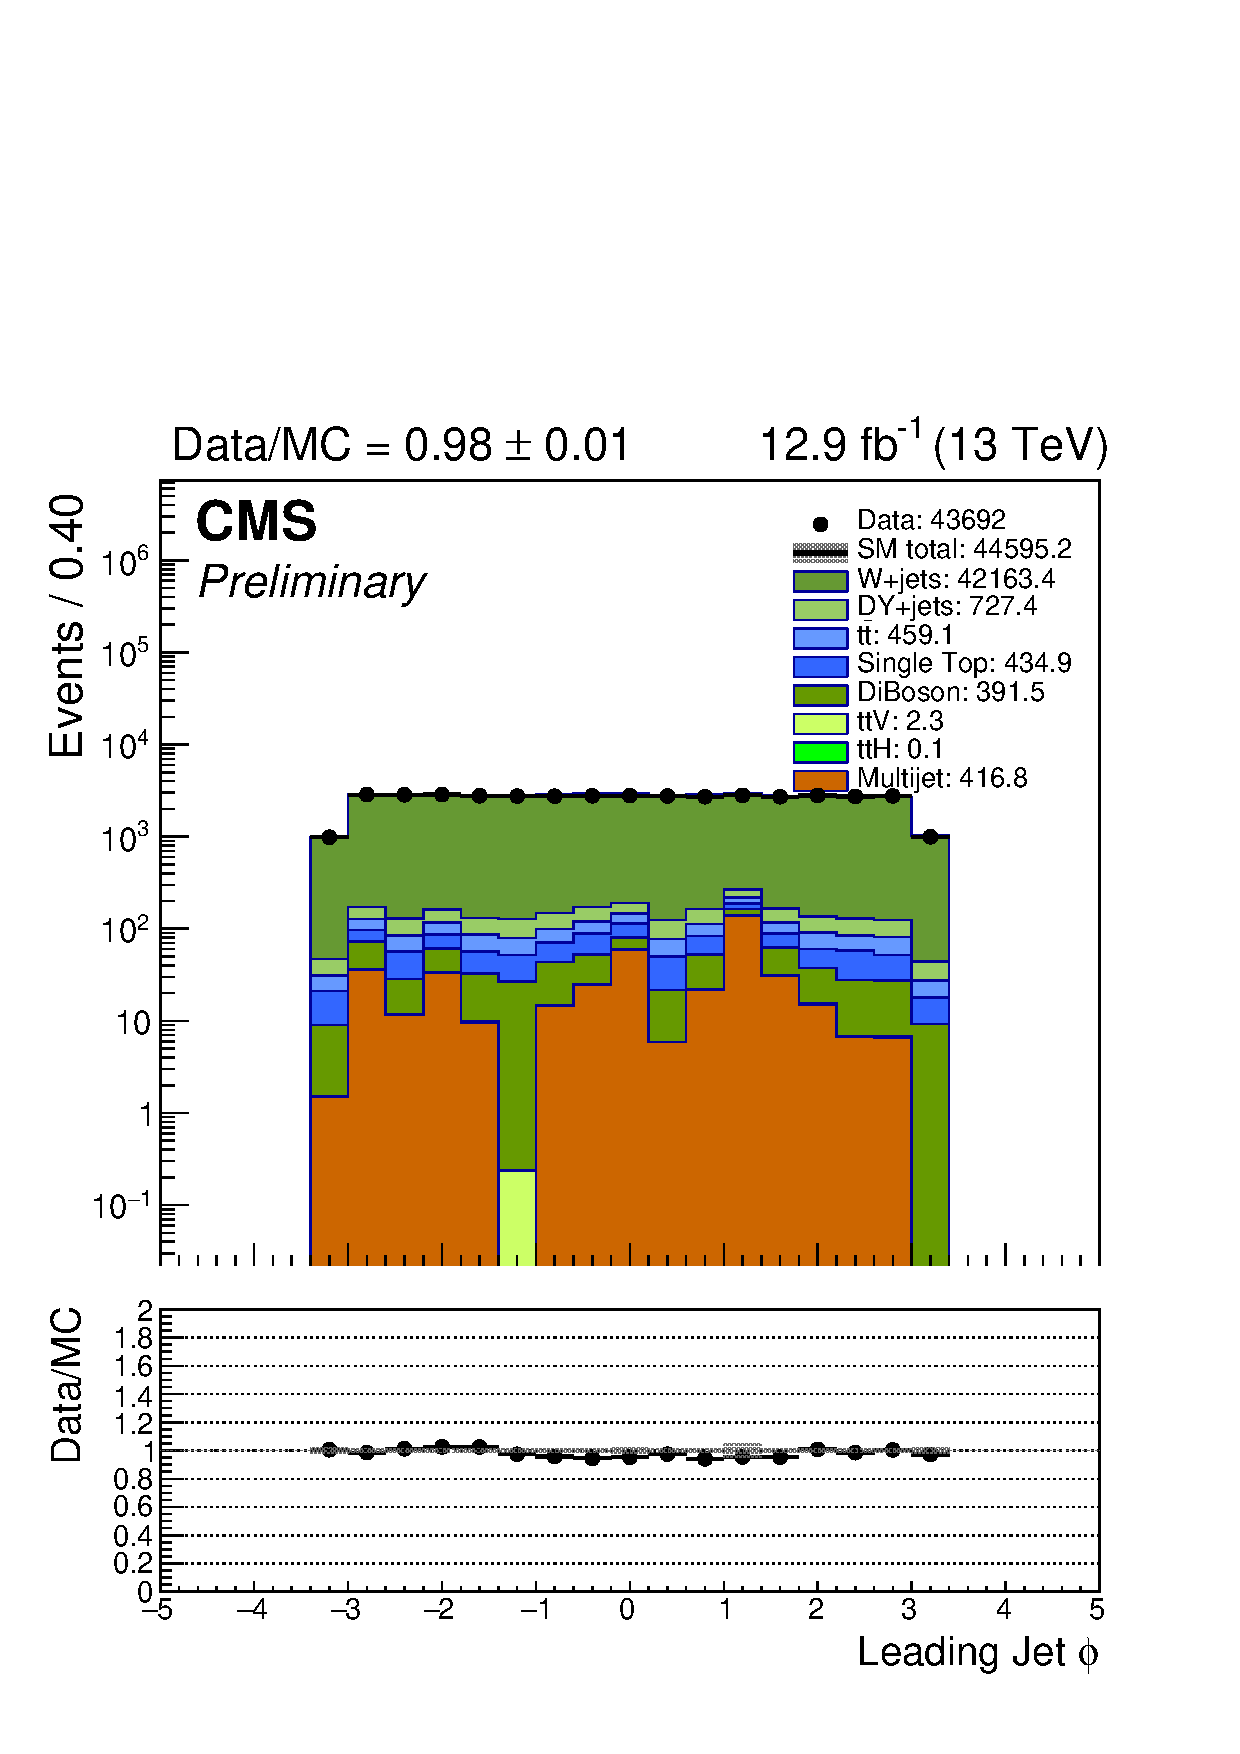
\includegraphics[width=0.5\textwidth]{figs/analysis/distributions/SingleMu/jet_phi[0]_eq1j.pdf}} \\
        \caption{Key analysis variables for single muon control region (monojet bins)}
        \label{fig:distribution_singlemu_mono}
    \end{center}
\end{figure}

% \clearpage
% \subsection{Yields and distributions for the di-muon + jets control sample}

\begin{figure}
    \begin{center}
        \subfloat {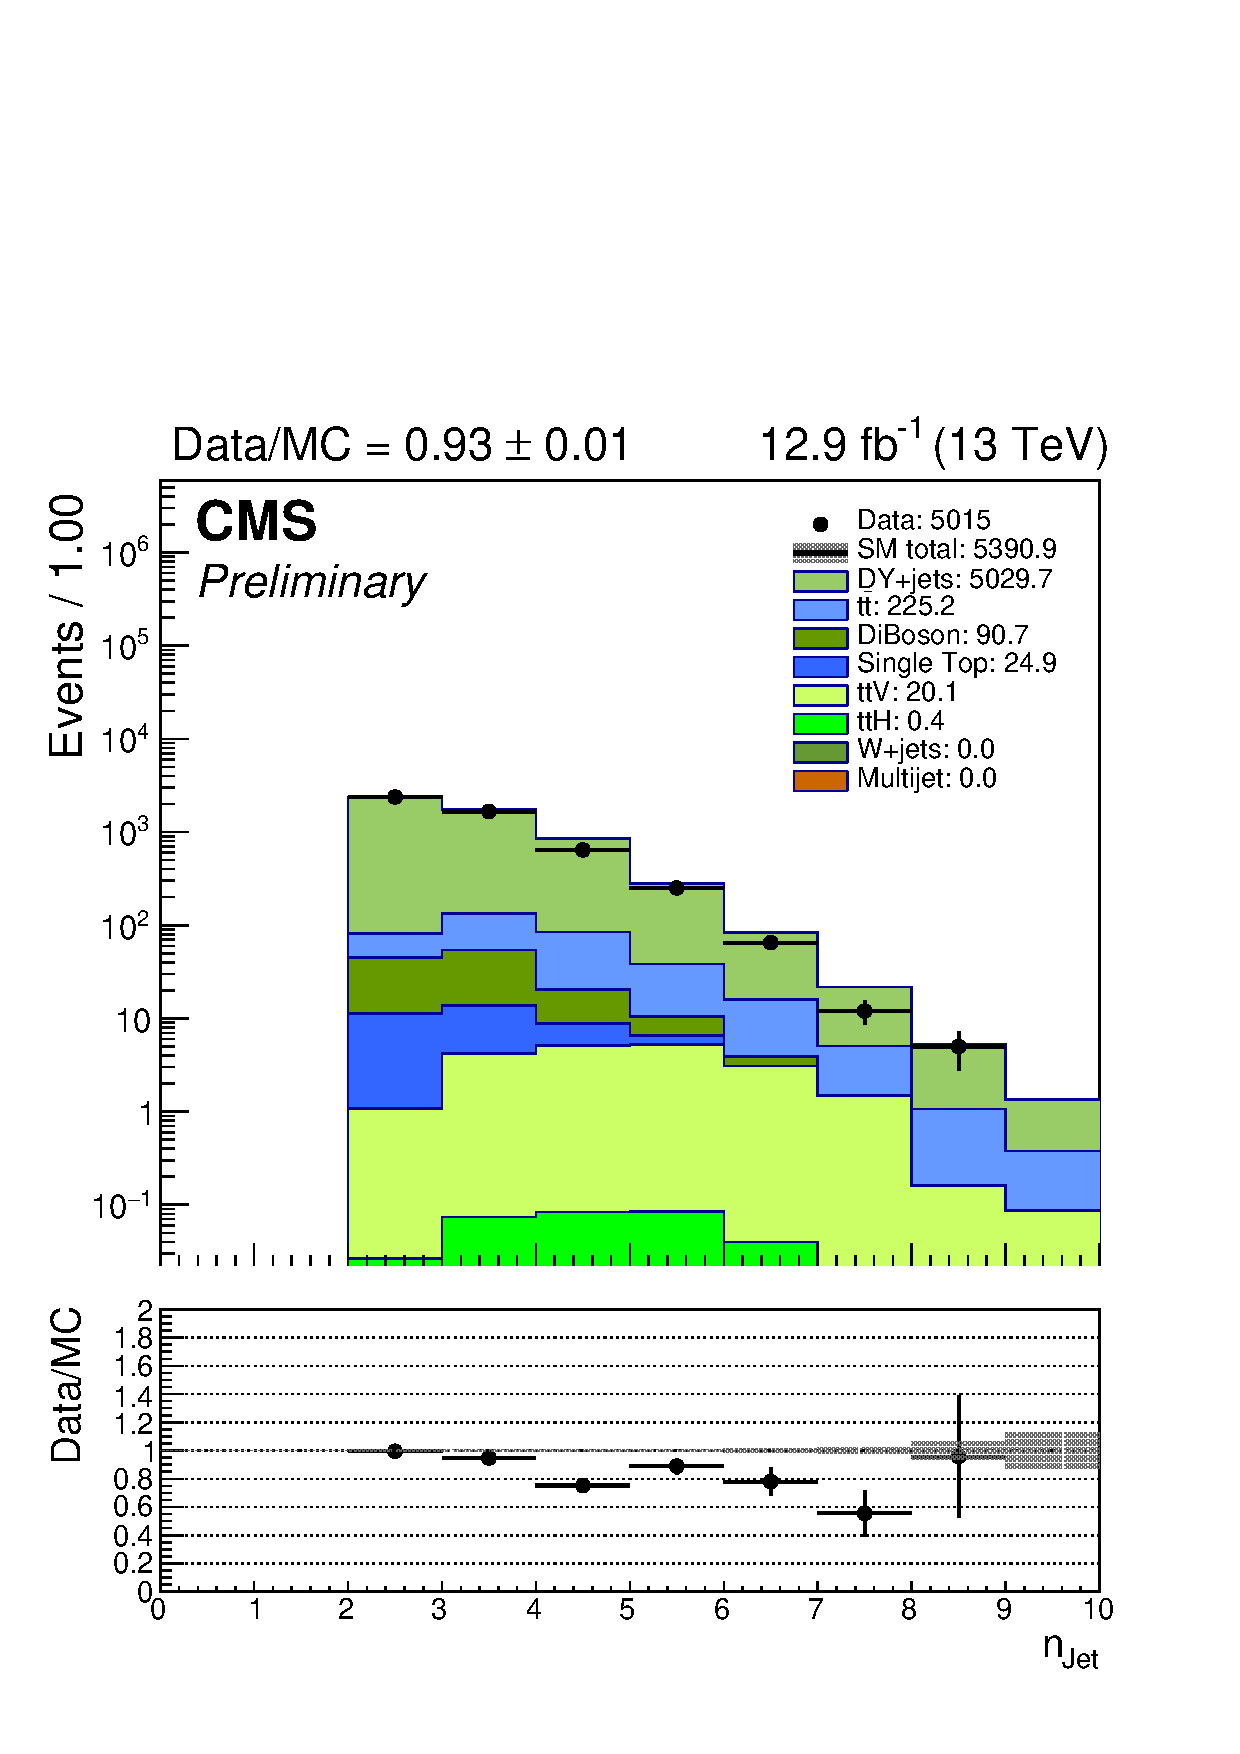
\includegraphics[width=0.5\textwidth]{figs/analysis/distributions/DoubleMu/nJet40_sym.pdf}} ~~
        \subfloat {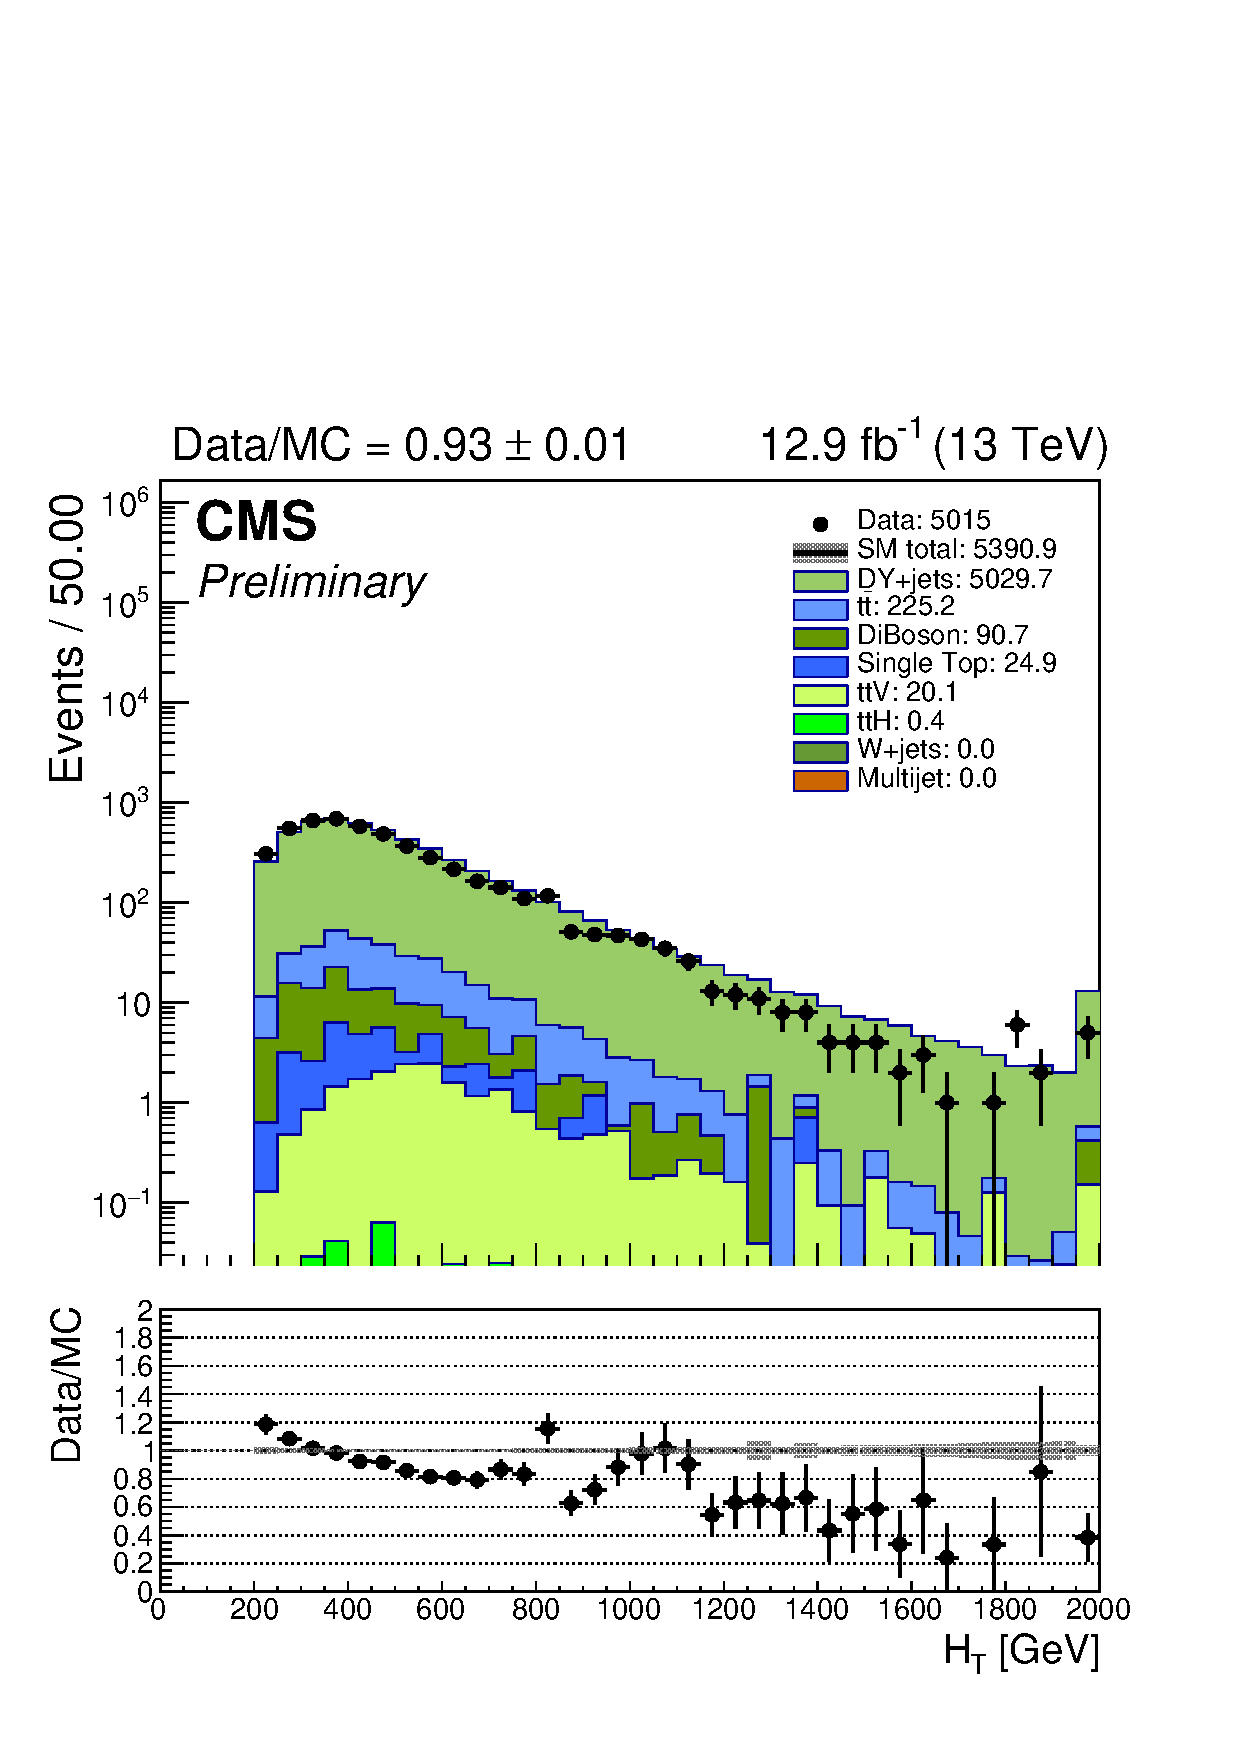
\includegraphics[width=0.5\textwidth]{figs/analysis/distributions/DoubleMu/ht40_sym.pdf}} \\
        \subfloat {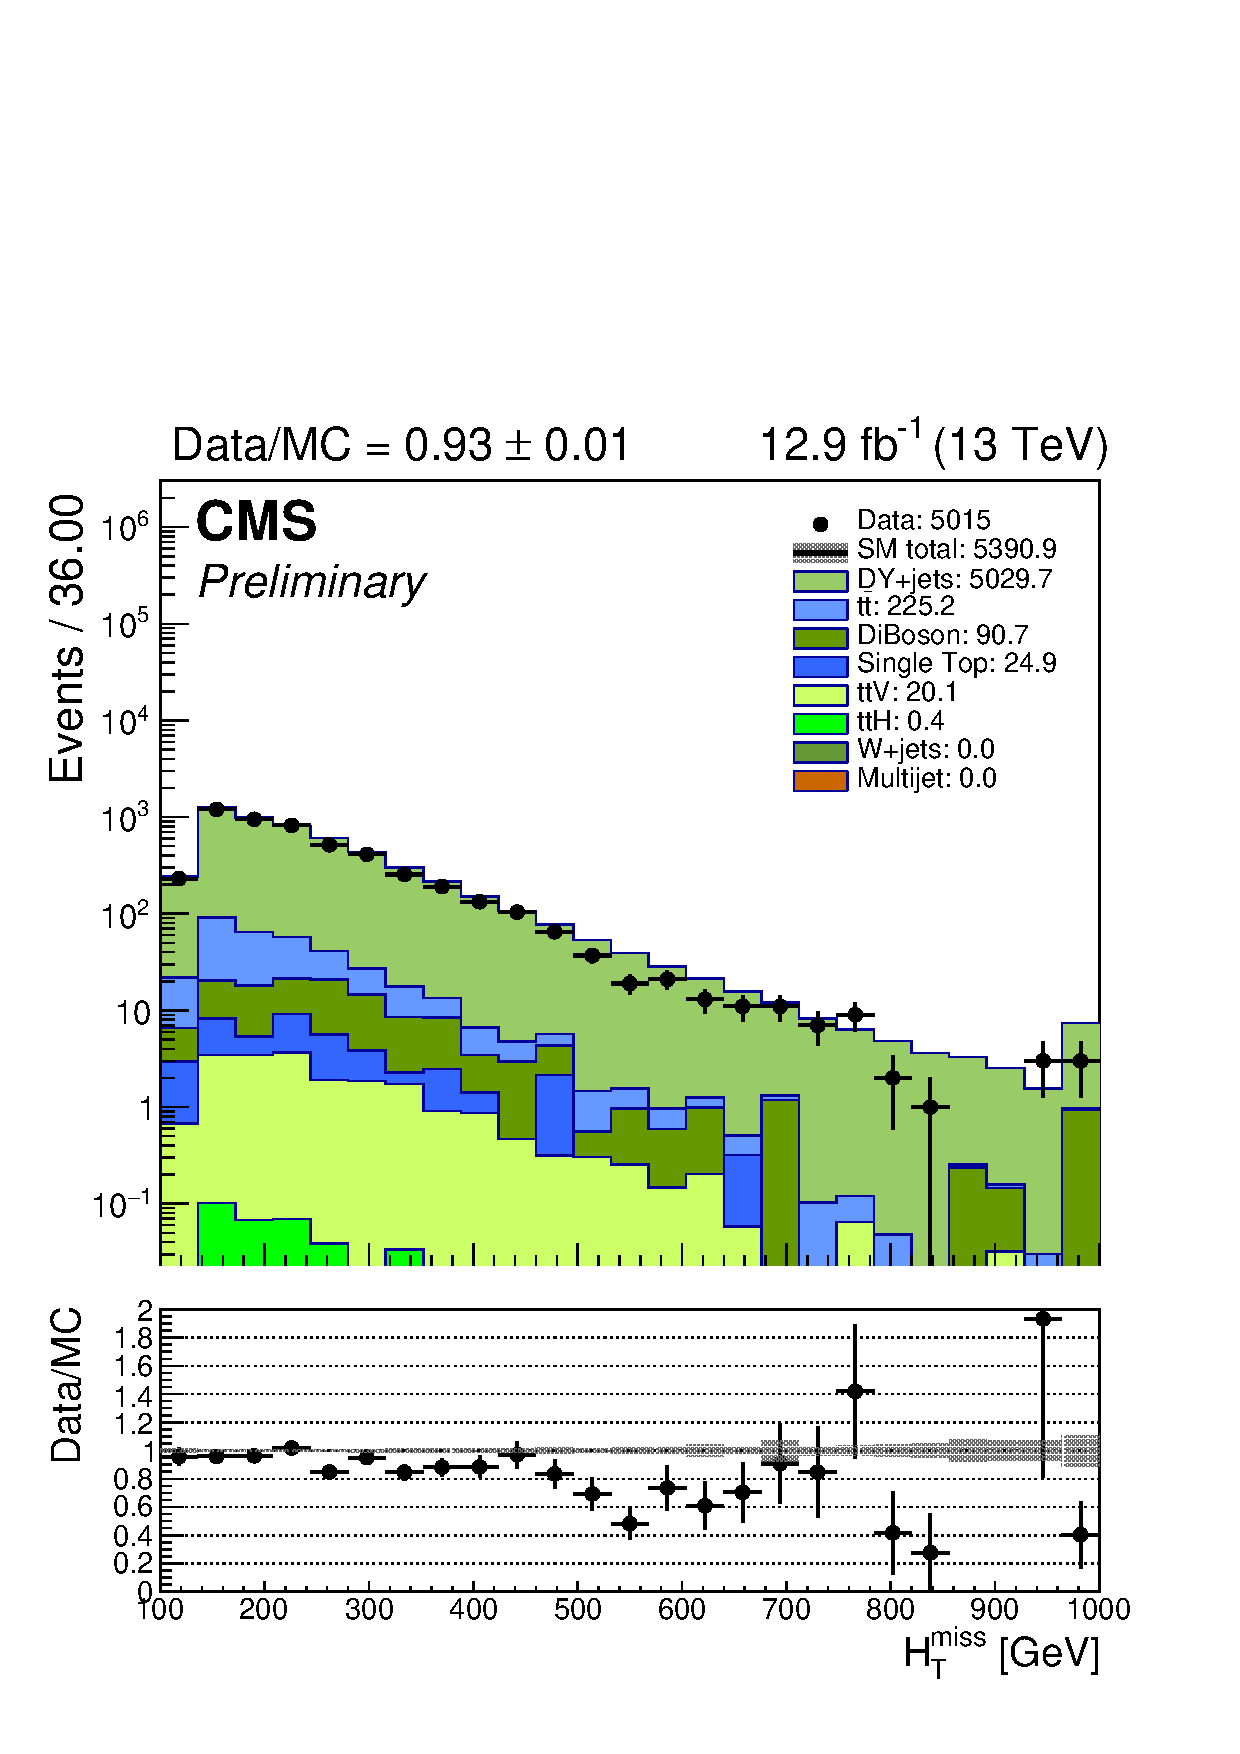
\includegraphics[width=0.5\textwidth]{figs/analysis/distributions/DoubleMu/mht40_pt_sym.pdf}} ~~
        \subfloat {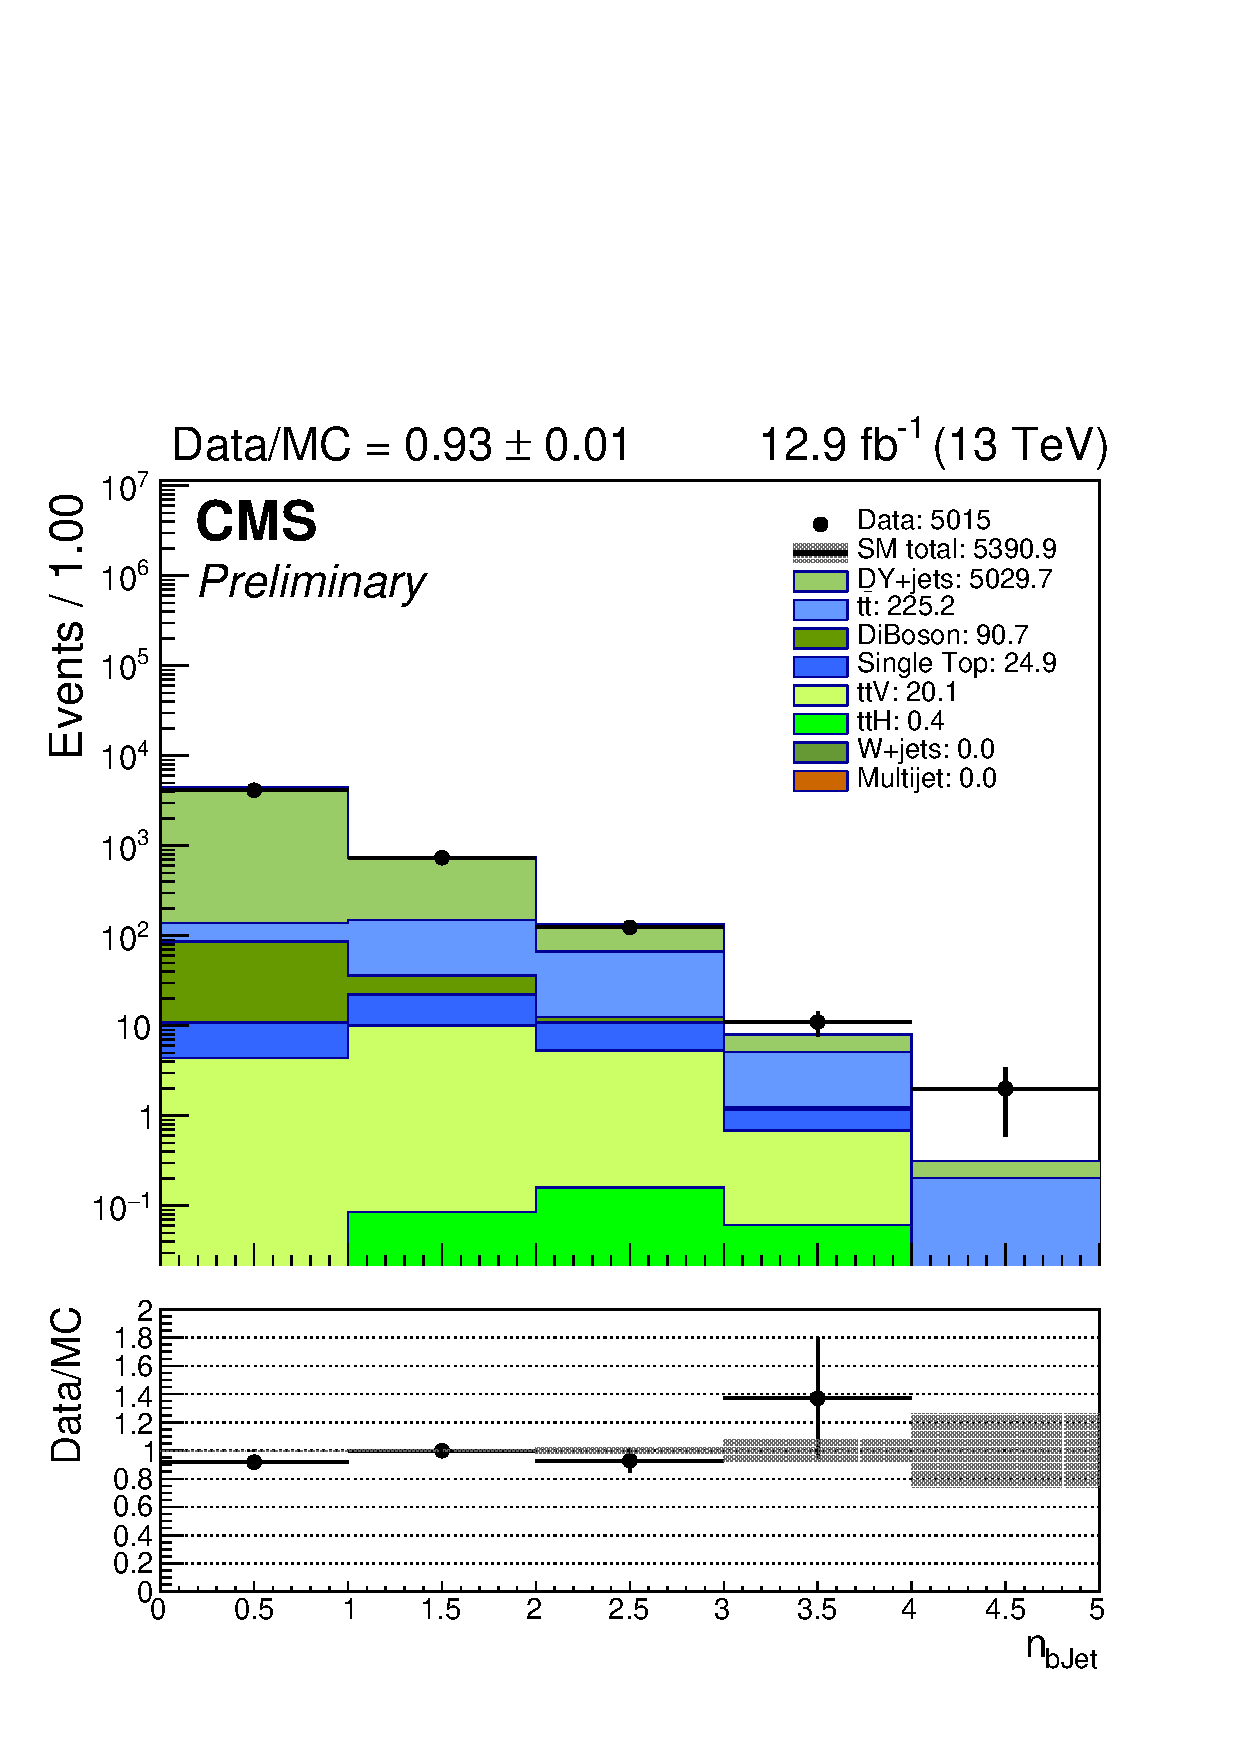
\includegraphics[width=0.5\textwidth]{figs/analysis/distributions/DoubleMu/nBJet40_sym.pdf}} \\
        \caption{Key analysis variables for double muon control region (symmetric \njet bins)}
        \label{fig:distribution_doublemu_sym}
    \end{center}
\end{figure}

\clearpage
\begin{figure}
    \begin{center}
        \subfloat {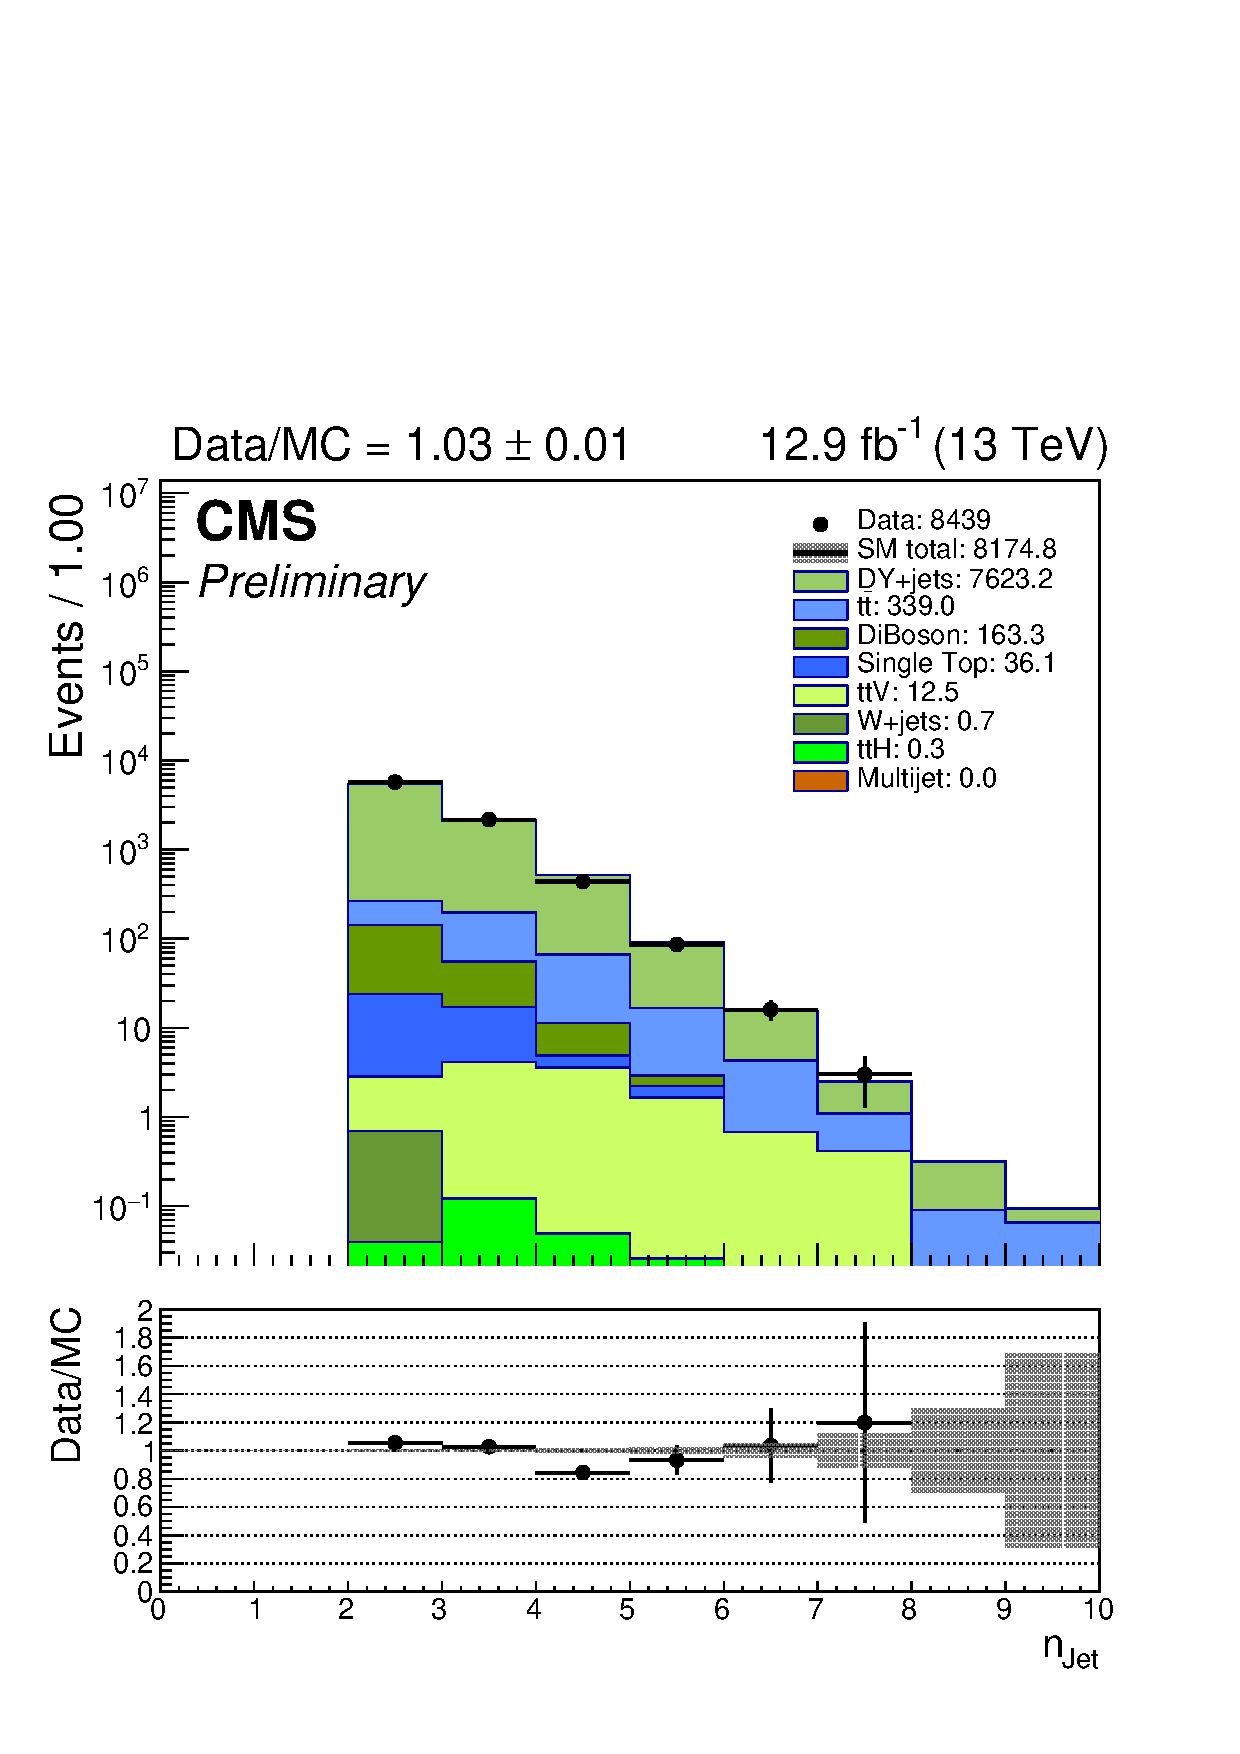
\includegraphics[width=0.5\textwidth]{figs/analysis/distributions/DoubleMu/nJet40_asym.pdf}} ~~
        \subfloat {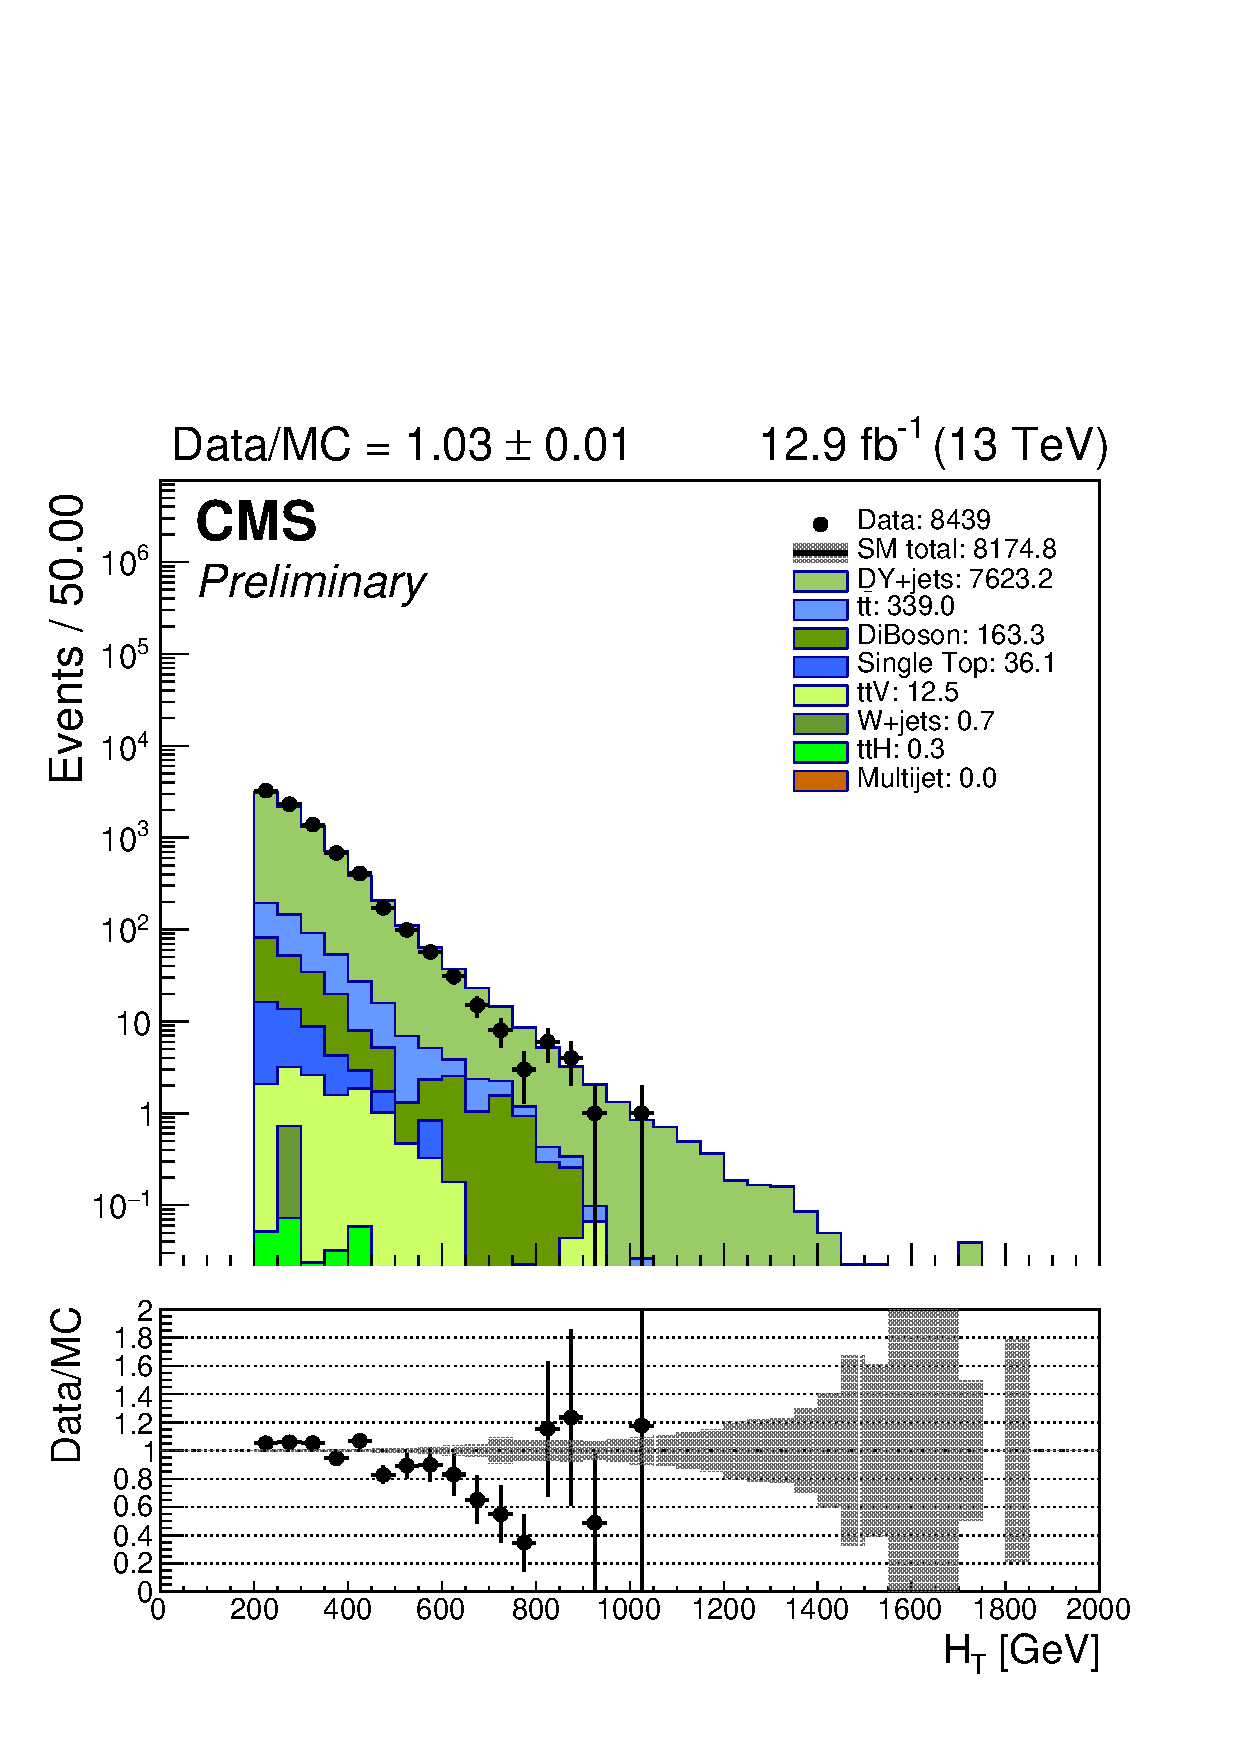
\includegraphics[width=0.5\textwidth]{figs/analysis/distributions/DoubleMu/ht40_asym.pdf}} \\
        \subfloat {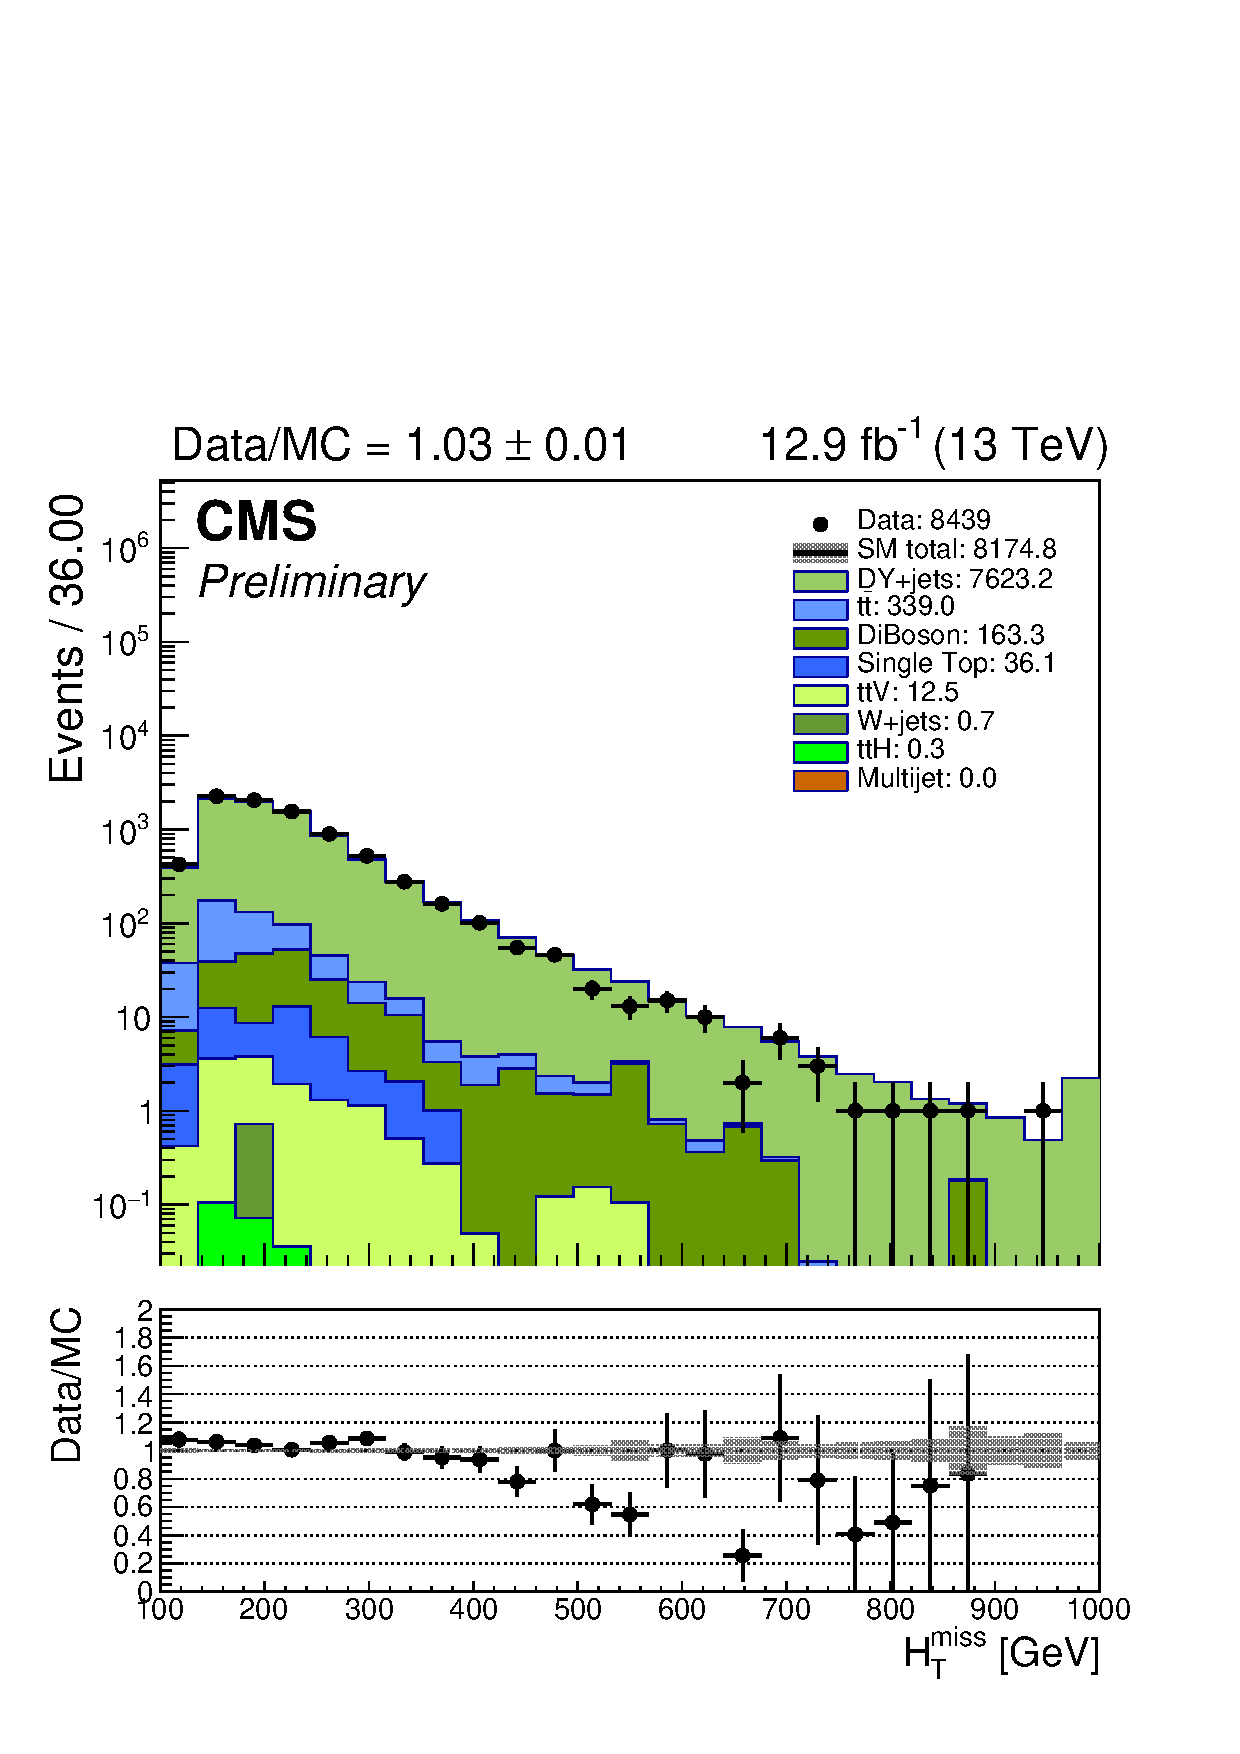
\includegraphics[width=0.5\textwidth]{figs/analysis/distributions/DoubleMu/mht40_pt_asym.pdf}} ~~
        \subfloat {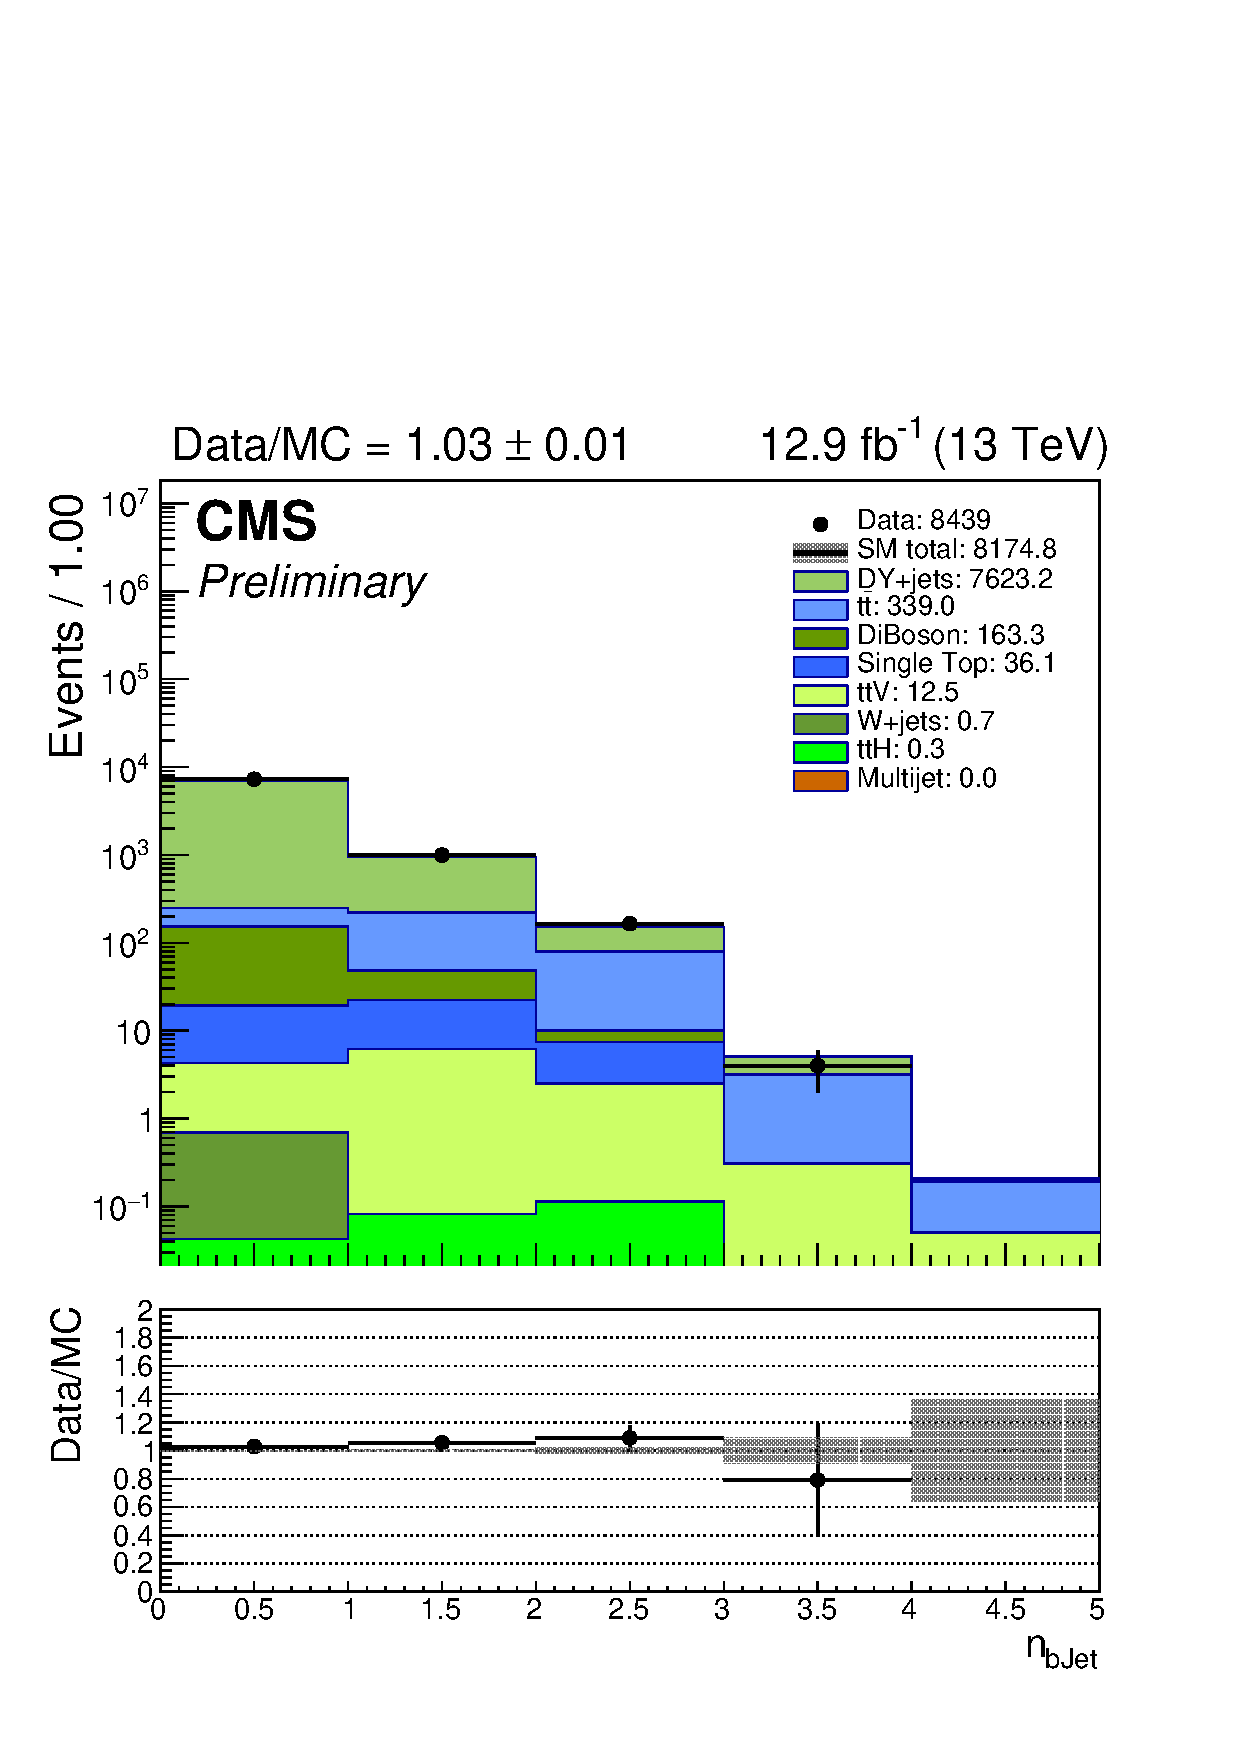
\includegraphics[width=0.5\textwidth]{figs/analysis/distributions/DoubleMu/nBJet40_asym.pdf}} \\
        \caption{Key analysis variables for double muon control region (asymmetric \njet bins)}
        \label{fig:distribution_doublemu_asym}
    \end{center}
\end{figure}

\begin{figure}
    \begin{center} 
        \subfloat {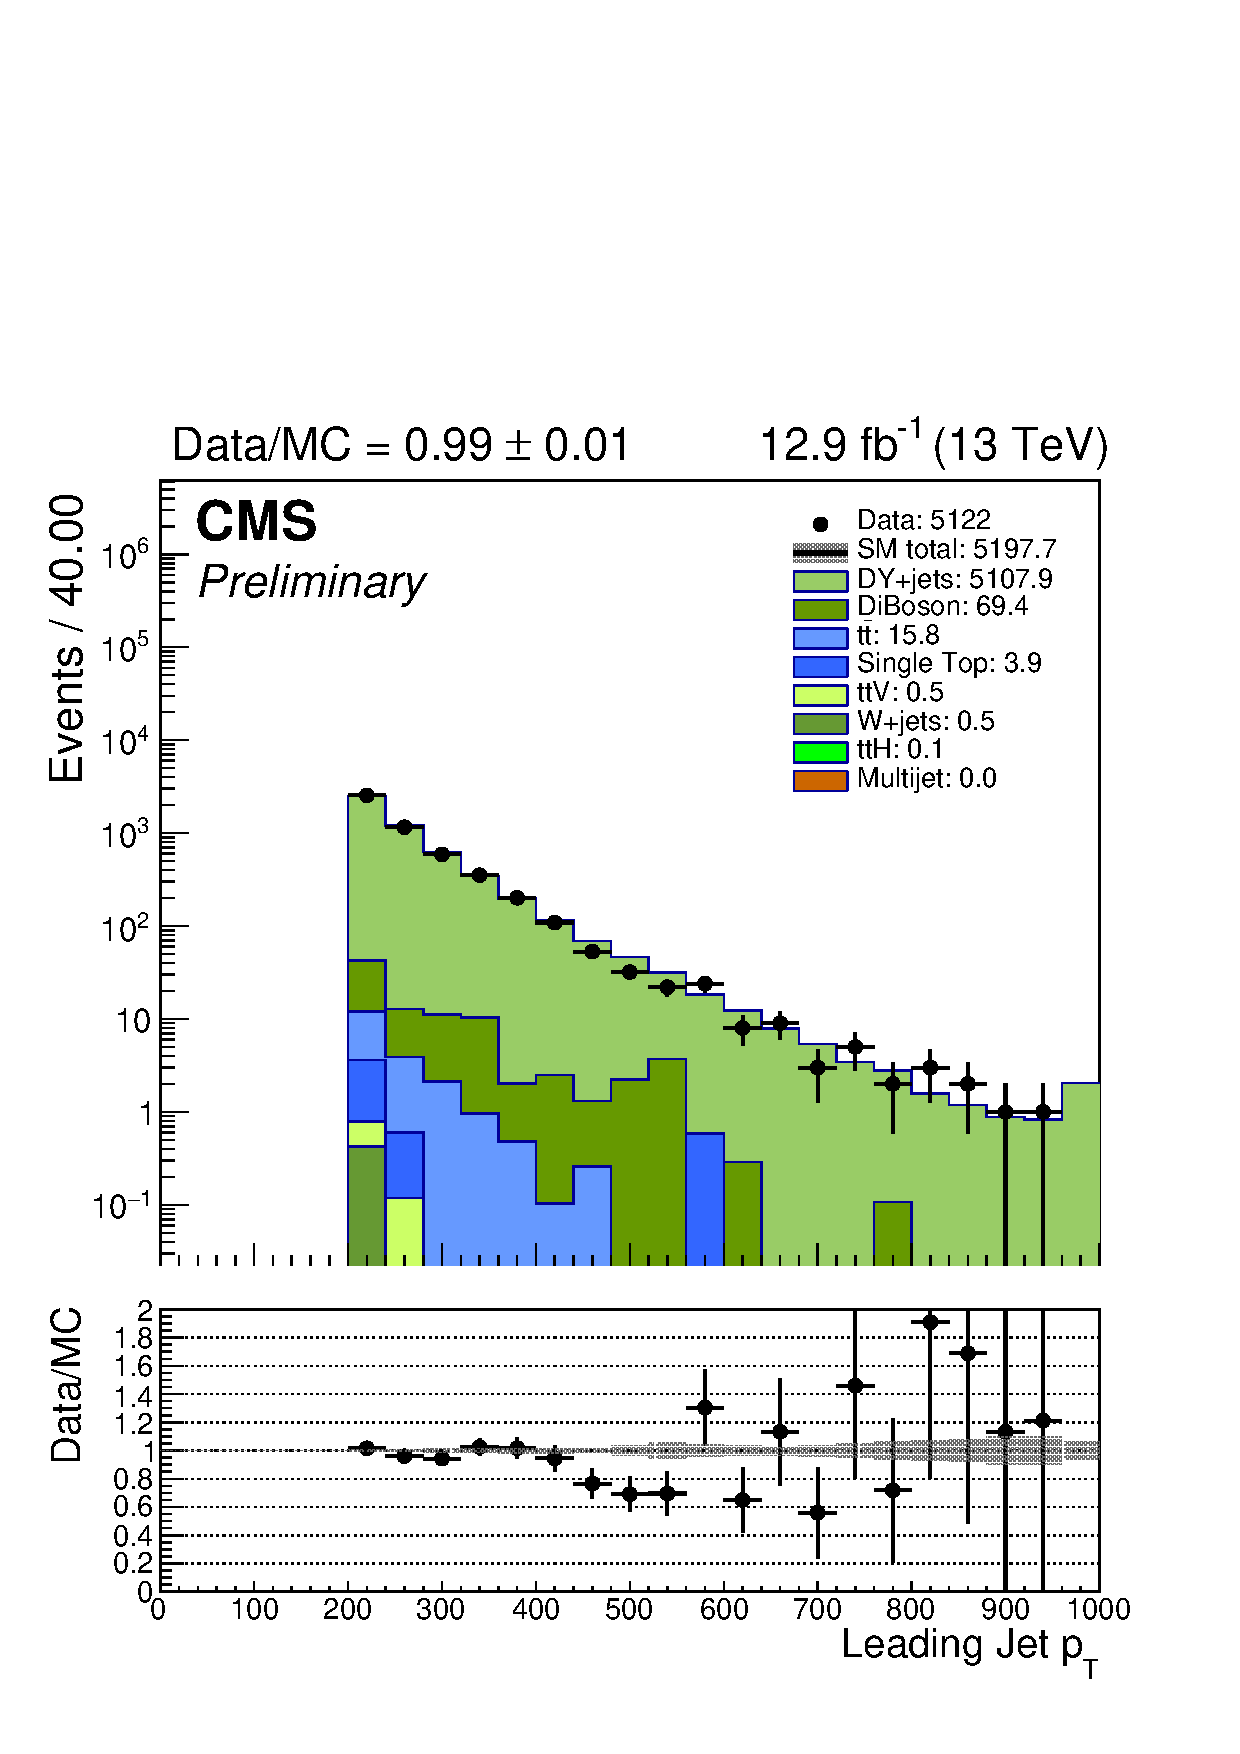
\includegraphics[width=0.5\textwidth]{figs/analysis/distributions/DoubleMu/jet_pt[0]_eq1j.pdf}} ~~
        \subfloat {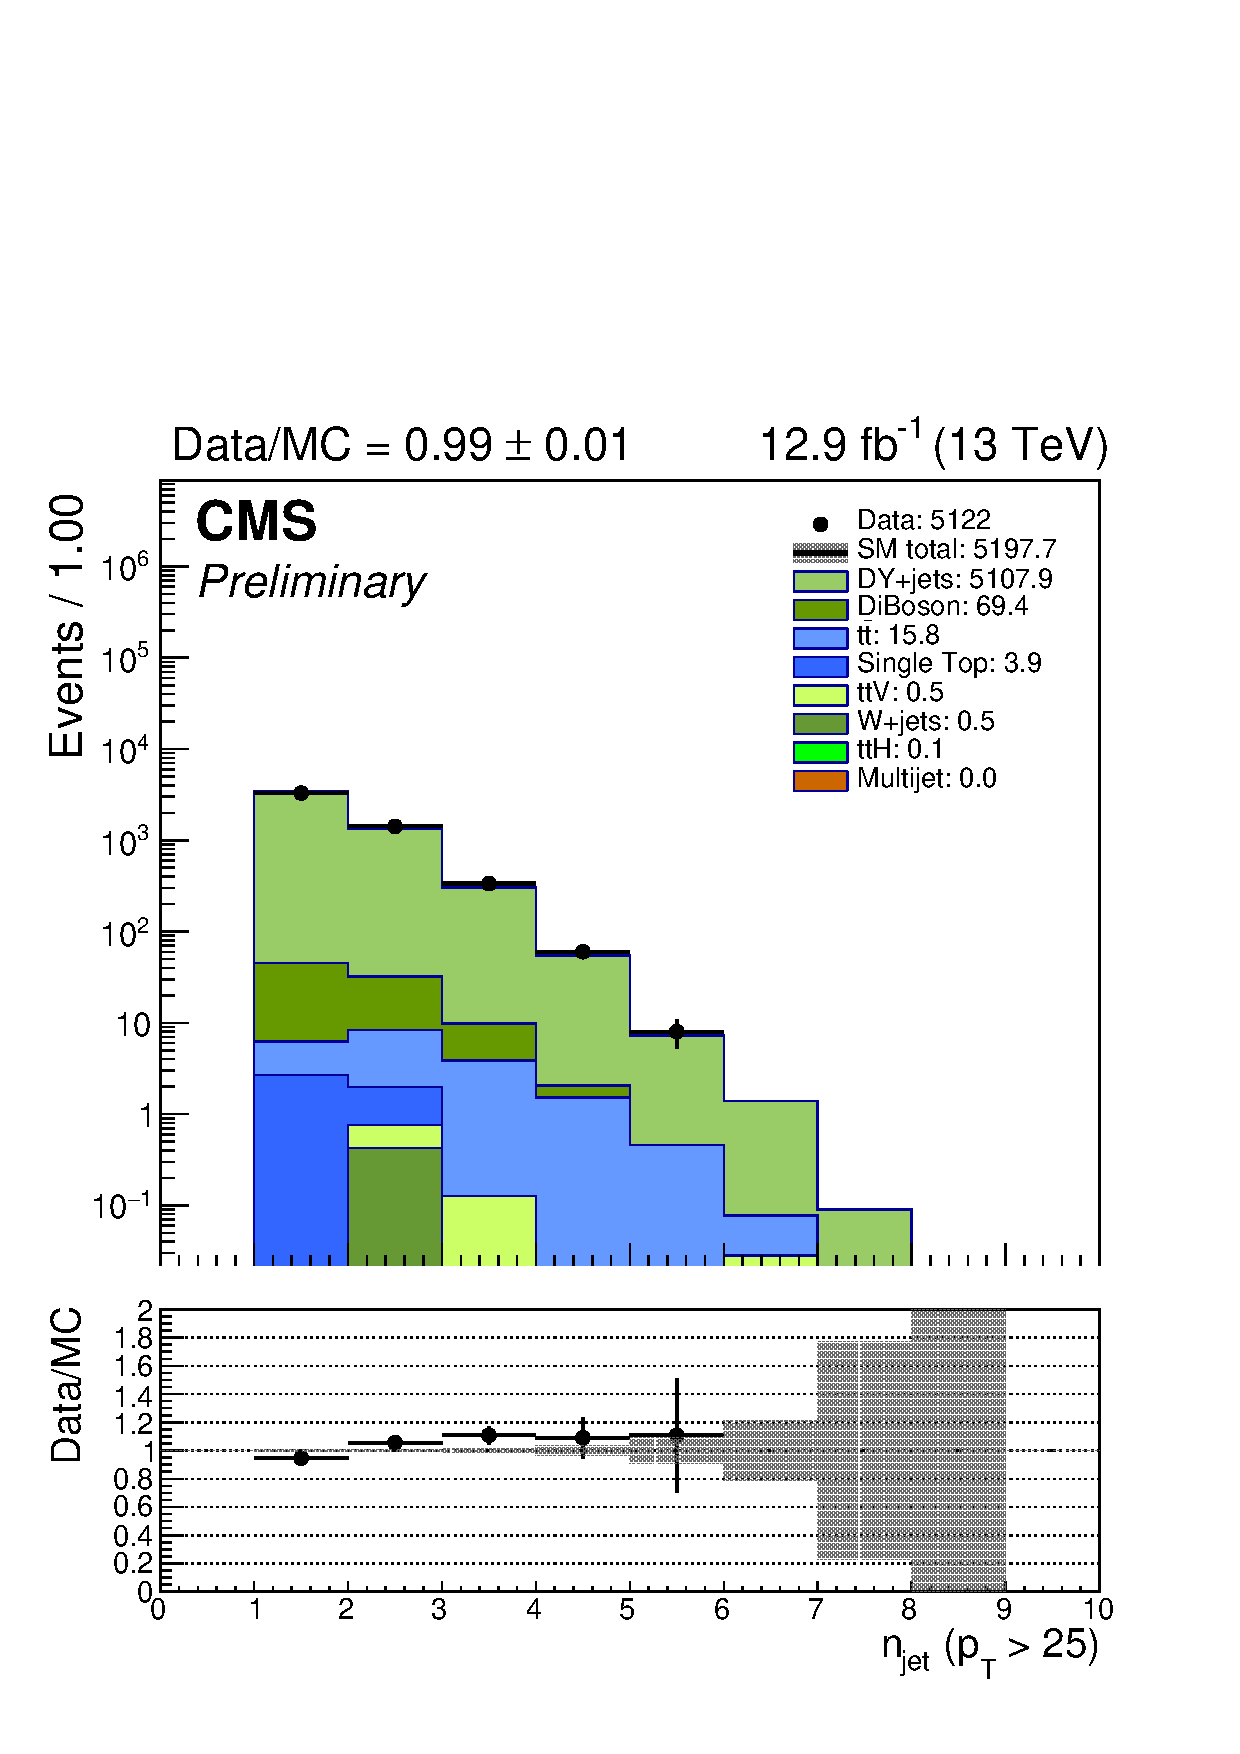
\includegraphics[width=0.5\textwidth]{figs/analysis/distributions/DoubleMu/njetInc_eq1j.pdf}} \\
        \subfloat {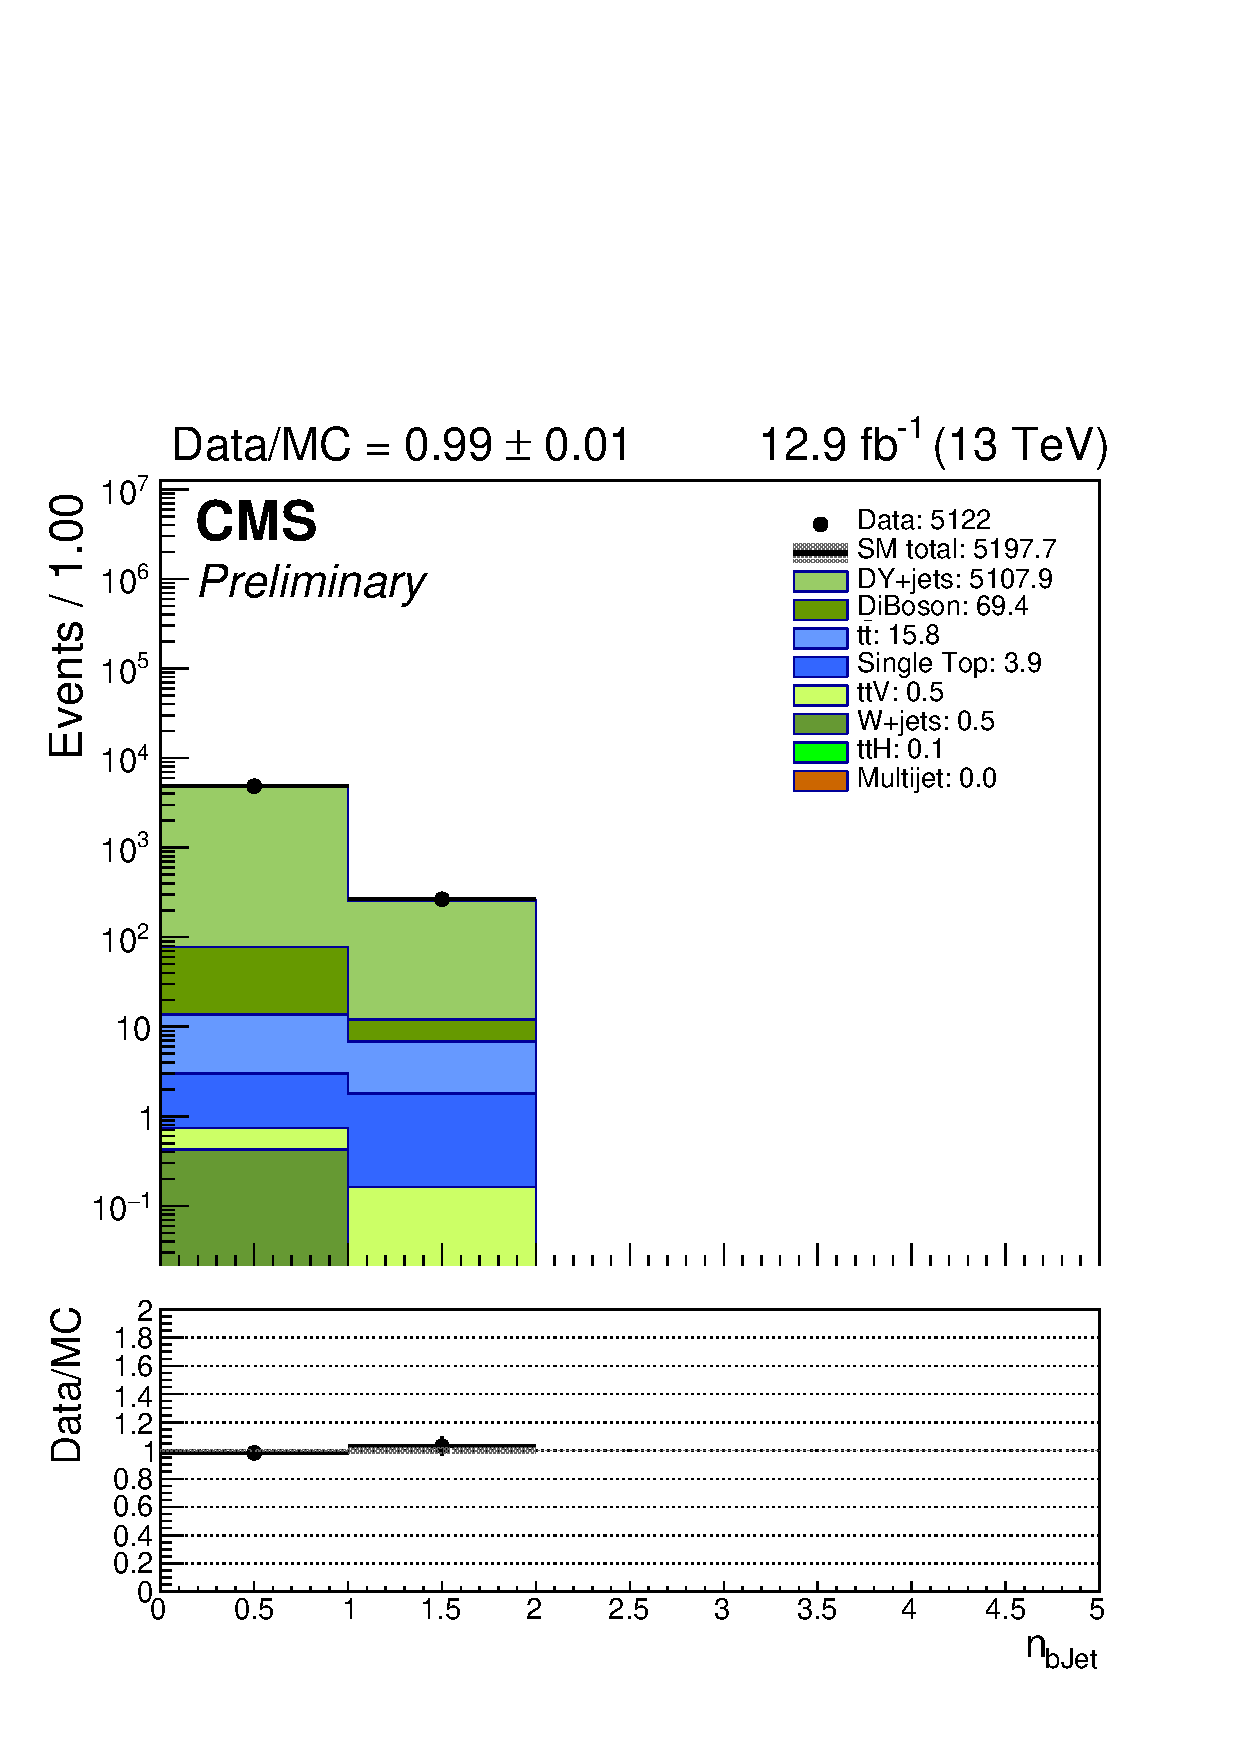
\includegraphics[width=0.5\textwidth]{figs/analysis/distributions/DoubleMu/nBJet40_eq1j.pdf}} ~~
        \subfloat {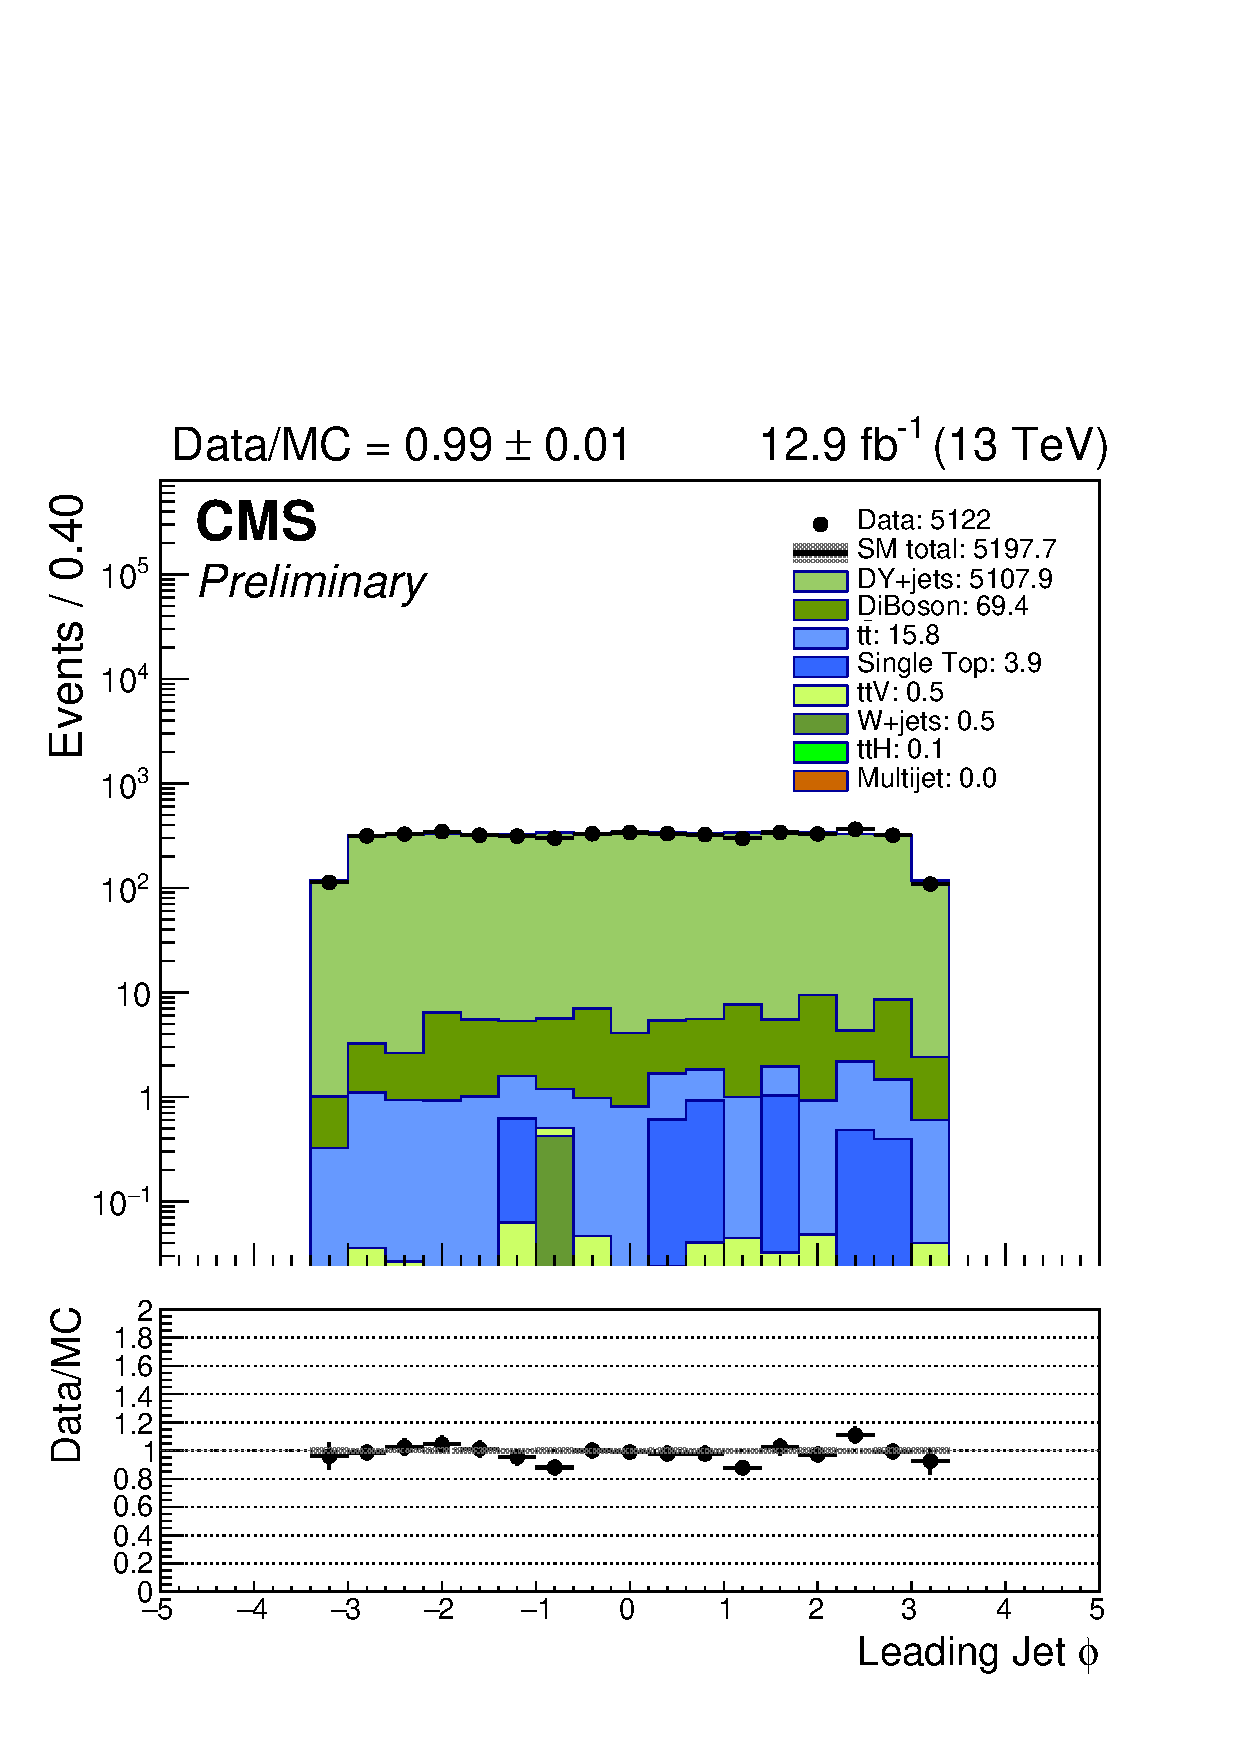
\includegraphics[width=0.5\textwidth]{figs/analysis/distributions/DoubleMu/jet_phi[0]_eq1j.pdf}} \\
        \caption{Key analysis variables for double muon control region (monojet bins)}
        \label{fig:distribution_doublemu_mono}
    \end{center}
\end{figure}

% \clearpage
% \subsection{Yields and distributions for the photon + jets control sample}

\begin{figure}
    \begin{center}
        \subfloat {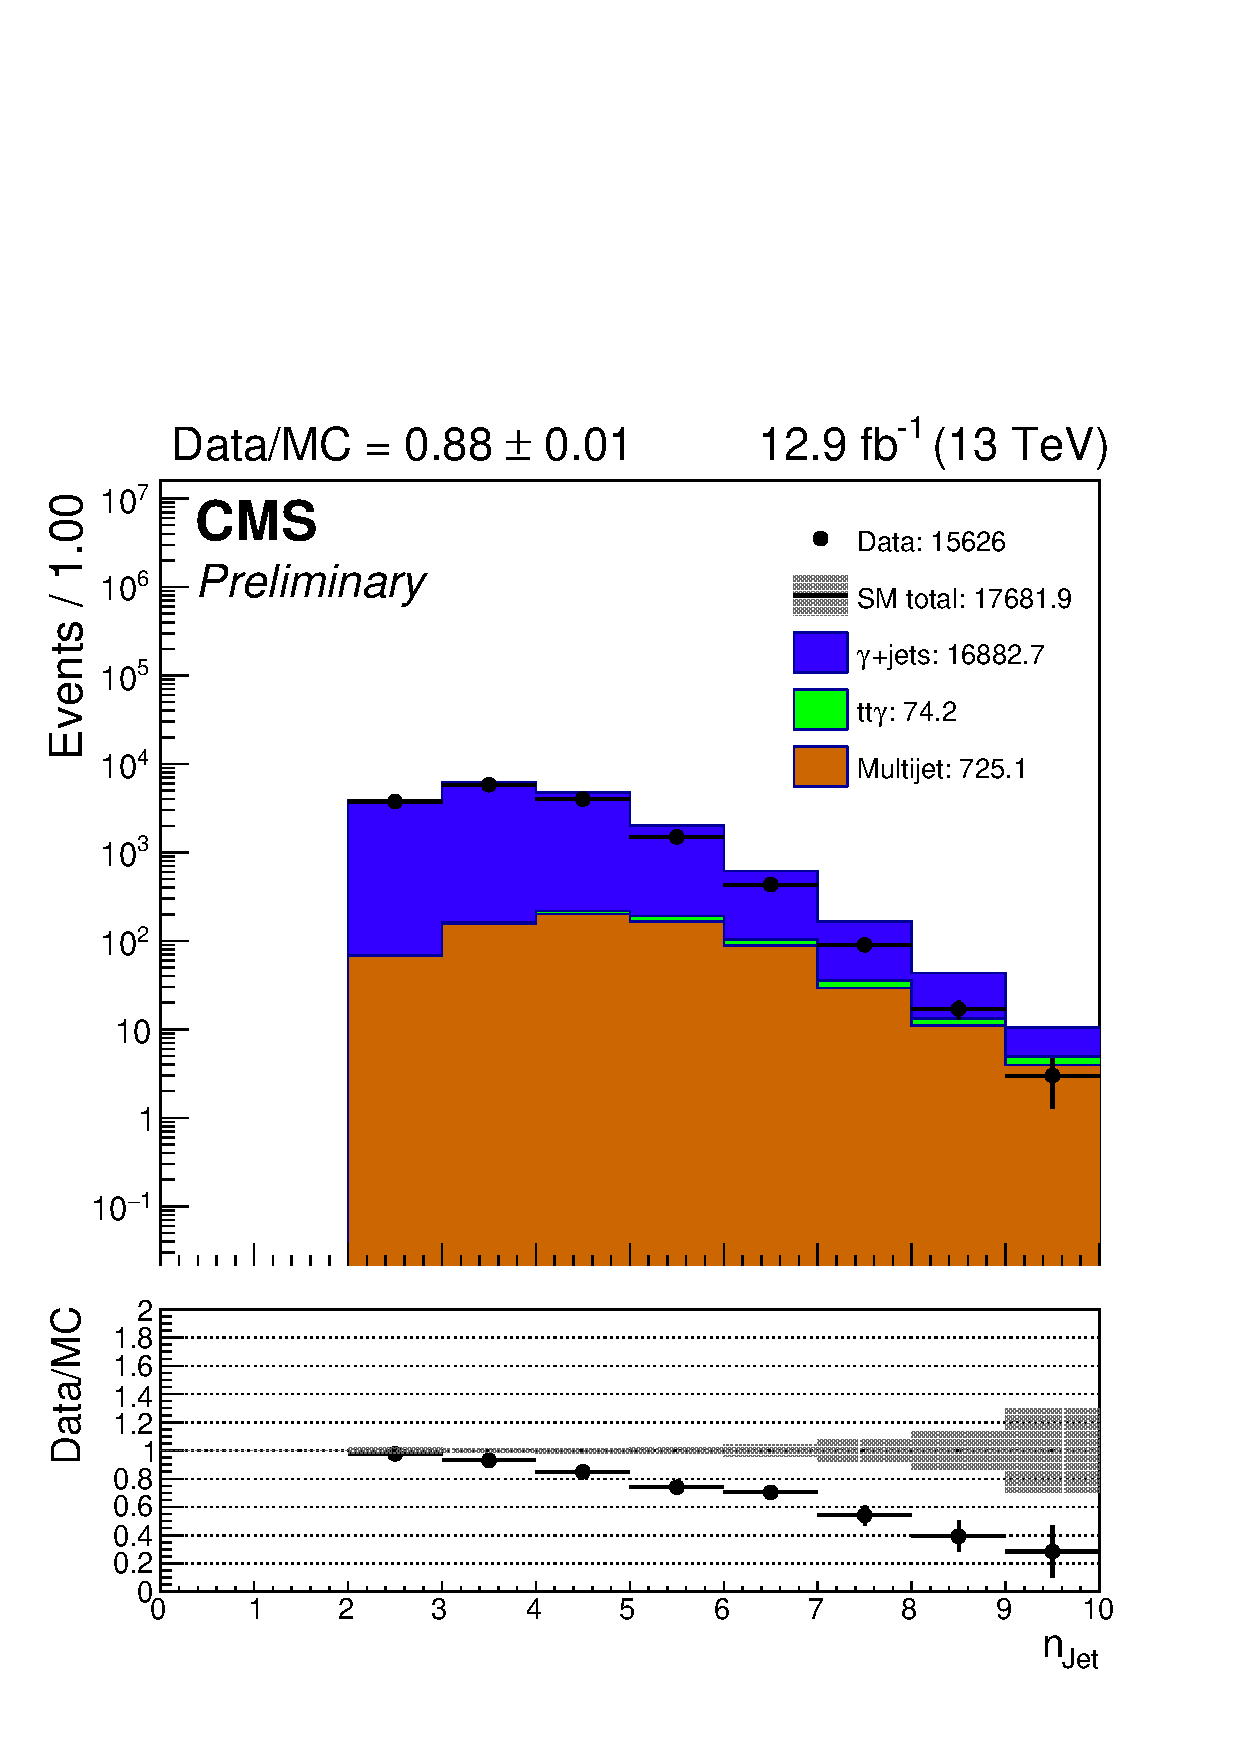
\includegraphics[width=0.5\textwidth]{figs/analysis/distributions/SinglePhoton/nJet40_sym.pdf}} ~~
        \subfloat {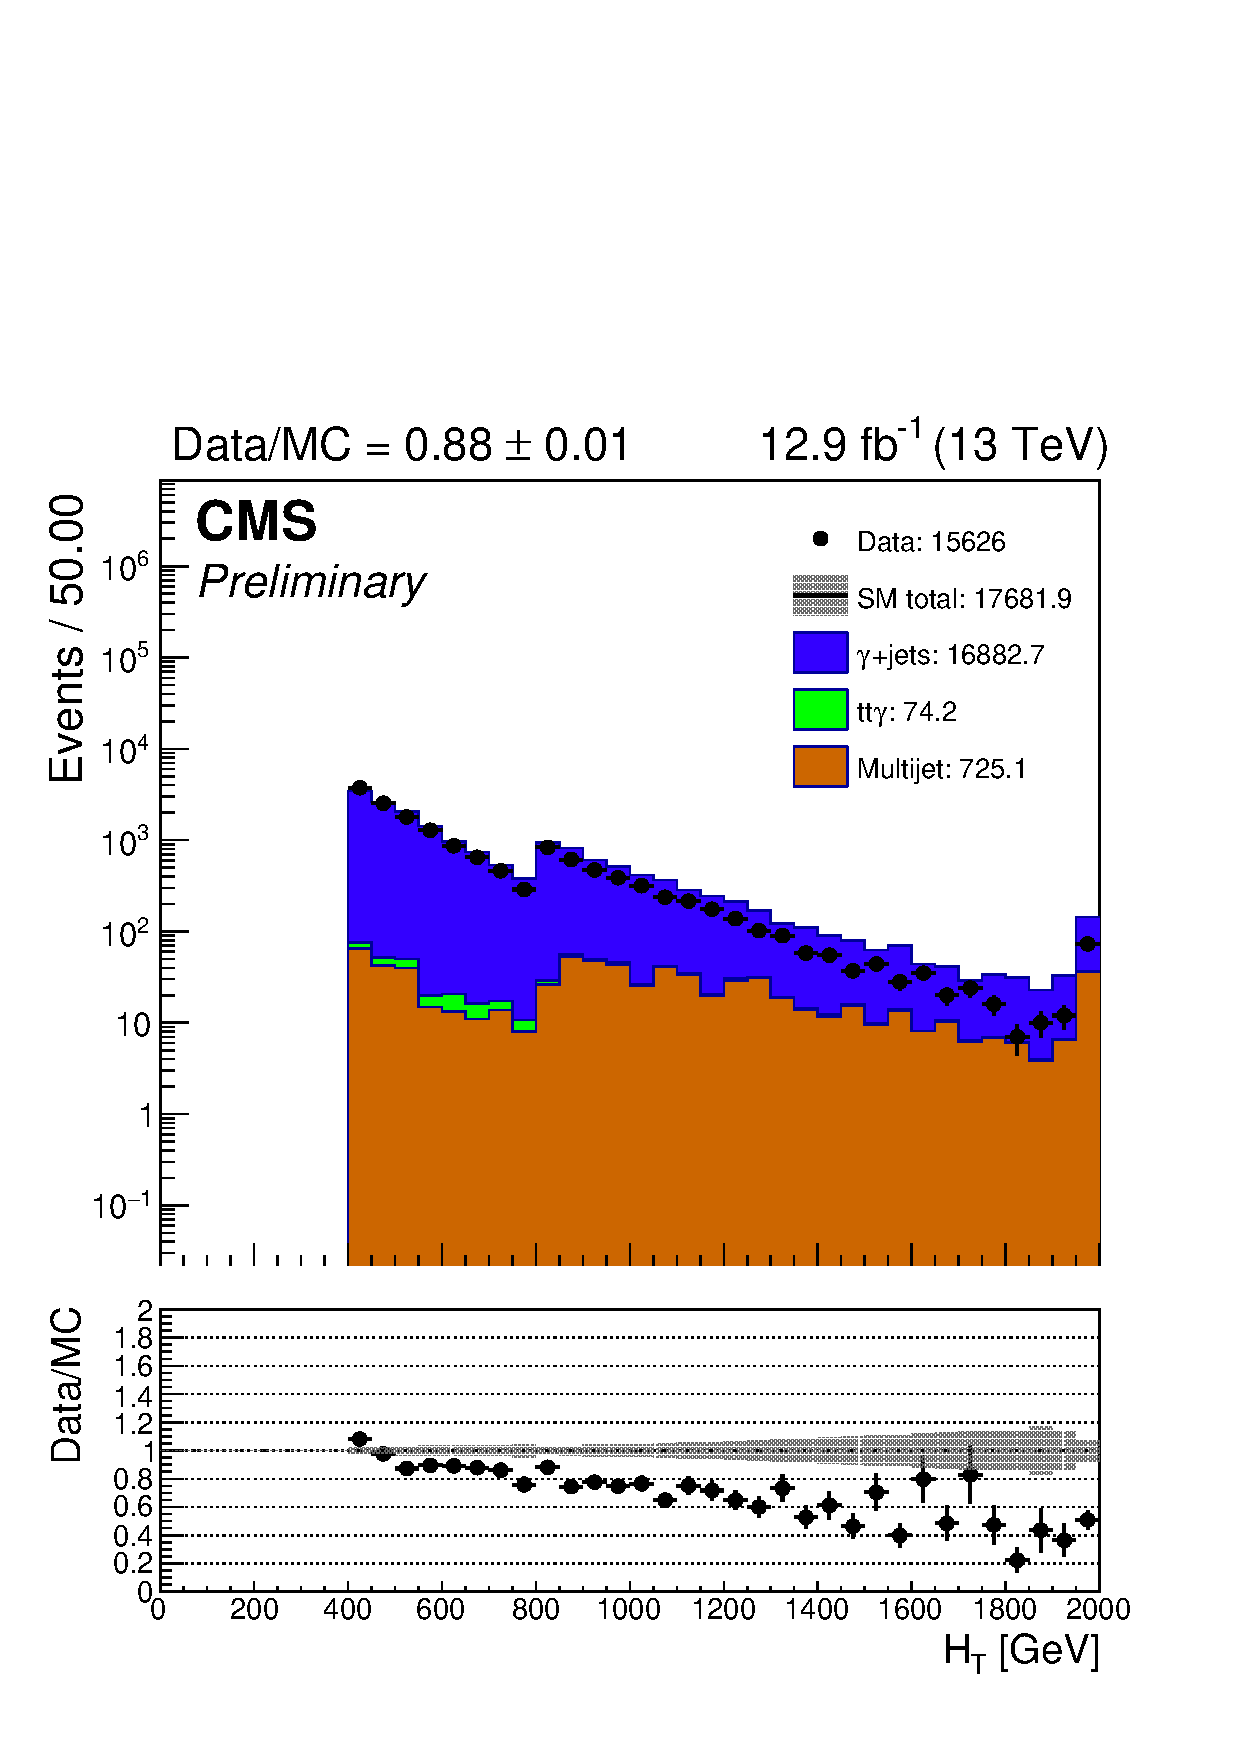
\includegraphics[width=0.5\textwidth]{figs/analysis/distributions/SinglePhoton/ht40_sym.pdf}} \\
        \subfloat {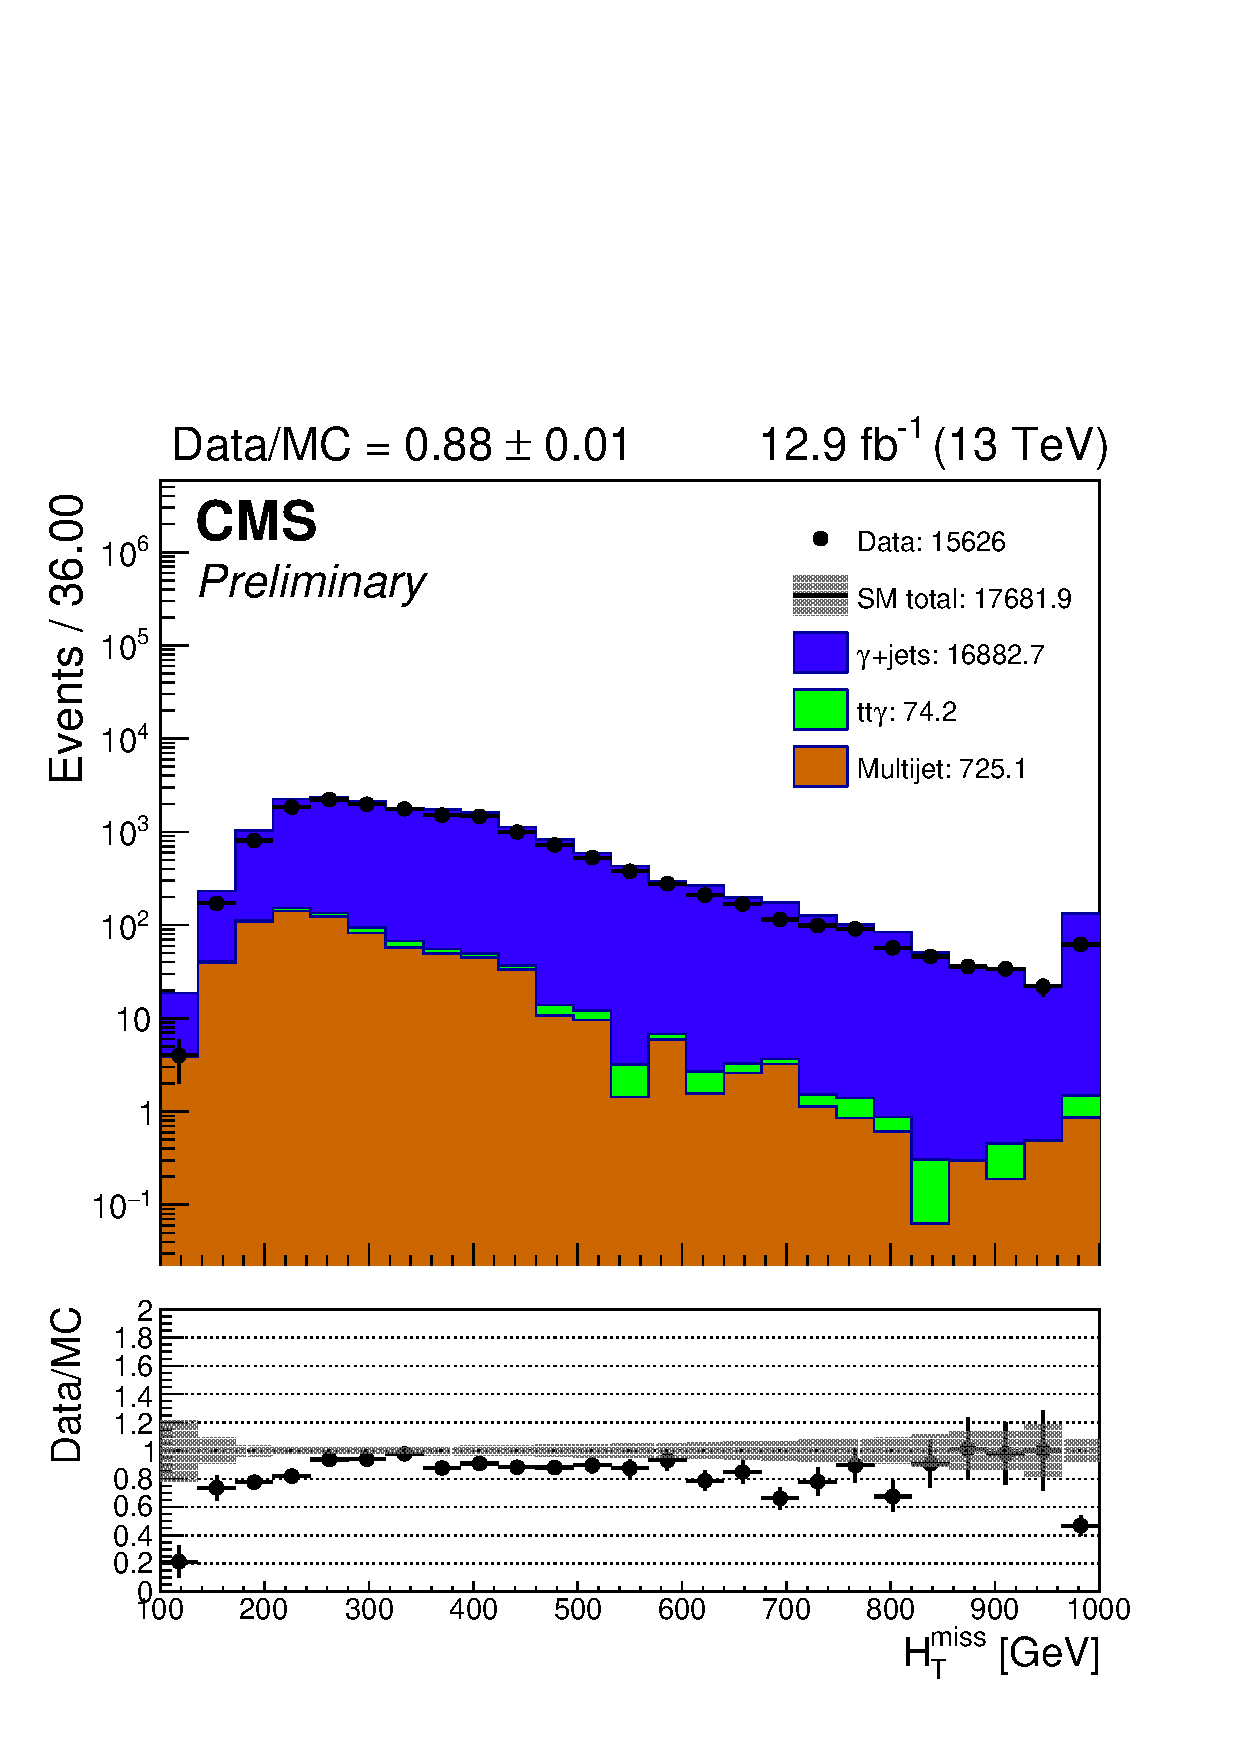
\includegraphics[width=0.5\textwidth]{figs/analysis/distributions/SinglePhoton/mht40_pt_sym.pdf}} ~~
        \subfloat {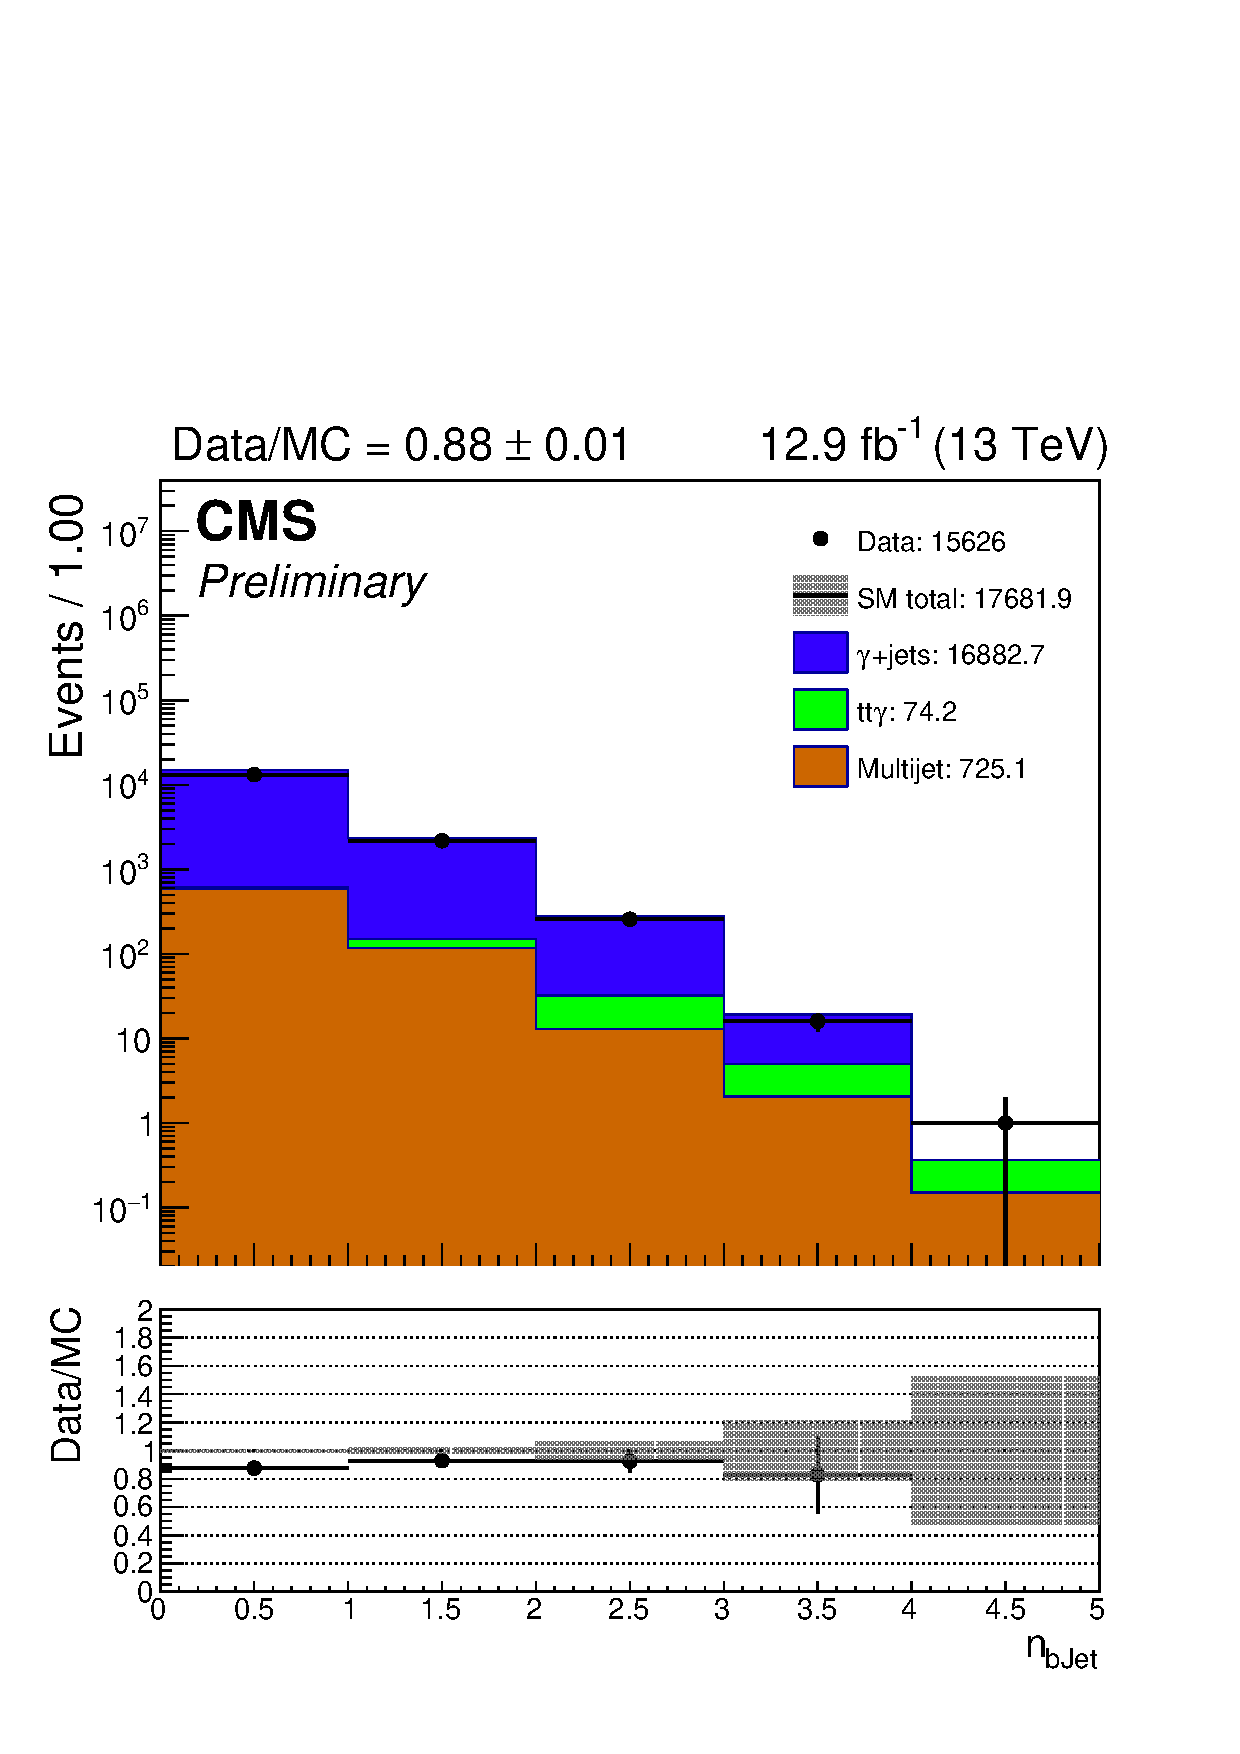
\includegraphics[width=0.5\textwidth]{figs/analysis/distributions/SinglePhoton/nBJet40_sym.pdf}} \\
        \caption{Key analysis variables for single photon control region (symmetric \njet bins)}
        \label{fig:distribution_singlephoton_sym}
    \end{center}
\end{figure}

\clearpage
\begin{figure}[h]
    \begin{center}
        \subfloat {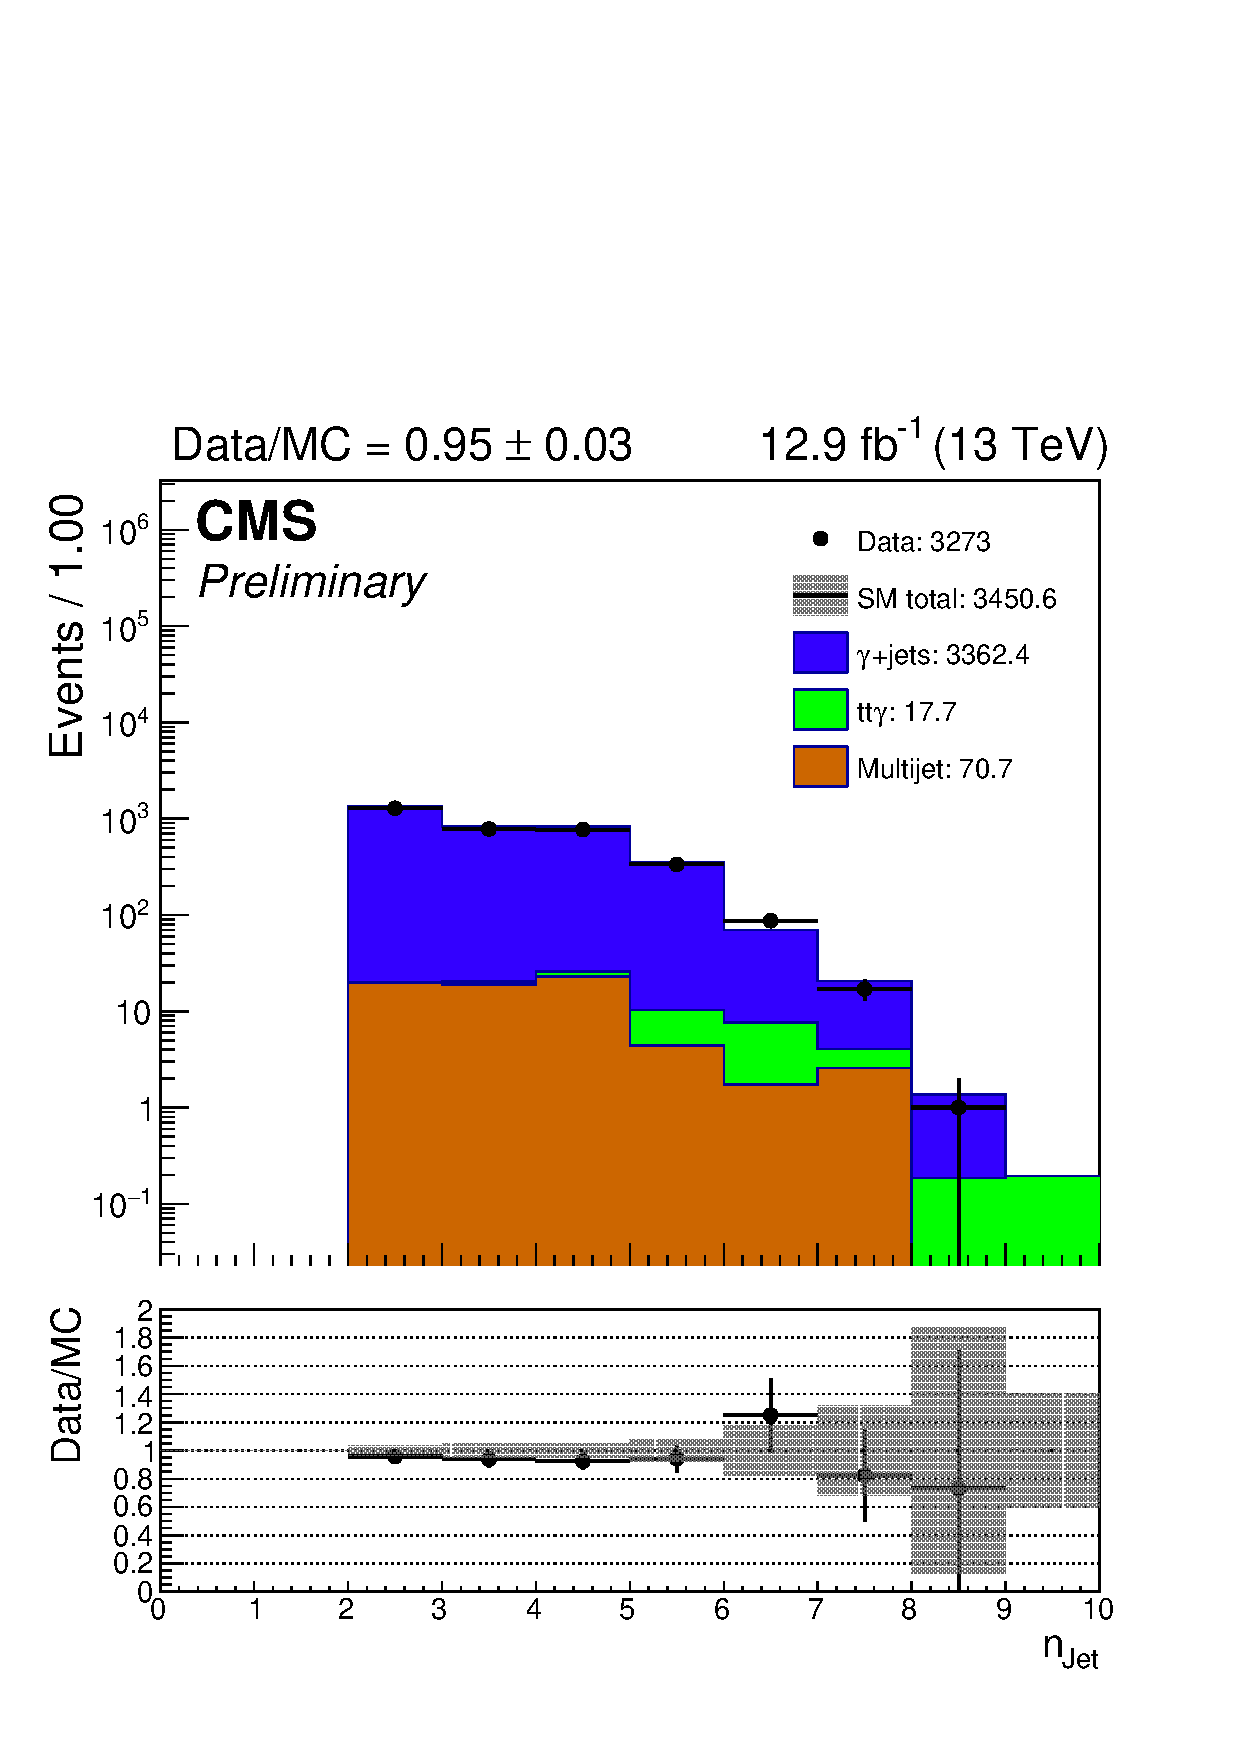
\includegraphics[width=0.5\textwidth]{figs/analysis/distributions/SinglePhoton/nJet40_asym.pdf}} ~~
        \subfloat {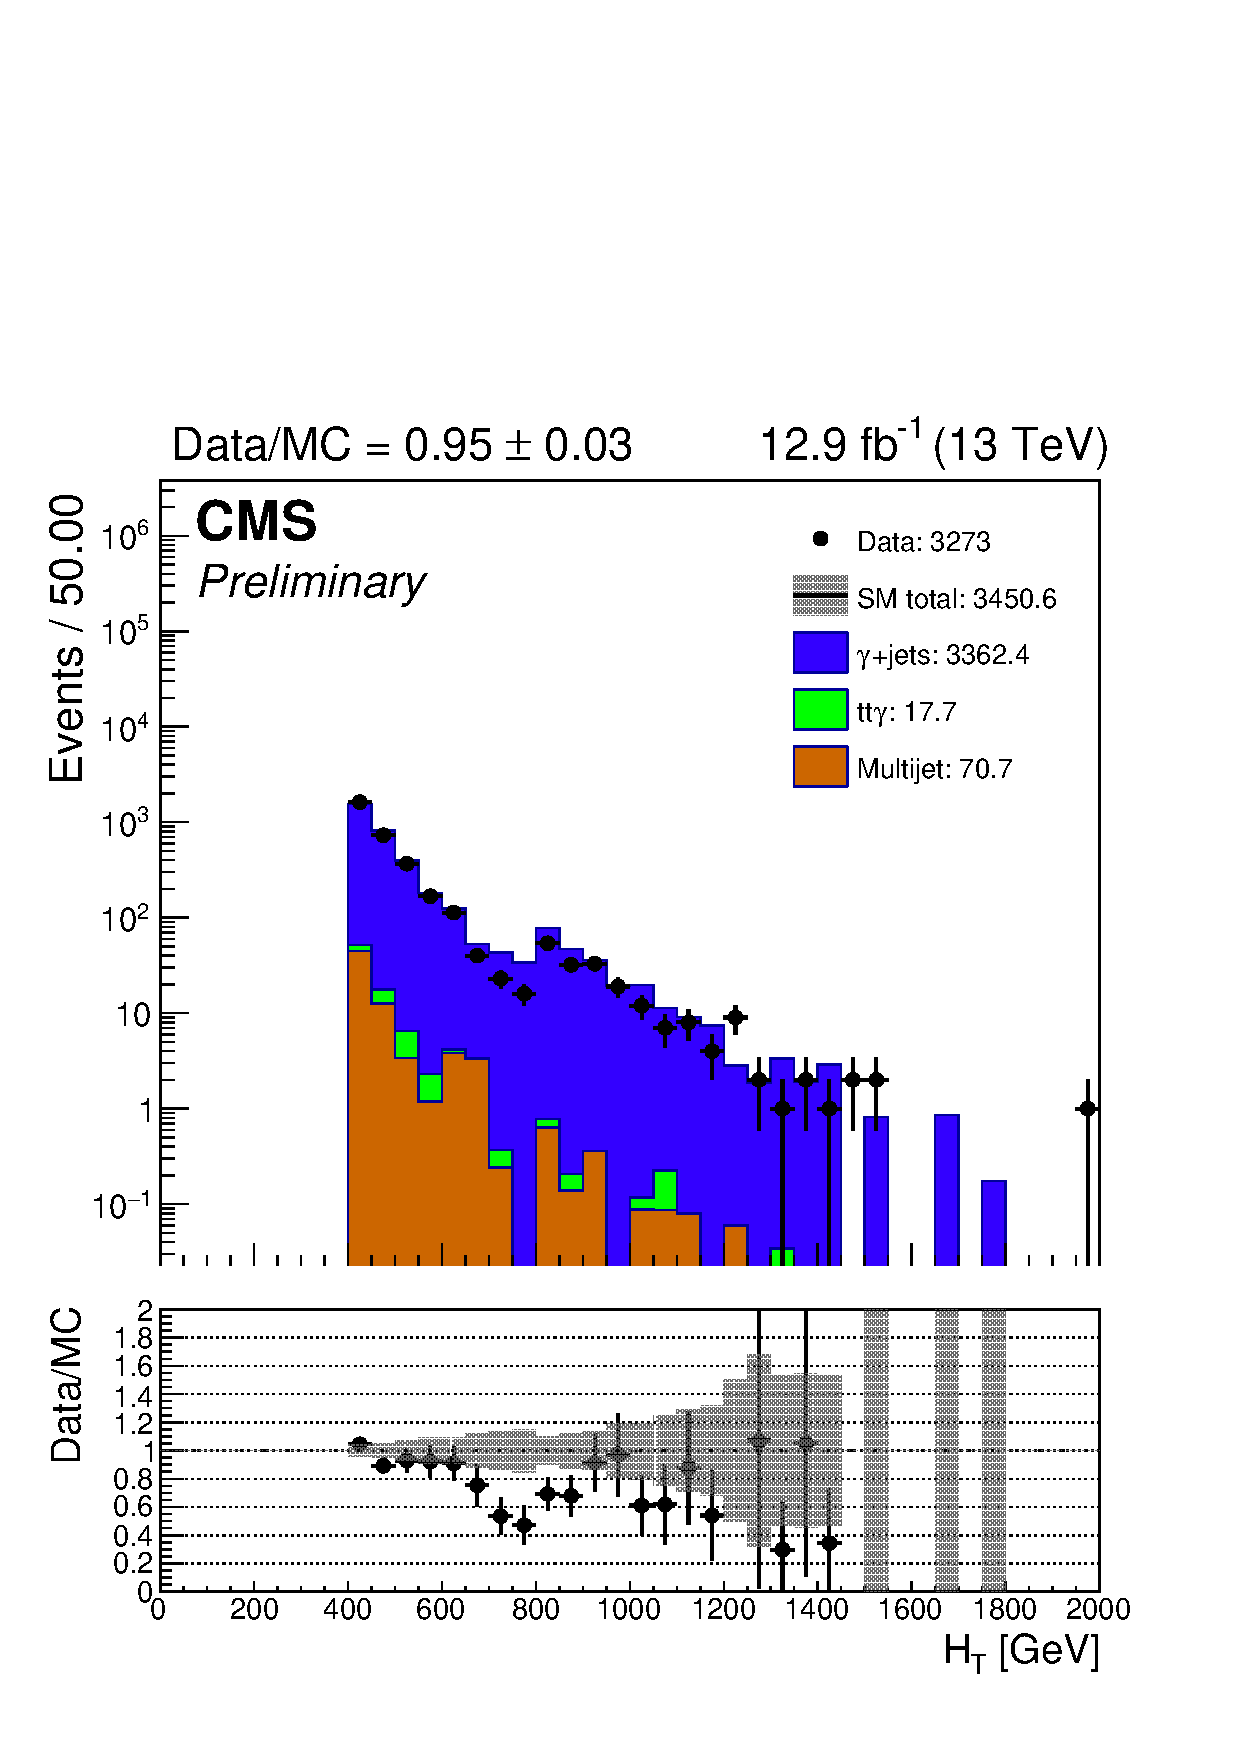
\includegraphics[width=0.5\textwidth]{figs/analysis/distributions/SinglePhoton/ht40_asym.pdf}} \\
        \subfloat {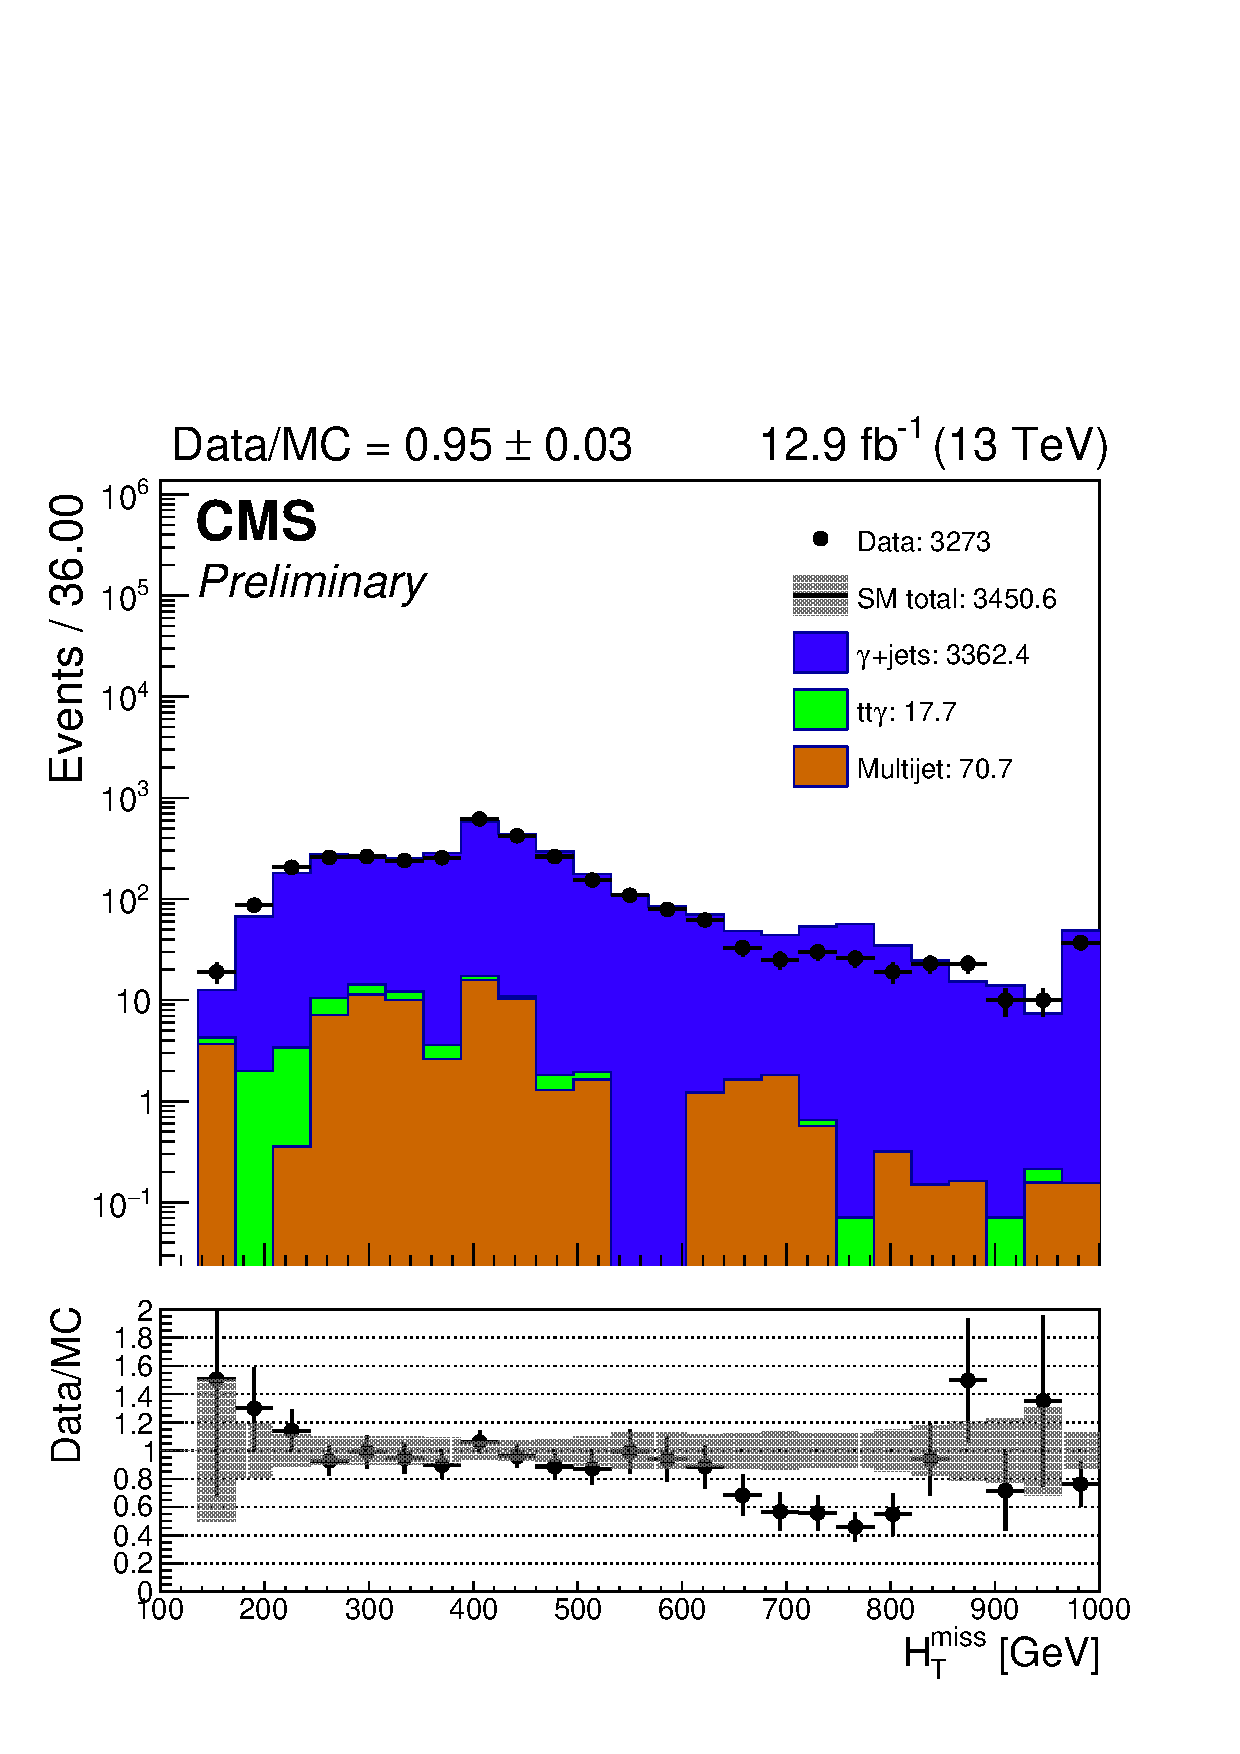
\includegraphics[width=0.5\textwidth]{figs/analysis/distributions/SinglePhoton/mht40_pt_asym.pdf}} ~~
        \subfloat {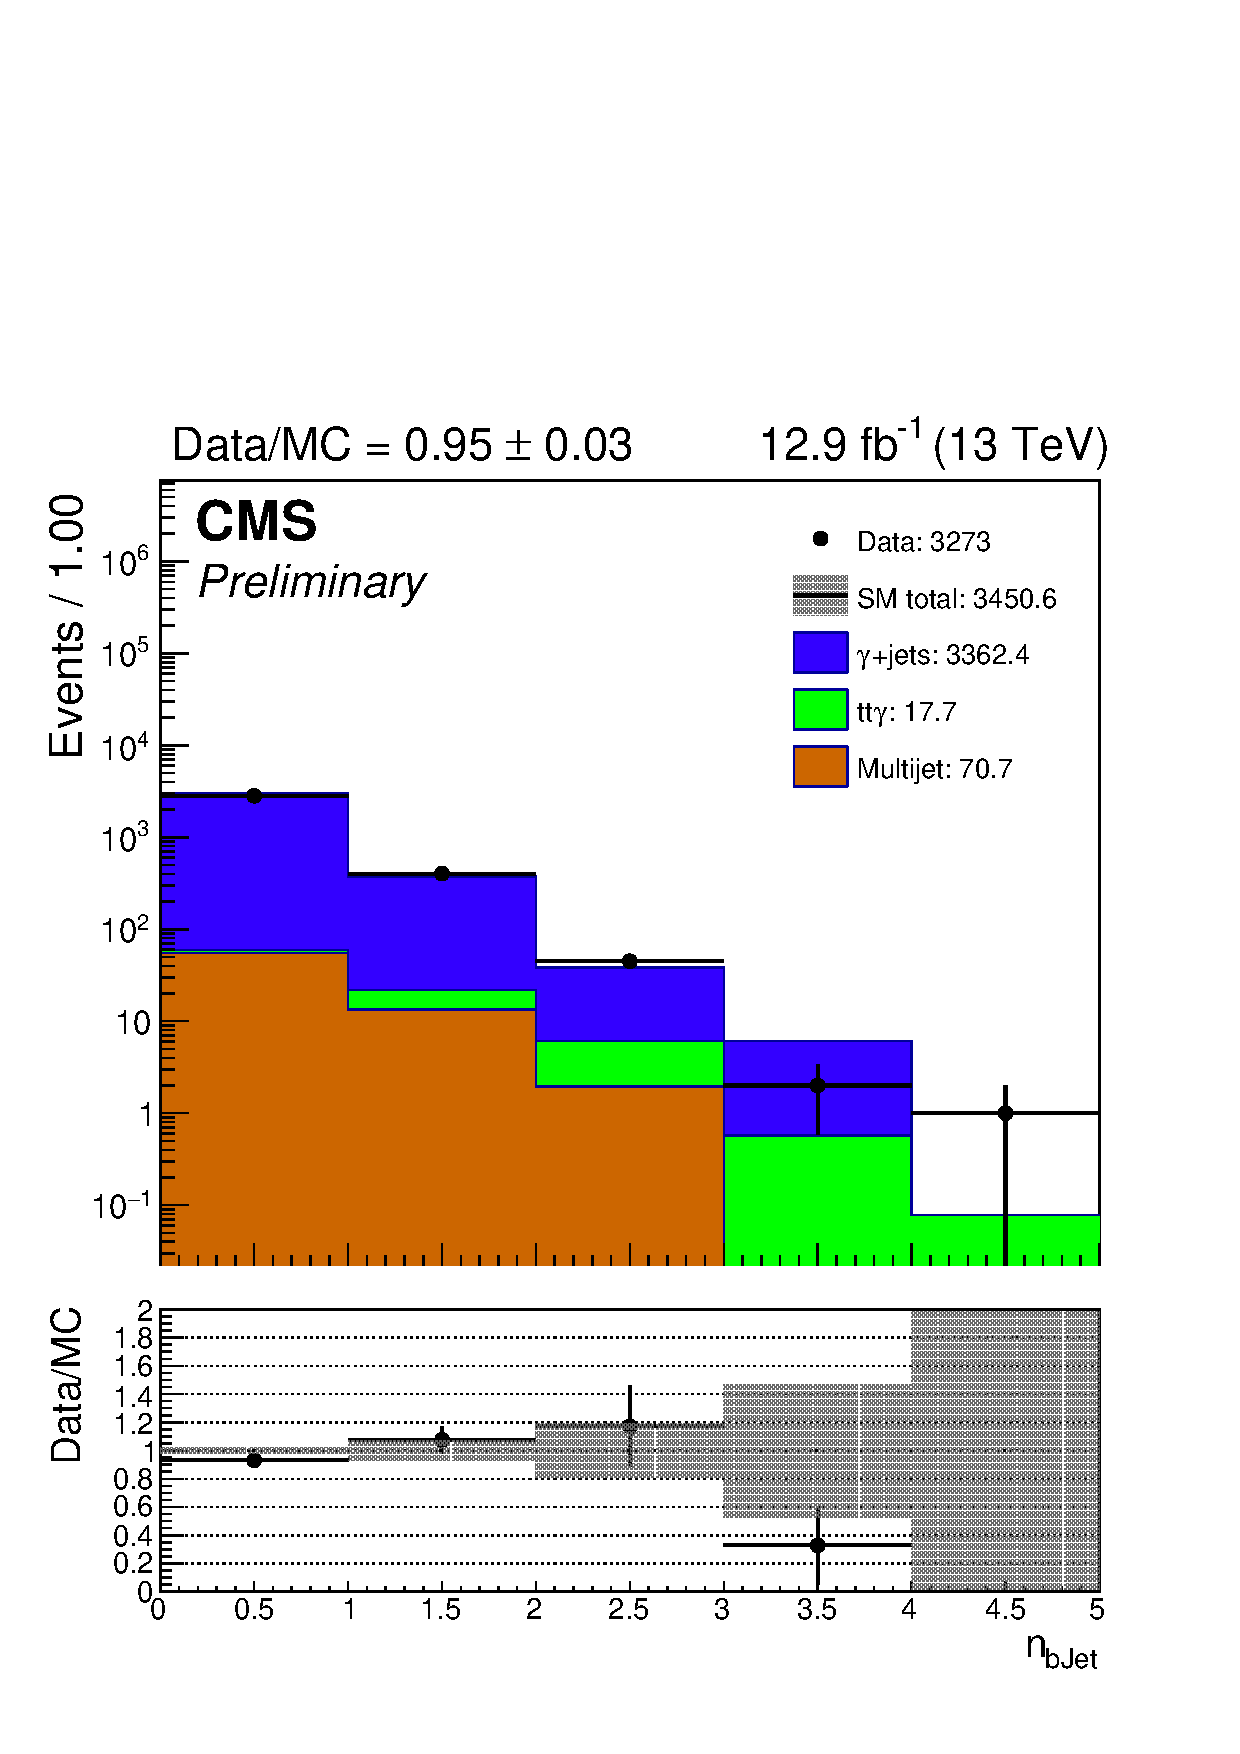
\includegraphics[width=0.5\textwidth]{figs/analysis/distributions/SinglePhoton/nBJet40_asym.pdf}} \\
        \caption{Key analysis variables for single photon control region (asymmetric \njet bins)}
        \label{fig:distribution_singlephoton_asym}
    \end{center}
\end{figure}

\clearpage
\begin{figure}
    \begin{center} 
        \subfloat {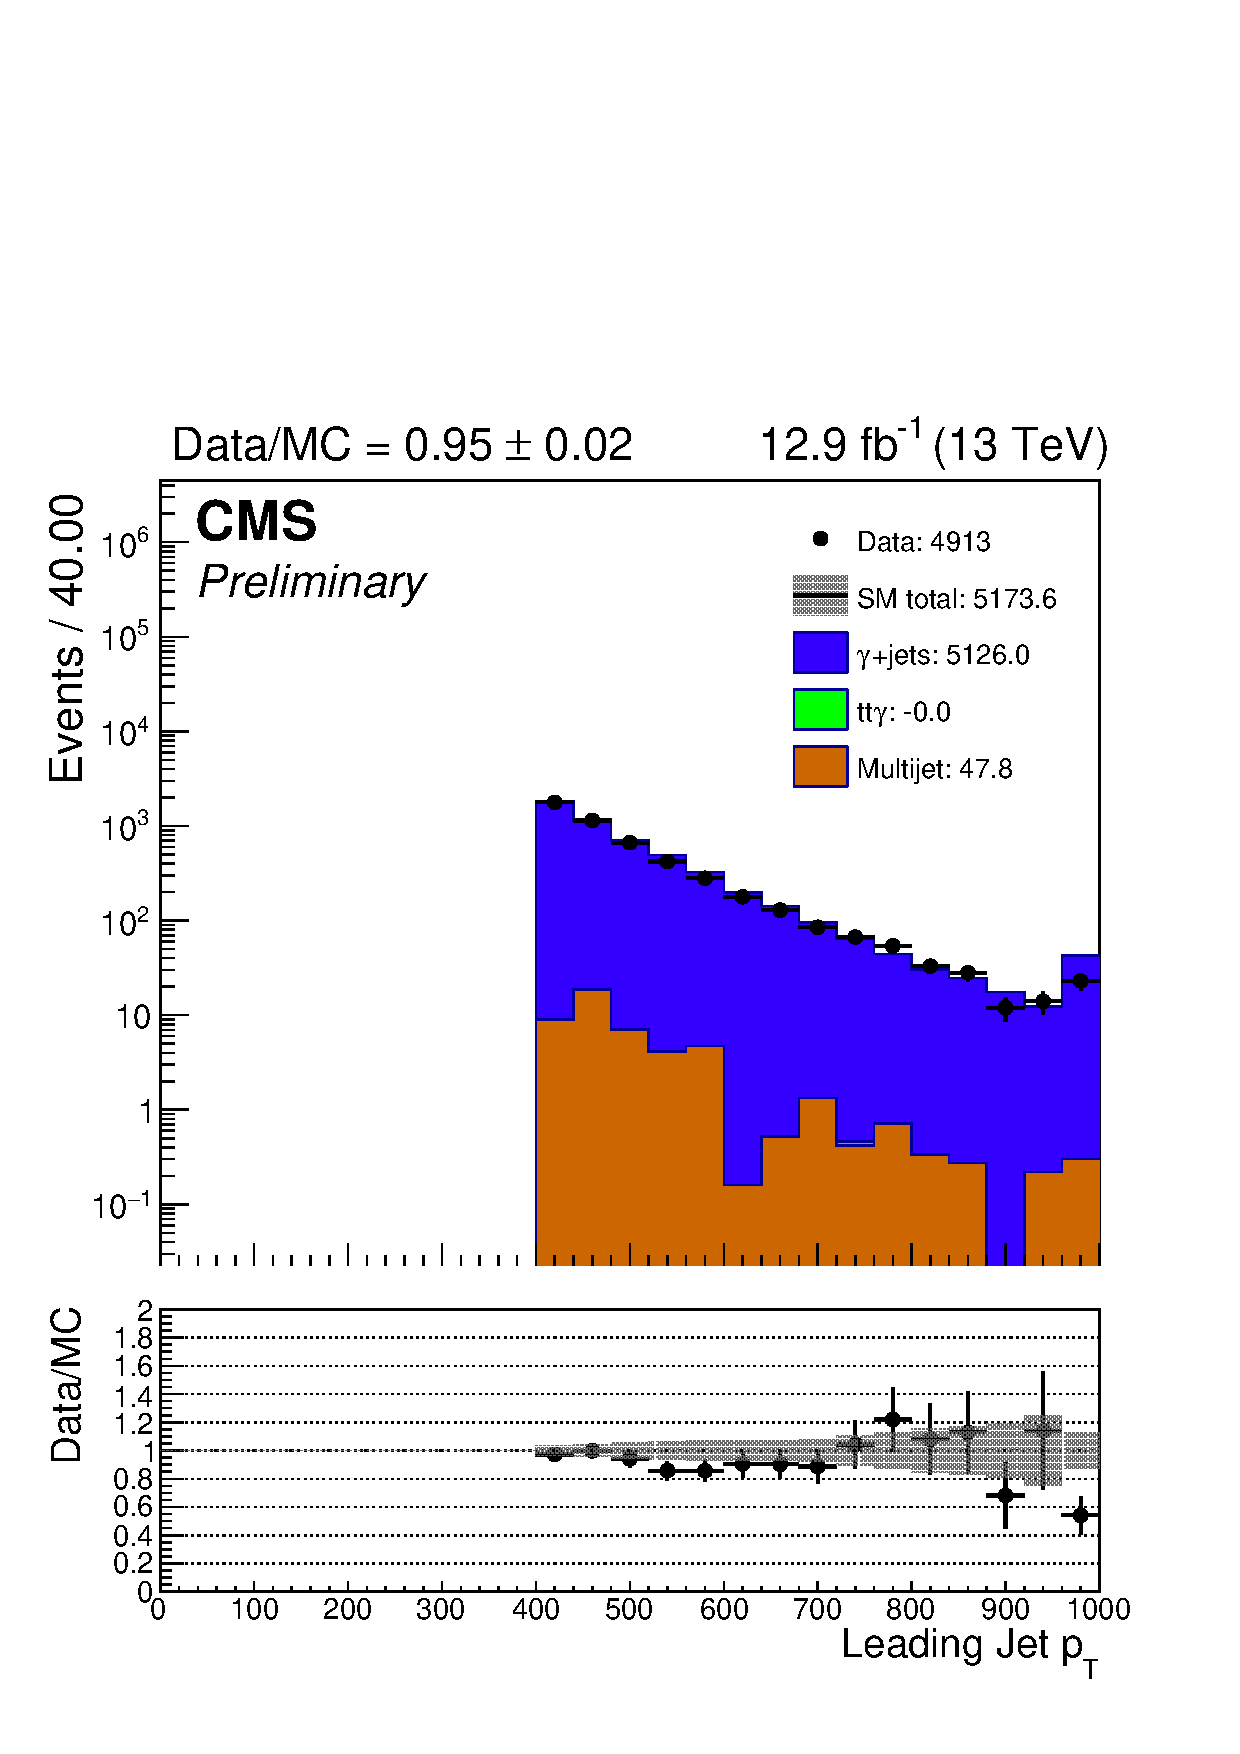
\includegraphics[width=0.5\textwidth]{figs/analysis/distributions/SinglePhoton/jet_pt[0]_eq1j.pdf}} ~~
        \subfloat {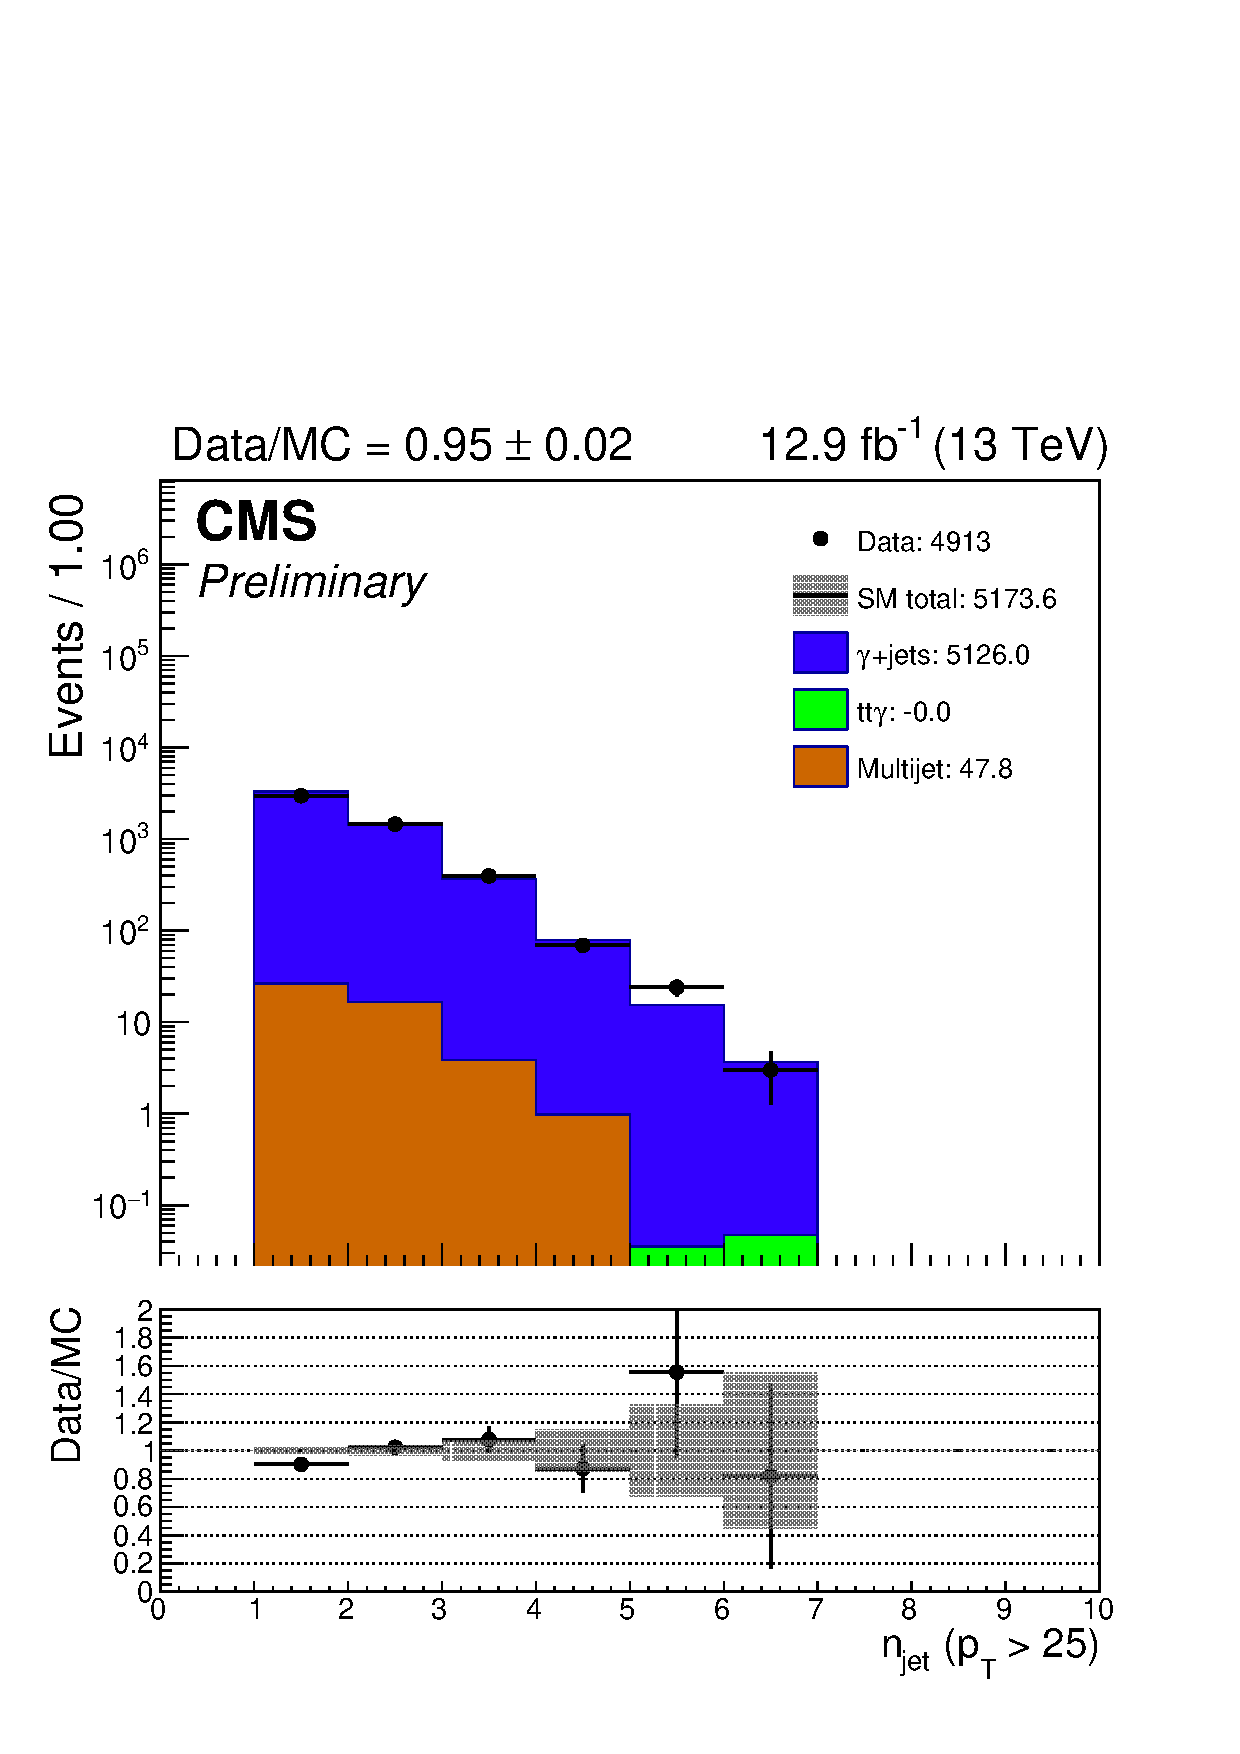
\includegraphics[width=0.5\textwidth]{figs/analysis/distributions/SinglePhoton/njetInc_eq1j.pdf}} \\
        \subfloat {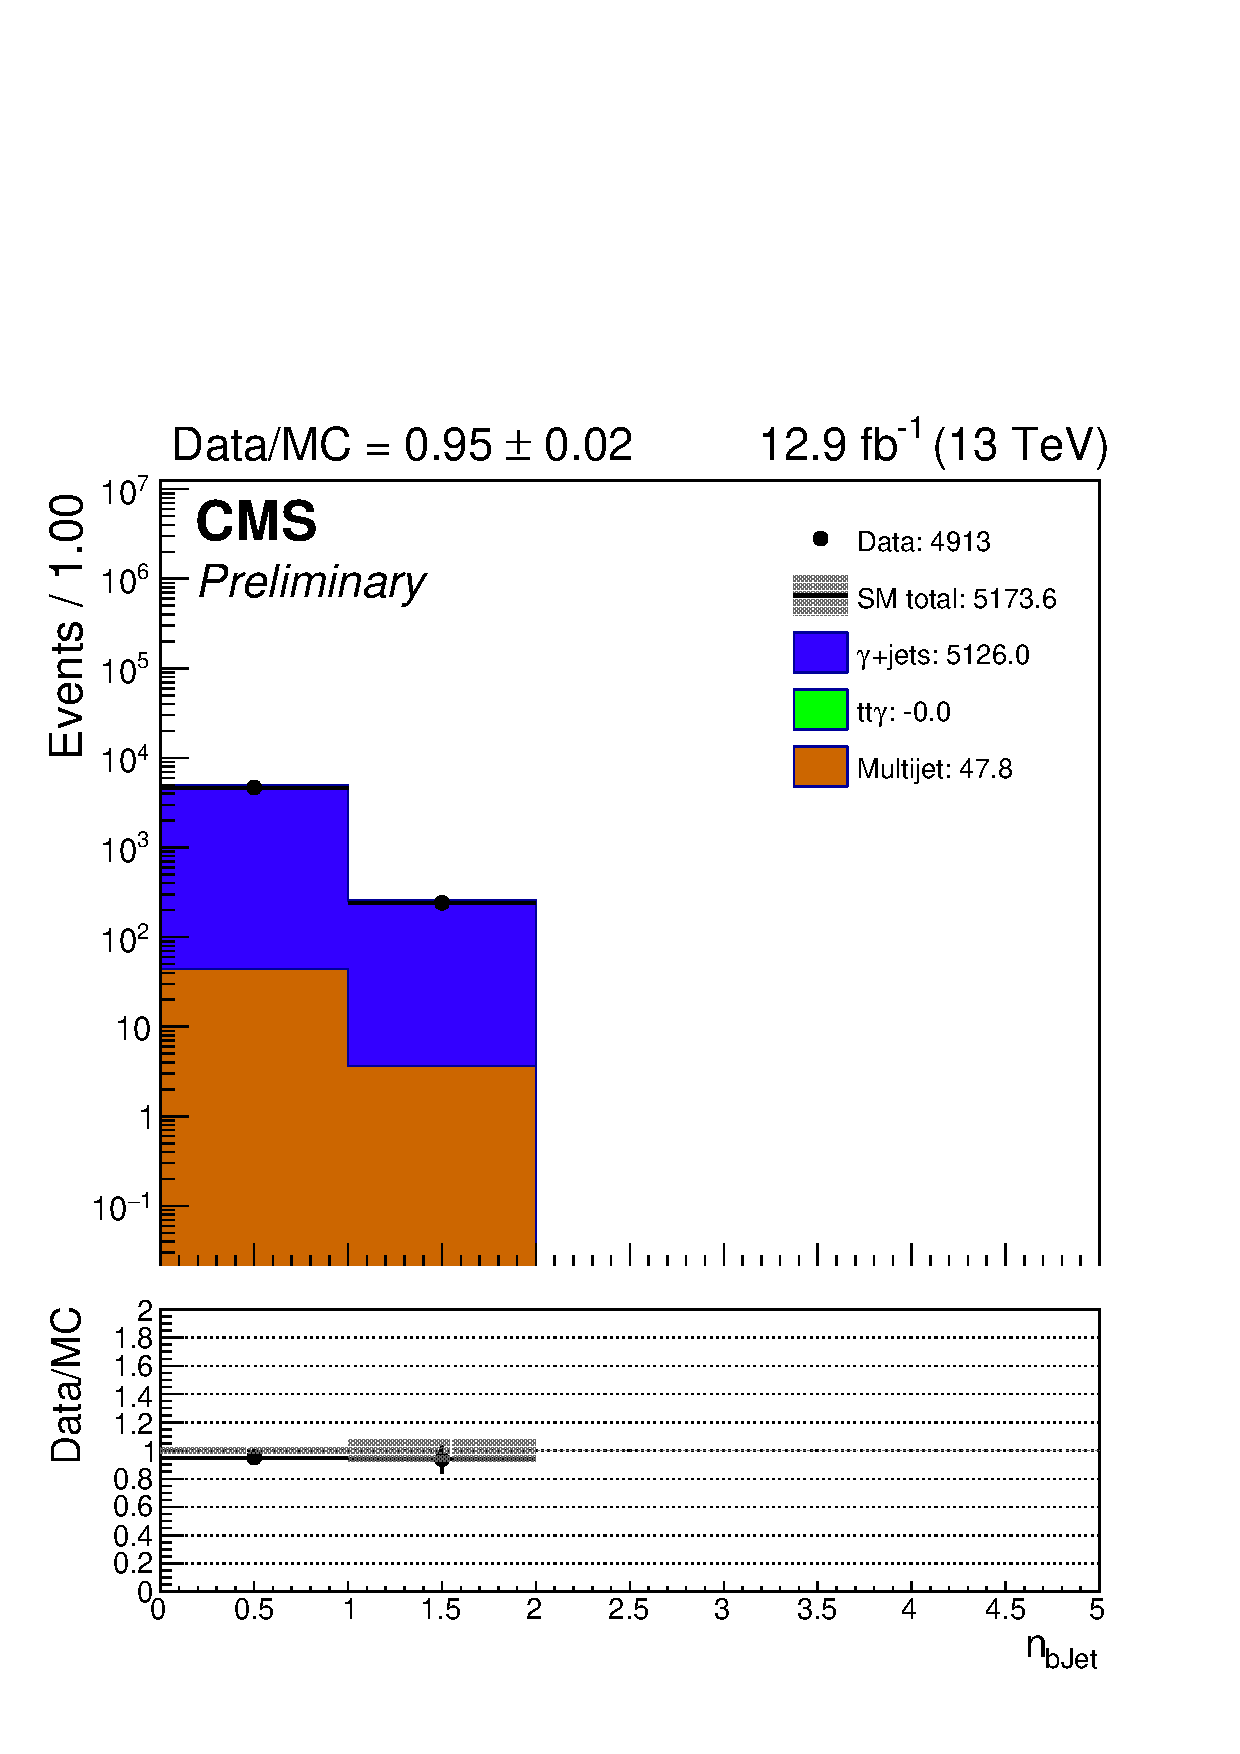
\includegraphics[width=0.5\textwidth]{figs/analysis/distributions/SinglePhoton/nBJet40_eq1j.pdf}} ~~
        \subfloat {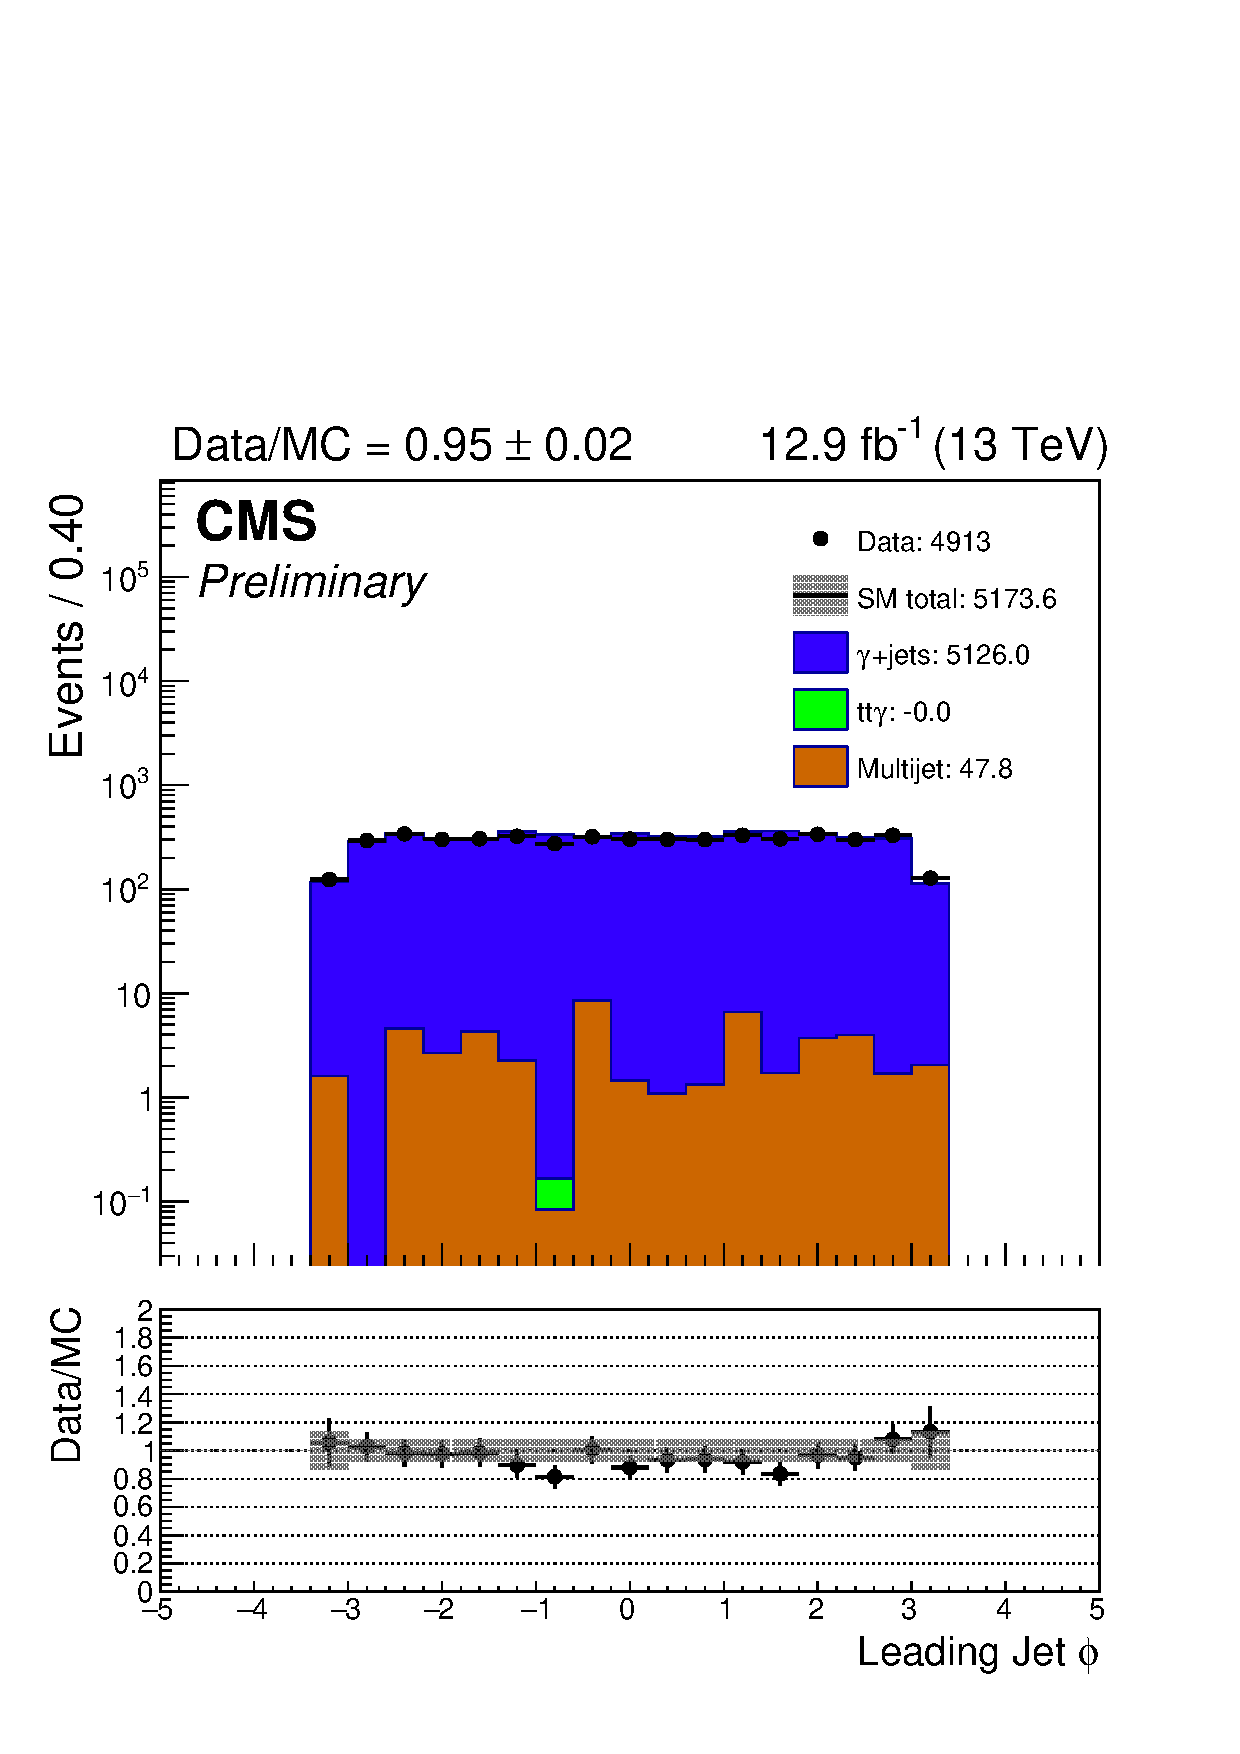
\includegraphics[width=0.5\textwidth]{figs/analysis/distributions/SinglePhoton/jet_phi[0]_eq1j.pdf}} \\
        \caption{Key analysis variables for single photon control region (monojet bins)}
        \label{fig:distribution_singlephoton_mono}
    \end{center}
\end{figure}

% \clearpage
% \subsection{Expected yields and distributions in the signal region}
\clearpage
\begin{figure}
    \begin{center}
        \subfloat {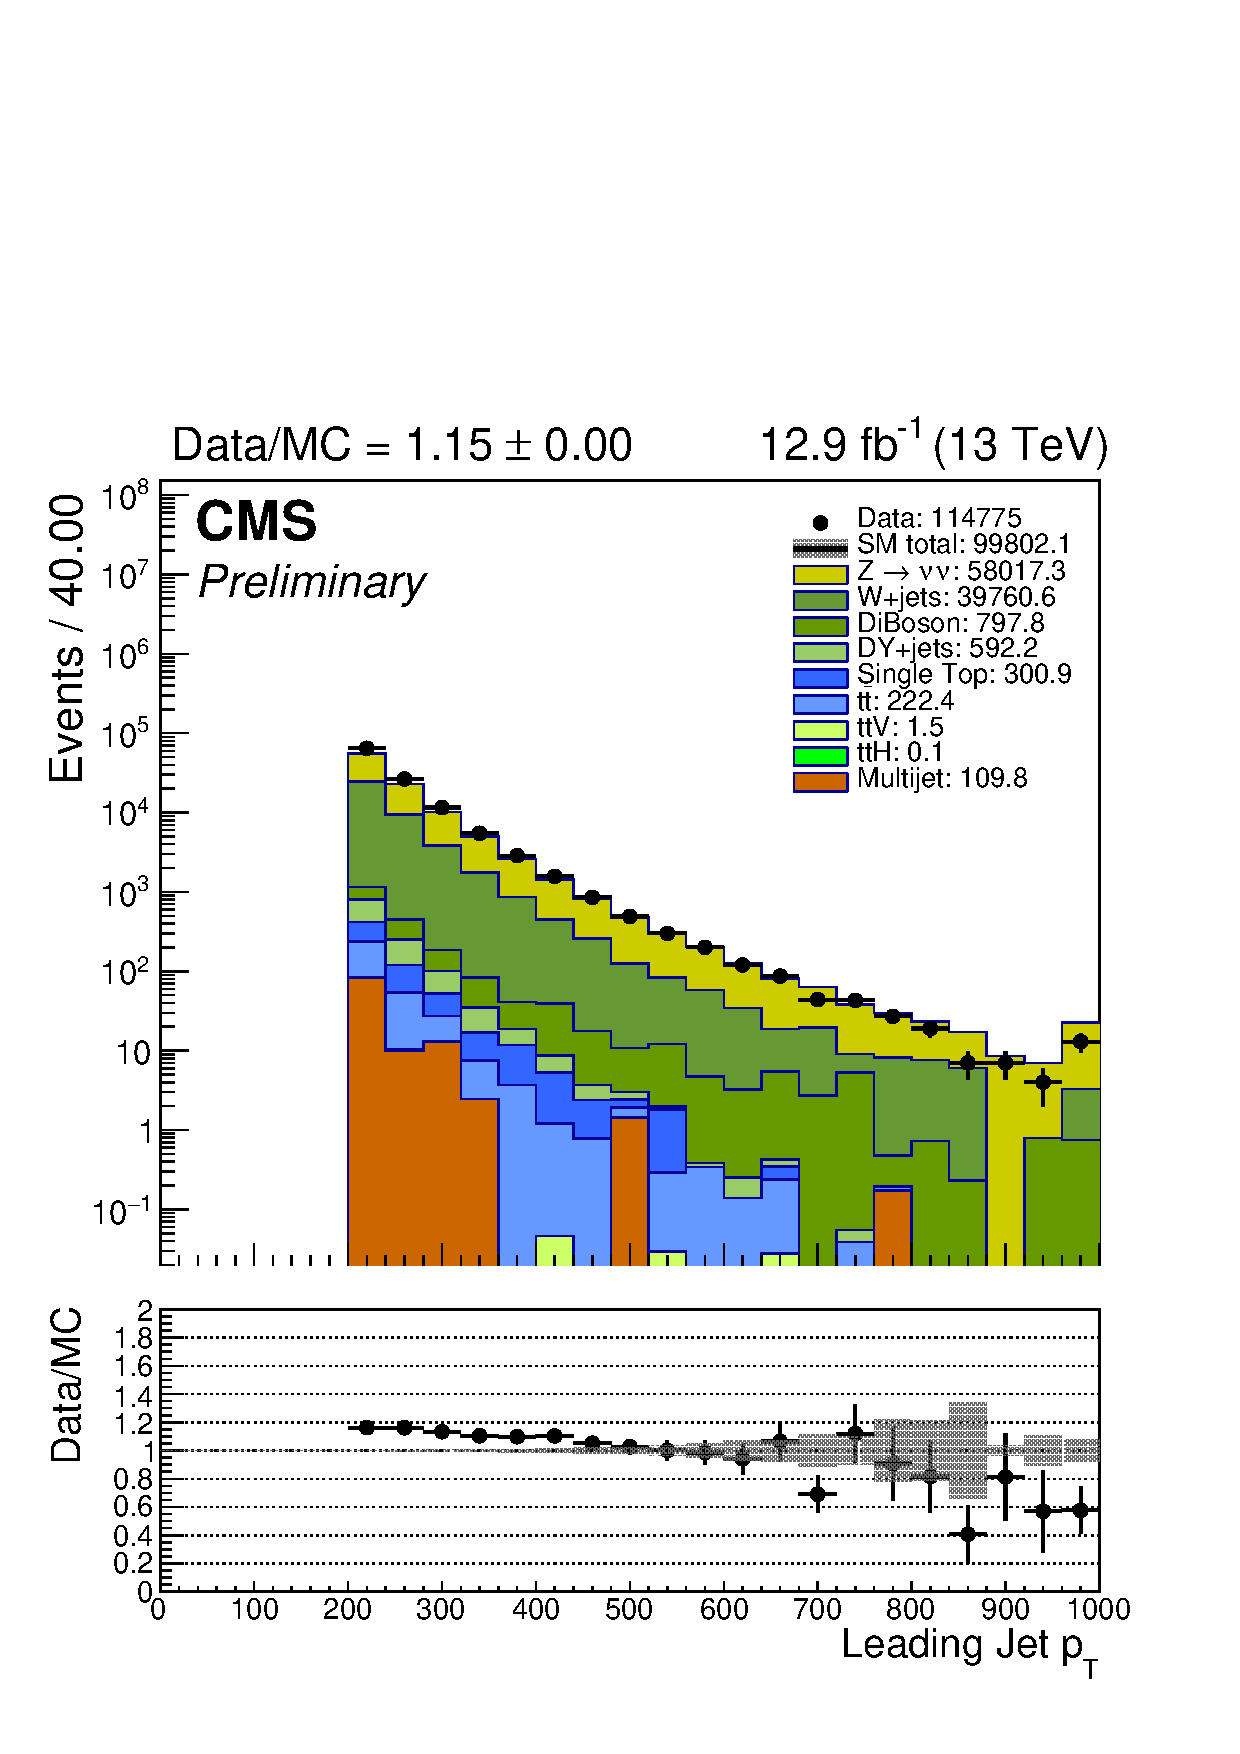
\includegraphics[width=0.5\textwidth]{figs/analysis/distributions/Signal/jet_pt[0]_eq1j.pdf}} ~~
        \subfloat {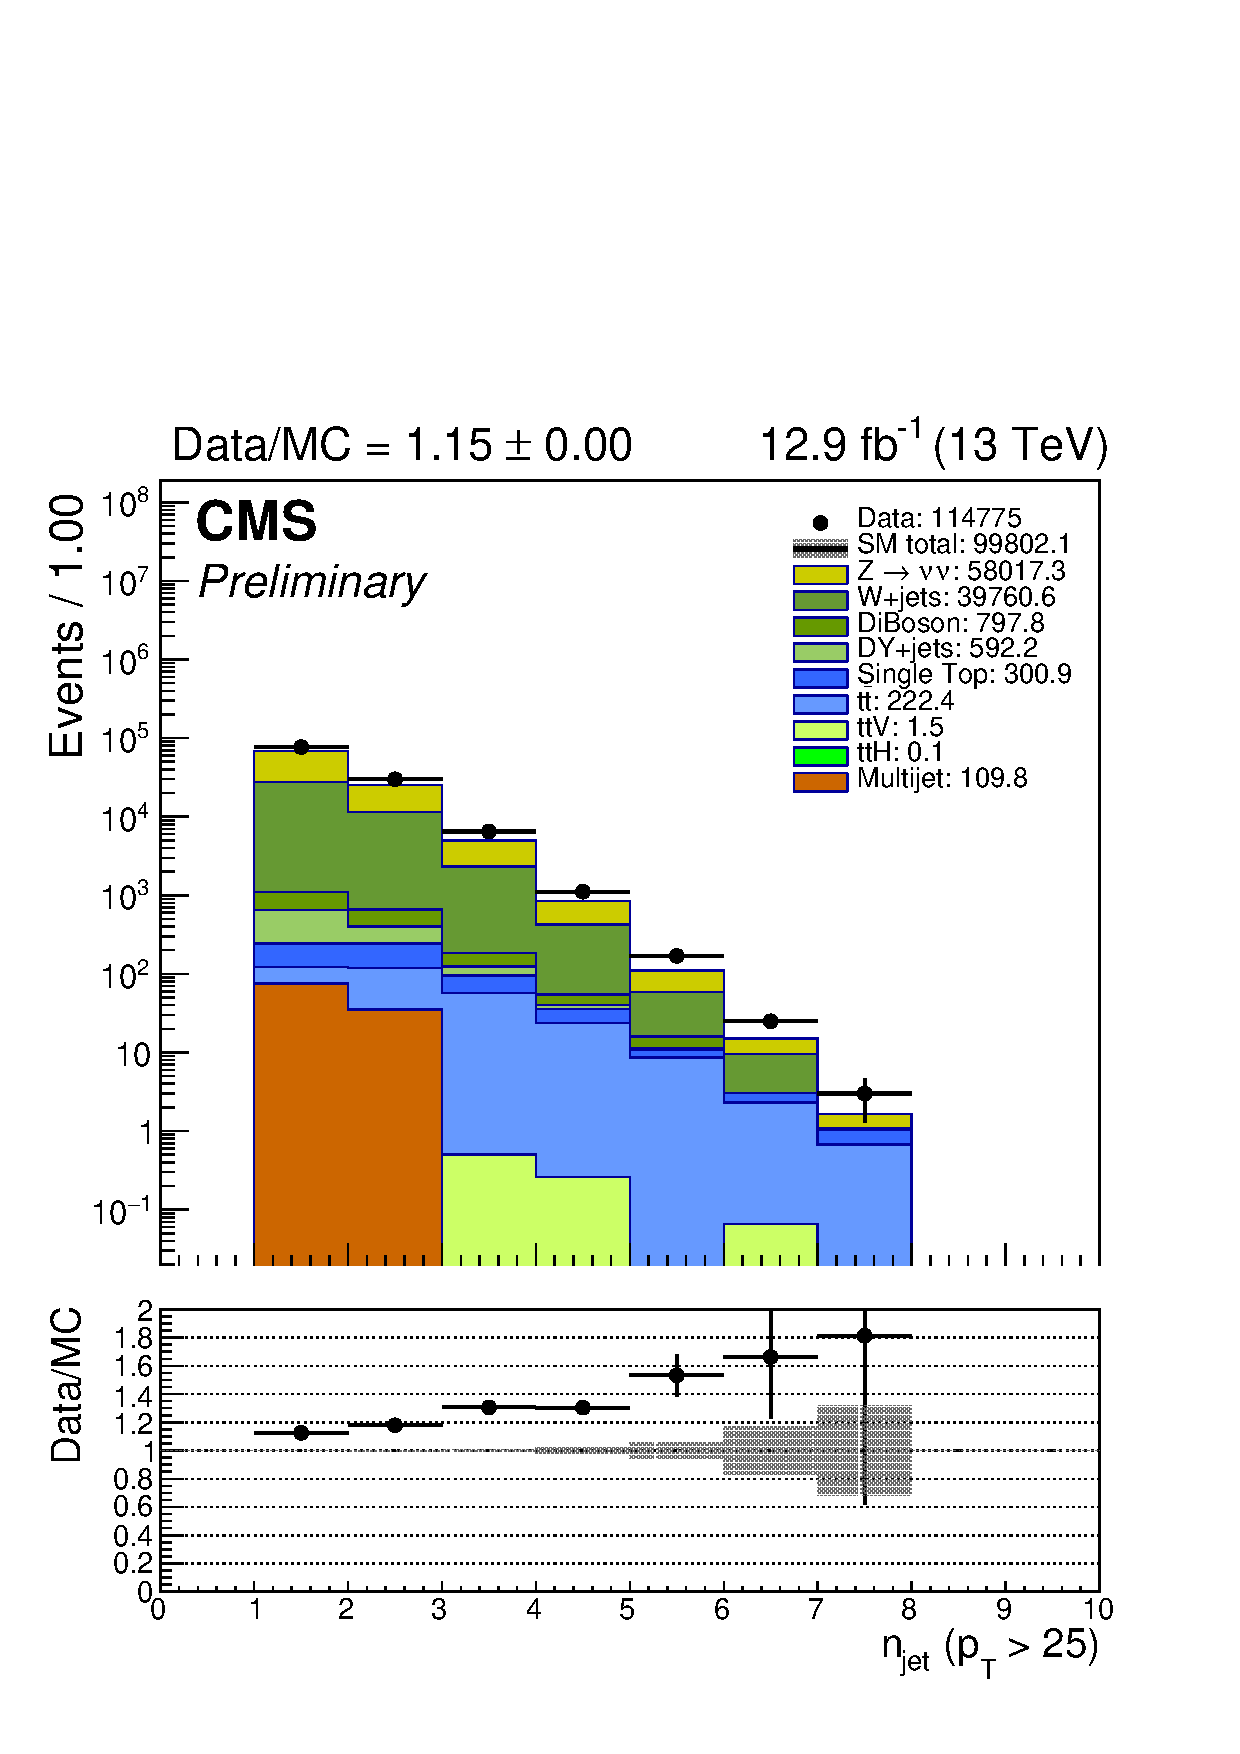
\includegraphics[width=0.5\textwidth]{figs/analysis/distributions/Signal/njetInc_eq1j.pdf}} \\
        \subfloat {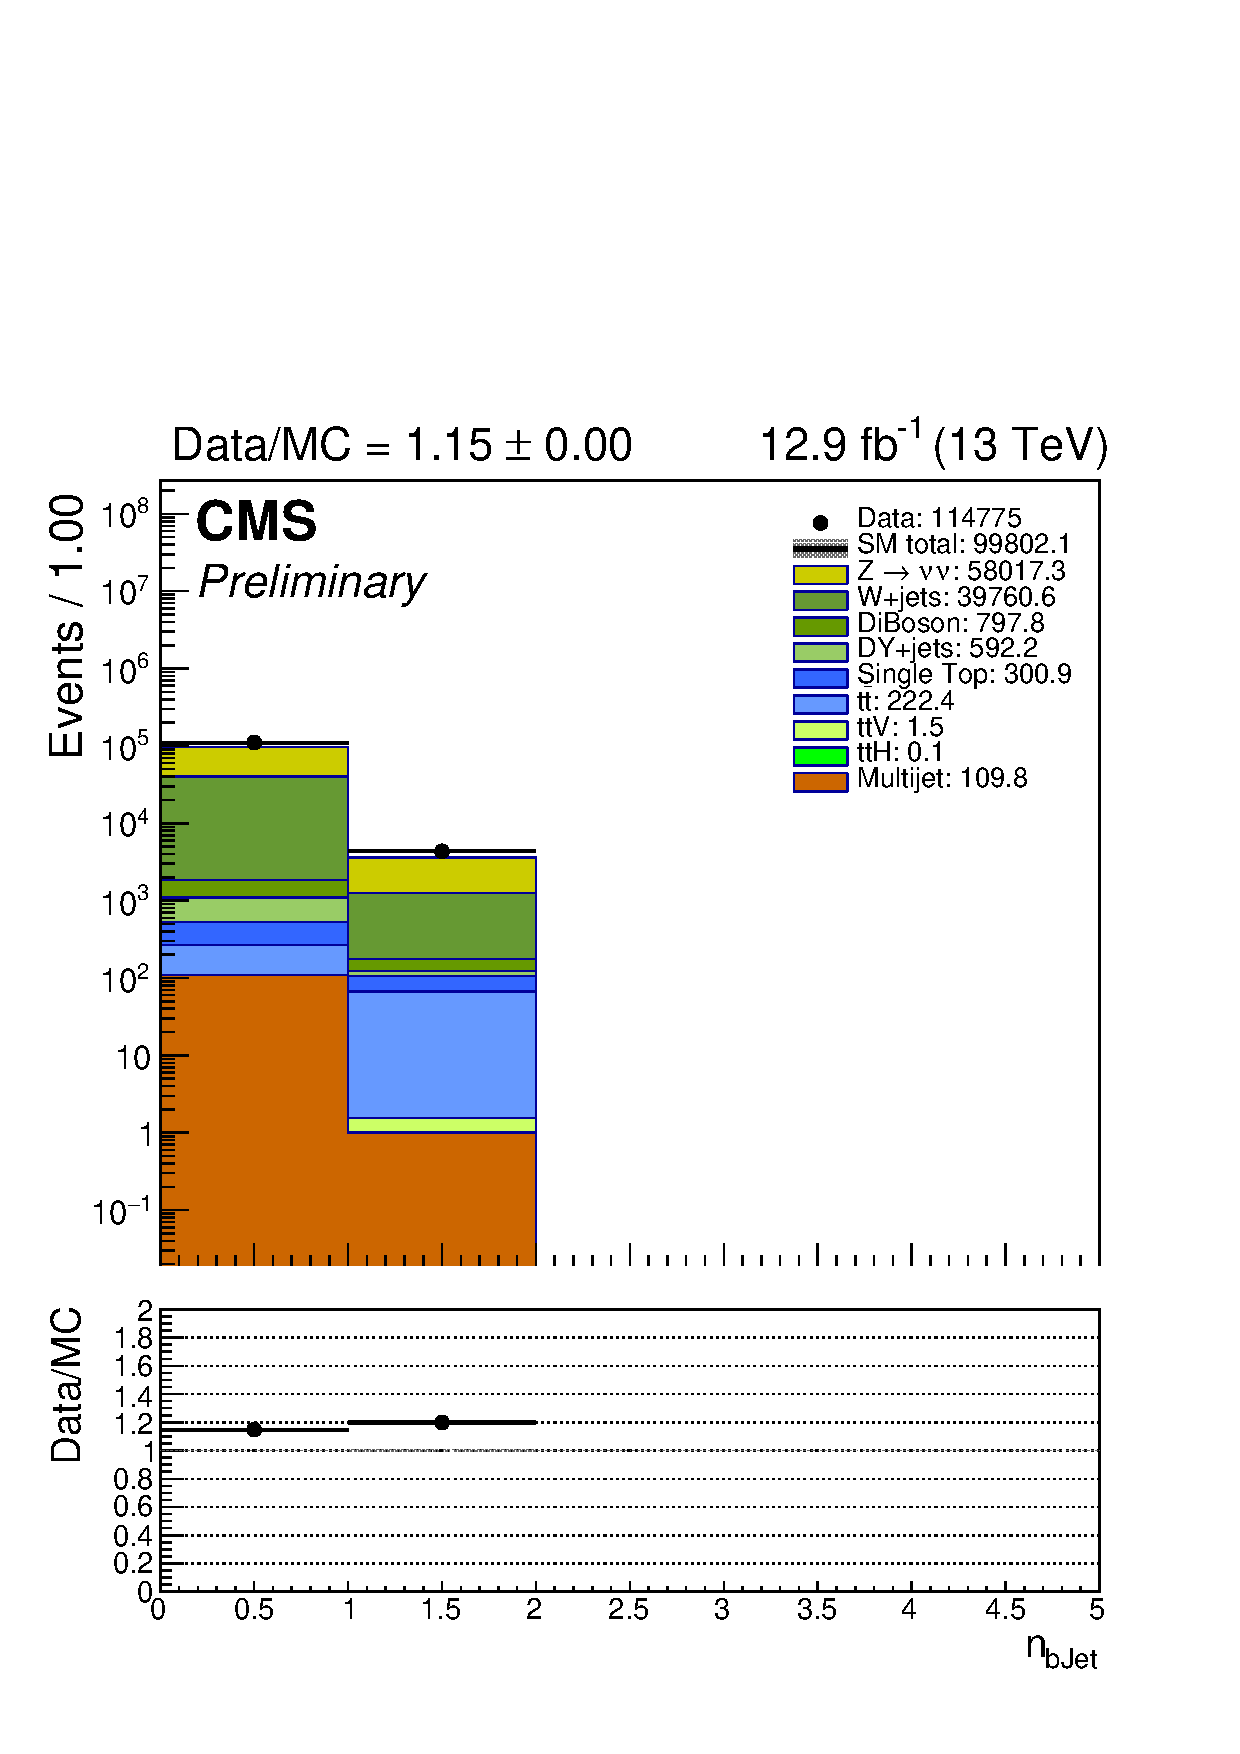
\includegraphics[width=0.5\textwidth]{figs/analysis/distributions/Signal/nBJet40_eq1j.pdf}} ~~
        \subfloat {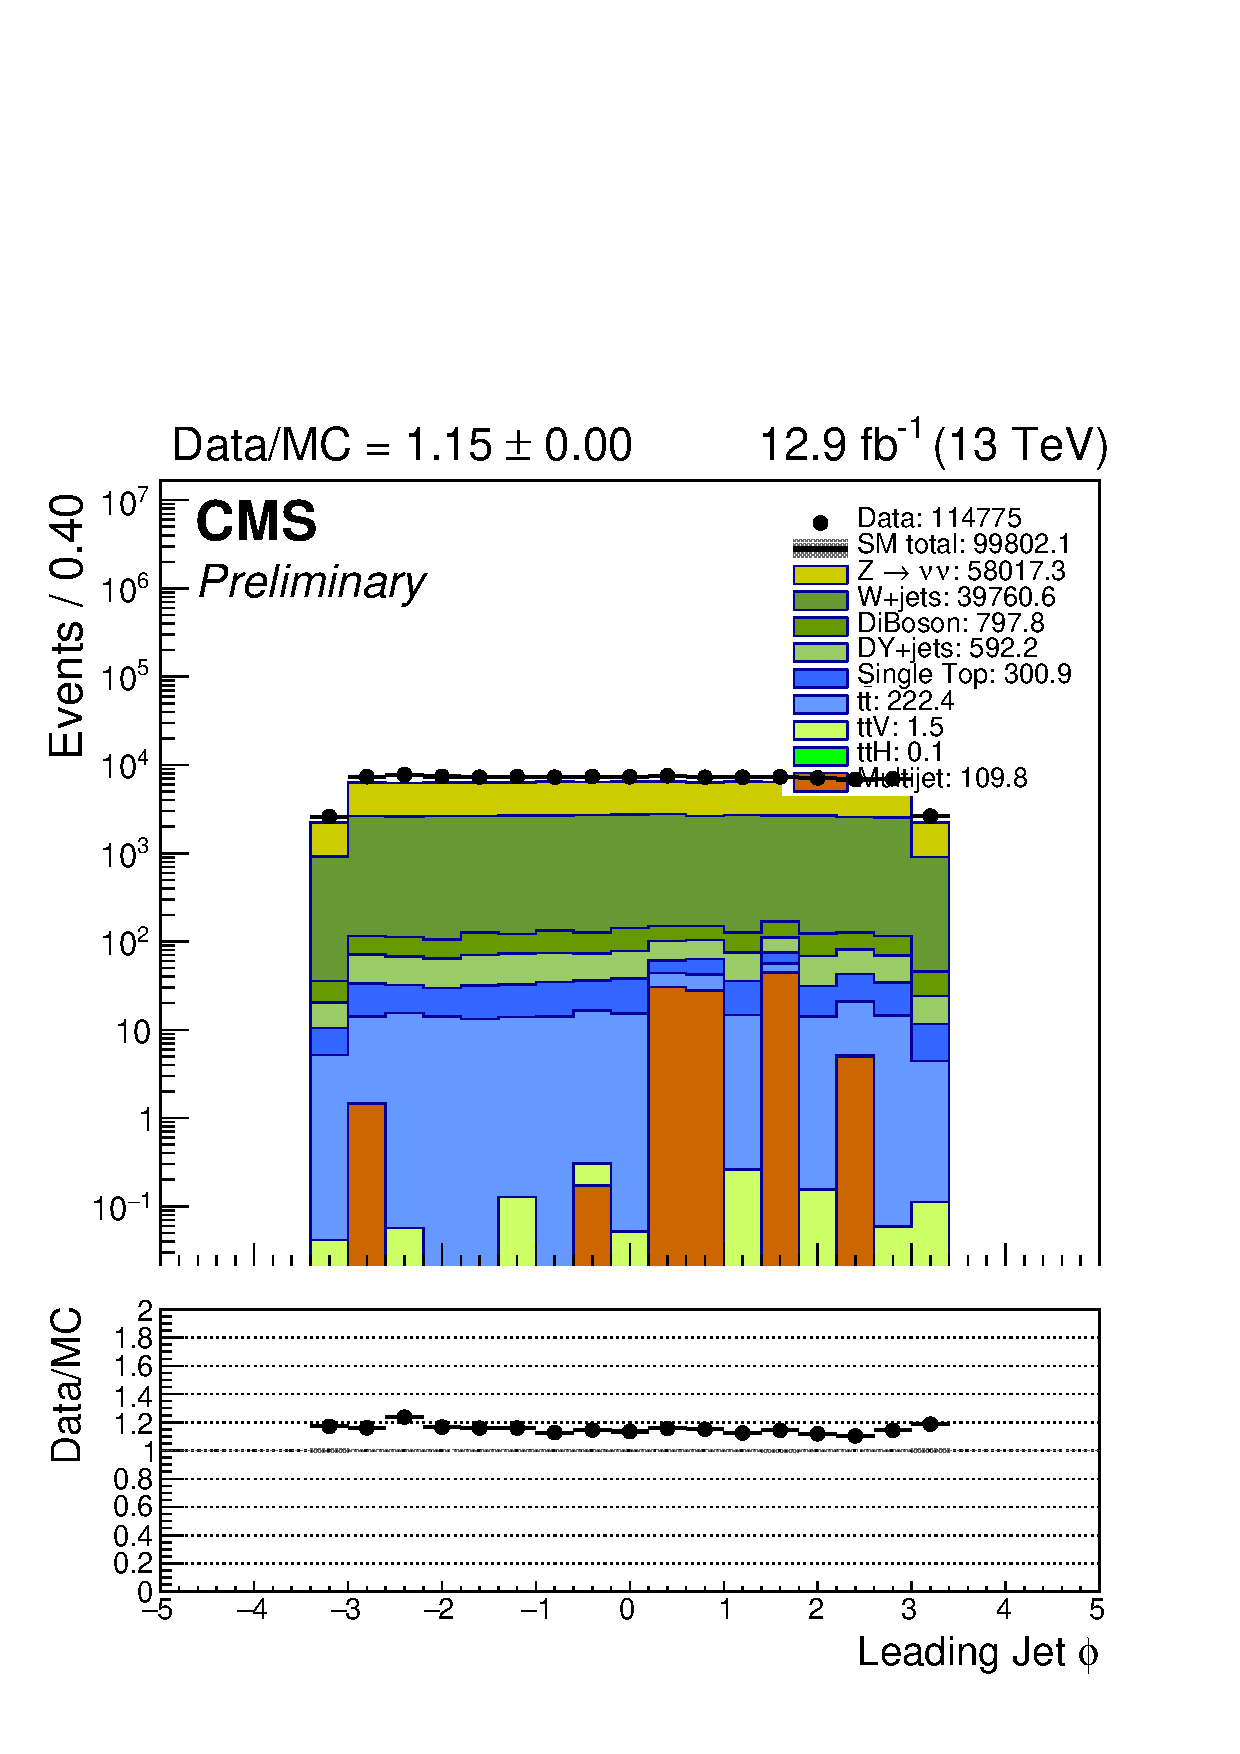
\includegraphics[width=0.5\textwidth]{figs/analysis/distributions/Signal/jet_phi[0]_eq1j.pdf}} \\
        \caption{Key analysis variables for hadronic signal region (monojet bins)}
        \label{fig:distribution_signal_mono}
    \end{center}
\end{figure}

\clearpage
\section{Binning of \MHT dimension}
\label{app:mhtBinning} 
In Tab. \ref{tab:mhtBins_eq2j}-\ref{tab:mhtBins_ge5a} the binning of
the \mht dimension for all the categories used in the analysis is
presented, for the asymmetric and symmetric topologies respectively.
Where the binning is not specified no template is used.  For the
monojet category no template is used. 

\begin{table}[h!]
  \scriptsize
  \centering
  \caption{The \mht binning for the jet category $n_{jet} = 2$. 
  \label{tab:mhtBins_eq2j}}
  \begin{tabular}{ lll }
    Jet category & $H_{T}$ bin & \mht template binning (GeV) \\ \hline

    \hline
    $\njet = 2 \;, \nb = 0 $ & $200 < H_{T} < 250$ GeV & 130, 175, 225 \\ 
     & $250 < H_{T} < 300$ GeV & 130, 175, 225, 275 \\ 
     & $300 < H_{T} < 350$ GeV & 130, 175, 225, 275, 325 \\ 
     & $350 < H_{T} < 400$ GeV & 130, 175, 225, 275, 325, 375 \\ 
     & $400 < H_{T} < 500$ GeV & 130, 175, 225, 275, 325, 375, 425, 475 \\ 
     & $500 < H_{T} < 600$ GeV & 130, 175, 225, 275, 325, 375, 425, 475, 525, 575 \\ 
     & $600 < H_{T} < 800$ GeV & 130, 175, 225, 275, 325, 375, 425, 475, 525, 575, 625, 675, 725, 775 \\ 
     & $H_{T} > 800$ GeV & 130, 250, 300, 350, 400, 450, 500, 550, 600, 650, 700, 750, 800 \\ 
    \hline
    $\njet = 2 \;, \nb = 1$ & $200 < H_{T} < 250$ GeV & 130, 175, 225 \\ 
     & $250 < H_{T} < 300$ GeV & 130, 175, 225, 275 \\ 
     & $300 < H_{T} < 350$ GeV & 130, 175, 225, 275, 325 \\ 
     & $350 < H_{T} < 400$ GeV & 130, 175, 225, 275, 325, 375 \\ 
     & $400 < H_{T} < 500$ GeV & 130, 175, 225, 275, 325, 375, 425, 475 \\ 
     & $500 < H_{T} < 600$ GeV & 130, 225, 275, 325, 375, 425, 475, 525, 575 \\ 
     & $600 < H_{T} < 800$ GeV & 130, 225, 275, 325, 375, 425, 475, 525, 575, 675, 725, 775 \\ 
     & $H_{T} > 800$ GeV & 130, 250, 300, 350, 400, 450, 500, 550, 600, 650, 700, 750, 800 \\ 
    \hline
    $\njet = 2 \;, \nb = 2 $ & $200 < H_{T} < 250$ GeV & - \\ 
     & $250 < H_{T} < 300$ GeV & 130, 175, 225, 275 \\ 
     & $300 < H_{T} < 350$ GeV & - \\ 
     & $350 < H_{T} < 400$ GeV & 130, 250, 300, 350 \\ 
     & $400 < H_{T} < 500$ GeV & - \\ 
     & $500 < H_{T} < 600$ GeV & 130, 225, 325, 375, 475, 525, 575 \\ 
     & $H_{T} > 600$ GeV & - \\ 

  \end{tabular}
\end{table}



\begin{table}[h!]
  \scriptsize
  \centering
  \caption{The \mht binning for the jet category $n_{jet} = 3$. 
  \label{tab:mhtBins_eq3j}}
  \begin{tabular}{ lll }
    Jet category & $H_{T}$ bin & \mht template binning (GeV) \\ \hline

    \hline
    $\njet = 3 \;, \nb = 0 $ & $200 < H_{T} < 250$ GeV & 130, 225 \\ 
     & $250 < H_{T} < 300$ GeV & 130, 175, 225, 275 \\ 
     & $300 < H_{T} < 350$ GeV & 130, 175, 225, 275, 325 \\ 
     & $350 < H_{T} < 400$ GeV & 130, 175, 225, 275, 325, 375 \\ 
     & $400 < H_{T} < 500$ GeV & 130, 175, 225, 275, 325, 375, 425, 475 \\ 
     & $500 < H_{T} < 600$ GeV & 130, 175, 225, 275, 325, 375, 425, 475, 525, 575 \\ 
     & $600 < H_{T} < 800$ GeV & 130, 225, 275, 325, 375, 425, 475, 525, 575, 625, 675, 725, 775 \\ 
     & $H_{T} > 800$ GeV & 130, 200, 250, 300, 350, 400, 450, 500, 550, 600, 650, 700, 750, 800 \\ 
    \hline
    $\njet = 3 \;, \nb = 1$ & $250 < H_{T} < 300$ GeV & 130, 175, 225, 275 \\ 
     & $300 < H_{T} < 350$ GeV & 130, 175, 225, 275, 325 \\ 
     & $350 < H_{T} < 400$ GeV & 130, 175, 225, 275, 325, 375 \\ 
     & $400 < H_{T} < 500$ GeV & 130, 175, 225, 275, 325, 375, 425, 475 \\ 
     & $500 < H_{T} < 600$ GeV & 130, 175, 225, 275, 325, 375, 425, 475, 525, 575 \\ 
     & $600 < H_{T} < 800$ GeV & 130, 225, 275, 325, 375, 425, 475, 525, 575, 625, 675, 725, 775 \\ 
     & $H_{T} > 800$ GeV & 130, 200, 250, 300, 350, 400, 450, 500, 550, 600, 650, 700, 750, 800 \\ 
    \hline
    $\njet = 3 \;, \nb = 2 $ & $250 < H_{T} < 300$ GeV & 130, 225, 275 \\ 
     & $300 < H_{T} < 350$ GeV & 130, 175, 225, 275, 325 \\ 
     & $350 < H_{T} < 400$ GeV & 130, 175, 225, 275, 325, 375 \\ 
     & $400 < H_{T} < 500$ GeV & 130, 175, 225, 275, 325, 375, 425 \\ 
     & $500 < H_{T} < 600$ GeV & 130, 200, 250, 300, 425, 475, 525, 575 \\ 
     & $600 < H_{T} < 800$ GeV & 130, 200, 250, 350, 400, 450, 500, 550, 600, 650, 700, 750 \\ 
     & $H_{T} > 800$ GeV & - \\ 
    \hline
    $\njet = 3 \;, \nb \geq 3$ & $250 < H_{T} < 300$ GeV & - \\ 
     & $350 < H_{T} < 400$ GeV & - \\ 
     & $H_{T} > 400$ GeV & - \\ 

  \end{tabular}
\end{table}



\begin{table}[h!]
  \scriptsize
  \centering
  \caption{The \mht binning for the jet category $n_{jet} = 4$. 
  \label{tab:mhtBins_eq4j}}
  \begin{tabular}{ lll }
    Jet category & $H_{T}$ bin & \mht template binning (GeV) \\ \hline

    \hline
    $\njet = 4 \;, \nb = 0 $ & $250 < H_{T} < 300$ GeV & - \\ 
     & $300 < H_{T} < 350$ GeV & 130, 175, 225, 275, 325 \\ 
     & $350 < H_{T} < 400$ GeV & 130, 175, 225, 275, 325, 375 \\ 
     & $400 < H_{T} < 500$ GeV & 130, 150, 200, 250, 300, 350, 400, 450 \\ 
     & $500 < H_{T} < 600$ GeV & 130, 175, 225, 275, 325, 375, 425, 475, 525, 575 \\ 
     & $600 < H_{T} < 800$ GeV & 130, 200, 250, 300, 350, 400, 450, 500, 550, 600, 650, 700, 750 \\ 
     & $H_{T} > 800$ GeV & 130, 150, 200, 250, 300, 350, 400, 450, 500, 550, 600, 650, 700, 750, 800 \\ 
    \hline
    $\njet = 4 \;, \nb = 1$ & $250 < H_{T} < 300$ GeV & - \\ 
     & $300 < H_{T} < 350$ GeV & 130, 175, 225, 275, 325 \\ 
     & $350 < H_{T} < 400$ GeV & 130, 150, 200, 250, 300, 350 \\ 
     & $400 < H_{T} < 500$ GeV & 130, 150, 200, 250, 300, 350, 400, 450 \\ 
     & $500 < H_{T} < 600$ GeV & 130, 175, 225, 275, 325, 375, 425, 475, 525 \\ 
     & $600 < H_{T} < 800$ GeV & 130, 250, 300, 350, 400, 450, 500, 550, 600, 650, 700, 750 \\ 
     & $H_{T} > 800$ GeV & 130, 150, 200, 250, 300, 350, 400, 450, 500, 550, 600, 650, 700, 750, 800 \\ 
    \hline
    $\njet = 4 \;, \nb = 2 $ & $250 < H_{T} < 300$ GeV & - \\ 
     & $300 < H_{T} < 350$ GeV & 130, 150, 200, 250, 300 \\ 
     & $350 < H_{T} < 400$ GeV & 130, 175, 225, 275, 325 \\ 
     & $400 < H_{T} < 500$ GeV & 130, 150, 200, 250, 300, 350, 400, 450 \\ 
     & $500 < H_{T} < 600$ GeV & 130, 200, 250, 300, 350, 400, 450, 500 \\ 
     & $600 < H_{T} < 800$ GeV & 130, 225, 275, 325, 375, 425, 475, 525, 575, 625, 675, 725 \\ 
     & $H_{T} > 800$ GeV & 130, 200, 250, 300, 350, 400, 450, 500, 550, 600, 650, 700, 750, 800 \\ 
    \hline
    $\njet = 4 \;, \nb \geq 3$ & $350 < H_{T} < 400$ GeV & - \\ 
     & $400 < H_{T} < 500$ GeV & - \\ 
     & $500 < H_{T} < 600$ GeV & 130, 300, 400 \\ 
     & $600 < H_{T} < 800$ GeV & - \\ 
     & $H_{T} > 800$ GeV & - \\ 

  \end{tabular}
\end{table}



\begin{table}[h!]
  \scriptsize
  \centering
  \caption{The \mht binning for the jet category $n_{jet} = 5$. 
  \label{tab:mhtBins_ge5j}}
  \begin{tabular}{ lll }
    Jet category & $H_{T}$ bin & \mht template binning (GeV) \\ \hline

    \hline
    $\njet \geq 5 \;, \nb = 0$ & $350 < H_{T} < 400$ GeV & 130, 150, 200, 250, 300, 350 \\ 
     & $400 < H_{T} < 500$ GeV & 130, 150, 200, 250, 300, 350, 400, 450 \\ 
     & $500 < H_{T} < 600$ GeV & 130, 175, 225, 275, 325, 375, 425, 475, 525 \\ 
     & $600 < H_{T} < 800$ GeV & 130, 200, 250, 300, 350, 400, 450, 500, 550, 600, 650, 700, 750 \\ 
     & $H_{T} > 800$ GeV & 130, 150, 200, 250, 300, 350, 400, 450, 500, 550, 600, 650, 700, 750, 800 \\ 
    \hline
    $\njet \geq 5 \;, \nb = 1$ & $350 < H_{T} < 400$ GeV & 130, 150, 200, 250, 300 \\ 
     & $400 < H_{T} < 500$ GeV & 130, 175, 225, 275, 325, 375, 425 \\ 
     & $500 < H_{T} < 600$ GeV & 130, 175, 225, 275, 325, 375, 425, 475, 525 \\ 
     & $600 < H_{T} < 800$ GeV & 130, 225, 275, 325, 375, 425, 475, 525, 575, 625, 675, 725 \\ 
     & $H_{T} > 800$ GeV & 130, 150, 200, 250, 300, 350, 400, 450, 500, 550, 600, 650, 700, 750, 800 \\ 
    \hline
    $\njet \geq 5 \;, \nb = 2$ & $350 < H_{T} < 400$ GeV & 130, 175, 225, 275 \\ 
     & $400 < H_{T} < 500$ GeV & 130, 150, 200, 250, 300, 350 \\ 
     & $500 < H_{T} < 600$ GeV & 130, 200, 250, 300, 350, 400, 450 \\ 
     & $600 < H_{T} < 800$ GeV & 130, 200, 250, 300, 350, 400, 450, 500, 550, 600, 650 \\ 
     & $H_{T} > 800$ GeV & 130, 150, 200, 250, 300, 350, 400, 450, 500, 550, 600, 650, 700, 750, 800 \\ 
    \hline
    $\njet \geq 5 \;, \nb \geq 3$ & $400 < H_{T} < 500$ GeV & - \\ 
     & $500 < H_{T} < 600$ GeV & - \\ 
     & $600 < H_{T} < 800$ GeV & 130, 225, 275, 325, 375, 425, 475, 525, 575 \\ 
     & $H_{T} > 800$ GeV & 130, 200, 250, 300, 350, 400, 450, 500, 550, 650, 700, 800 \\ 

  \end{tabular}
\end{table}



\begin{table}[h!]
  \scriptsize
  \centering
  \caption{The \mht binning for the jet category $n_{jet}^{asym} = 2$. 
  \label{tab:mhtBins_eq2a}}
  \begin{tabular}{ lll }
    Jet category & $H_{T}$ bin & \mht template binning (GeV) \\ \hline

    \hline
    $\njet^{\mathrm{asy}}  =   2 \;, \nb = 0 $ & $200 < H_{T} < 250$ GeV & 130, 175, 225 \\ 
     & $250 < H_{T} < 300$ GeV & 130, 225, 275 \\ 
     & $300 < H_{T} < 350$ GeV & 130, 275, 325 \\ 
     & $350 < H_{T} < 400$ GeV & 130, 325, 375 \\ 
     & $400 < H_{T} < 500$ GeV & 130, 375, 425, 475 \\ 
     & $500 < H_{T} < 600$ GeV & 130, 525, 575 \\ 
     & $H_{T} > 600$ GeV & 130, 600, 650, 700, 750, 800 \\ 
    \hline
    $\njet^{\mathrm{asy}}  =   2 \;, \nb = 1$ & $200 < H_{T} < 250$ GeV & 130, 175, 225 \\ 
     & $250 < H_{T} < 300$ GeV & 130, 225, 275 \\ 
     & $300 < H_{T} < 350$ GeV & 130, 275, 325 \\ 
     & $350 < H_{T} < 400$ GeV & 130, 375 \\ 
     & $400 < H_{T} < 500$ GeV & 130, 425, 475 \\ 
     & $H_{T} > 500$ GeV & - \\ 
    \hline
    $\njet^{\mathrm{asy}}  =   2 \;, \nb = 2$ & $200 < H_{T} < 250$ GeV & 130, 175, 225 \\ 
     & $250 < H_{T} < 300$ GeV & 130, 225, 275 \\ 
     & $300 < H_{T} < 350$ GeV & 130, 325 \\ 
     & $350 < H_{T} < 400$ GeV & - \\ 
     & $H_{T} > 400$ GeV & - \\ 

  \end{tabular}
\end{table}



\begin{table}[h!]
  \scriptsize
  \centering
  \caption{The \mht binning for the jet category $n_{jet}^{asym} = 3$. 
  \label{tab:mhtBins_eq3a}}
  \begin{tabular}{ lll }
    Jet category & $H_{T}$ bin & \mht template binning (GeV) \\ \hline

    \hline
    $\njet^{\mathrm{asy}}  =   3 \;, \nb = 0 $ & $200 < H_{T} < 250$ GeV & 130, 175, 225 \\ 
     & $250 < H_{T} < 300$ GeV & 130, 175, 225, 275 \\ 
     & $300 < H_{T} < 350$ GeV & 130, 175, 225, 275, 325 \\ 
     & $350 < H_{T} < 400$ GeV & 130, 175, 225, 275, 325, 375 \\ 
     & $400 < H_{T} < 500$ GeV & 130, 225, 275, 325, 375, 425, 475 \\ 
     & $500 < H_{T} < 600$ GeV & 130, 425, 475, 525, 575 \\ 
     & $H_{T} > 600$ GeV & 130, 550, 600, 650, 700, 750, 800 \\ 
    \hline
    $\njet^{\mathrm{asy}}  =   3 \;, \nb = 1$ & $200 < H_{T} < 250$ GeV & 130, 175, 225 \\ 
     & $250 < H_{T} < 300$ GeV & 130, 175, 225, 275 \\ 
     & $300 < H_{T} < 350$ GeV & 130, 175, 225, 275, 325 \\ 
     & $350 < H_{T} < 400$ GeV & 130, 175, 225, 275, 325, 375 \\ 
     & $400 < H_{T} < 500$ GeV & 130, 225, 275, 325, 375, 425, 475 \\ 
     & $500 < H_{T} < 600$ GeV & 130, 450, 500, 550 \\ 
     & $H_{T} > 600$ GeV & 130, 550, 600, 650, 700, 750, 800 \\ 
    \hline
    $\njet^{\mathrm{asy}}  =   3 \;, \nb = 2$ & $200 < H_{T} < 250$ GeV & 130, 175, 225 \\ 
     & $250 < H_{T} < 300$ GeV & 130, 175, 225, 275 \\ 
     & $300 < H_{T} < 350$ GeV & 130, 175, 225, 275, 325 \\ 
     & $350 < H_{T} < 400$ GeV & 130, 250, 300, 350 \\ 
     & $400 < H_{T} < 500$ GeV & 130, 275, 325, 375, 425 \\ 
     & $H_{T} > 500$ GeV & 130, 575, 650, 700, 750, 800 \\ 
    \hline
    $\njet^{\mathrm{asy}}  =   3 \;, \nb \geq 3$ & $200 < H_{T} < 250$ GeV & - \\ 
     & $250 < H_{T} < 300$ GeV & - \\ 
     & $H_{T} > 300$ GeV & - \\ 

  \end{tabular}
\end{table}



\begin{table}[h!]
  \scriptsize
  \centering
  \caption{The \mht binning for the jet category $n_{jet}^{asym} = 4$. 
  \label{tab:mhtBins_eq4a}}
  \begin{tabular}{ lll }
    Jet category & $H_{T}$ bin & \mht template binning (GeV) \\ \hline

    \hline
    $\njet^{\mathrm{asy}}  =   4 \;, \nb = 0 $ & $200 < H_{T} < 250$ GeV & 130, 175, 225 \\ 
     & $250 < H_{T} < 300$ GeV & 130, 175, 225, 275 \\ 
     & $300 < H_{T} < 350$ GeV & 130, 175, 225, 275, 325 \\ 
     & $350 < H_{T} < 400$ GeV & 130, 175, 225, 275, 325, 375 \\ 
     & $400 < H_{T} < 500$ GeV & 130, 150, 200, 250, 300, 350, 400, 450 \\ 
     & $500 < H_{T} < 600$ GeV & 130, 250, 300, 350, 400, 450, 500, 550 \\ 
     & $H_{T} > 600$ GeV & 130, 450, 500, 550, 600, 650, 700, 750, 800 \\ 
    \hline
    $\njet^{\mathrm{asy}}  =   4 \;, \nb = 1$ & $200 < H_{T} < 250$ GeV & - \\ 
     & $250 < H_{T} < 300$ GeV & 130, 175, 225, 275 \\ 
     & $300 < H_{T} < 350$ GeV & 130, 175, 225, 275, 325 \\ 
     & $350 < H_{T} < 400$ GeV & 130, 150, 200, 250, 300, 350 \\ 
     & $400 < H_{T} < 500$ GeV & 130, 150, 200, 250, 300, 350, 400, 450 \\ 
     & $500 < H_{T} < 600$ GeV & 130, 250, 300, 350, 400, 450, 500, 550 \\ 
     & $H_{T} > 600$ GeV & 130, 500, 550, 600, 650, 700, 750, 800 \\ 
    \hline
    $\njet^{\mathrm{asy}}  =   4 \;, \nb = 2$ & $200 < H_{T} < 250$ GeV & - \\ 
     & $250 < H_{T} < 300$ GeV & 130, 175, 225, 275 \\ 
     & $300 < H_{T} < 350$ GeV & 130, 150, 200, 250, 300 \\ 
     & $350 < H_{T} < 400$ GeV & 130, 175, 225, 275, 325 \\ 
     & $400 < H_{T} < 500$ GeV & 130, 150, 200, 250, 300, 350, 400 \\ 
     & $500 < H_{T} < 600$ GeV & 130, 325, 375, 425, 475, 525 \\ 
     & $H_{T} > 600$ GeV & - \\ 
    \hline
    $\njet^{\mathrm{asy}}  =   4 \;, \nb \geq 3$ & $250 < H_{T} < 300$ GeV & - \\ 
     & $300 < H_{T} < 350$ GeV & - \\ 
     & $350 < H_{T} < 400$ GeV & 130, 175, 225, 275 \\ 
     & $H_{T} > 400$ GeV & - \\ 

  \end{tabular}
\end{table}



\begin{table}[h!]
  \scriptsize
  \centering
  \caption{The \mht binning for the jet category $n_{jet}^{asym} = 5$. 
  \label{tab:mhtBins_ge5a}}
  \begin{tabular}{ lll }
    Jet category & $H_{T}$ bin & \mht template binning (GeV) \\ \hline

    \hline
    $\njet^{\mathrm{asy}} \geq 5 \;, \nb = 0 $ & $250 < H_{T} < 300$ GeV & - \\ 
     & $300 < H_{T} < 350$ GeV & 130, 150, 200, 250, 300 \\ 
     & $350 < H_{T} < 400$ GeV & 130, 150, 200, 250, 300, 350 \\ 
     & $400 < H_{T} < 500$ GeV & 130, 175, 225, 275, 325, 375, 425 \\ 
     & $500 < H_{T} < 600$ GeV & 130, 200, 250, 300, 350, 400, 450, 500, 550 \\ 
     & $H_{T} > 600$ GeV & 130, 250, 300, 350, 400, 450, 500, 550, 600, 650, 700, 750, 800 \\ 
    \hline
    $\njet^{\mathrm{asy}} \geq 5 \;, \nb = 1$ & $250 < H_{T} < 300$ GeV & - \\ 
     & $300 < H_{T} < 350$ GeV & 130, 150, 200, 250, 300 \\ 
     & $350 < H_{T} < 400$ GeV & 130, 175, 225, 275, 325 \\ 
     & $400 < H_{T} < 500$ GeV & 130, 150, 200, 250, 300, 350, 400 \\ 
     & $500 < H_{T} < 600$ GeV & 130, 175, 225, 275, 325, 375, 425, 500 \\ 
     & $H_{T} > 600$ GeV & 130, 225, 275, 325, 375, 450, 500, 550, 600, 650, 700, 750, 800 \\ 
    \hline
    $\njet^{\mathrm{asy}} \geq 5 \;, \nb = 2$ & $250 < H_{T} < 300$ GeV & - \\ 
     & $300 < H_{T} < 350$ GeV & 130, 150, 200, 250 \\ 
     & $350 < H_{T} < 400$ GeV & 130, 150, 200, 250, 300 \\ 
     & $400 < H_{T} < 500$ GeV & 130, 150, 200, 250, 300, 350 \\ 
     & $500 < H_{T} < 600$ GeV & 130, 175, 225, 275, 325, 375, 425 \\ 
     & $H_{T} > 600$ GeV & 130, 275, 325, 375, 450, 500, 600, 700 \\ 
    \hline
    $\njet^{\mathrm{asy}} \geq 5 \;, \nb \geq 3$ & $300 < H_{T} < 350$ GeV & - \\ 
     & $350 < H_{T} < 400$ GeV & 130, 150, 200, 250 \\ 
     & $400 < H_{T} < 500$ GeV & - \\ 
     & $H_{T} > 500$ GeV & - \\ 

  \end{tabular}
\end{table}

\clearpage
\section{Bin labels key}
\label{app:plotKey}

The \nj ~categories are labelled with four letter strings that indicate
the number of jets and the topology, $a$ for asymmetric and $j$ for
symmetric. The \nb categories contain the letter $b$. The number of
jets is represented by the number and is prefixed by either \emph{eq}
corresponding to $=$, or \emph{ge} corresponding to $\geq$.

The \HT bins are labelled based on their lower bin edge in \gev. This
bin extends up to the next \HT bin, with the exception of $800$ which
is open ended.

As an example, \emph{HT250 eq4j} would correspond to the
$250<\HT<300~\gev$ bin with $\nj=4$ and a symmetric topology.
Alternatively, \emph{HT800 ge5a} would correspond to the
$800<\HT<\inf~\gev$ bin with $\nj\geq5$ and an asymmetric topology.

\section{Variation in transfer factors from known systematic
uncertainties}
\label{app:tfSysts}

The variations of the transfer factors after variations of known
sources of systematic uncertainty, as discussed in
Sec.~\ref{sec:simUnc}. These are shown for all relevant transfer
factors from the \gj,\mj and \mmj control samples. The plots are
labelled as described in the key in Appendix~\ref{app:plotKey}.

\begin{figure}[!h]
  \centering
  \subfloat[b-tag SF (heavy) up variation]{
    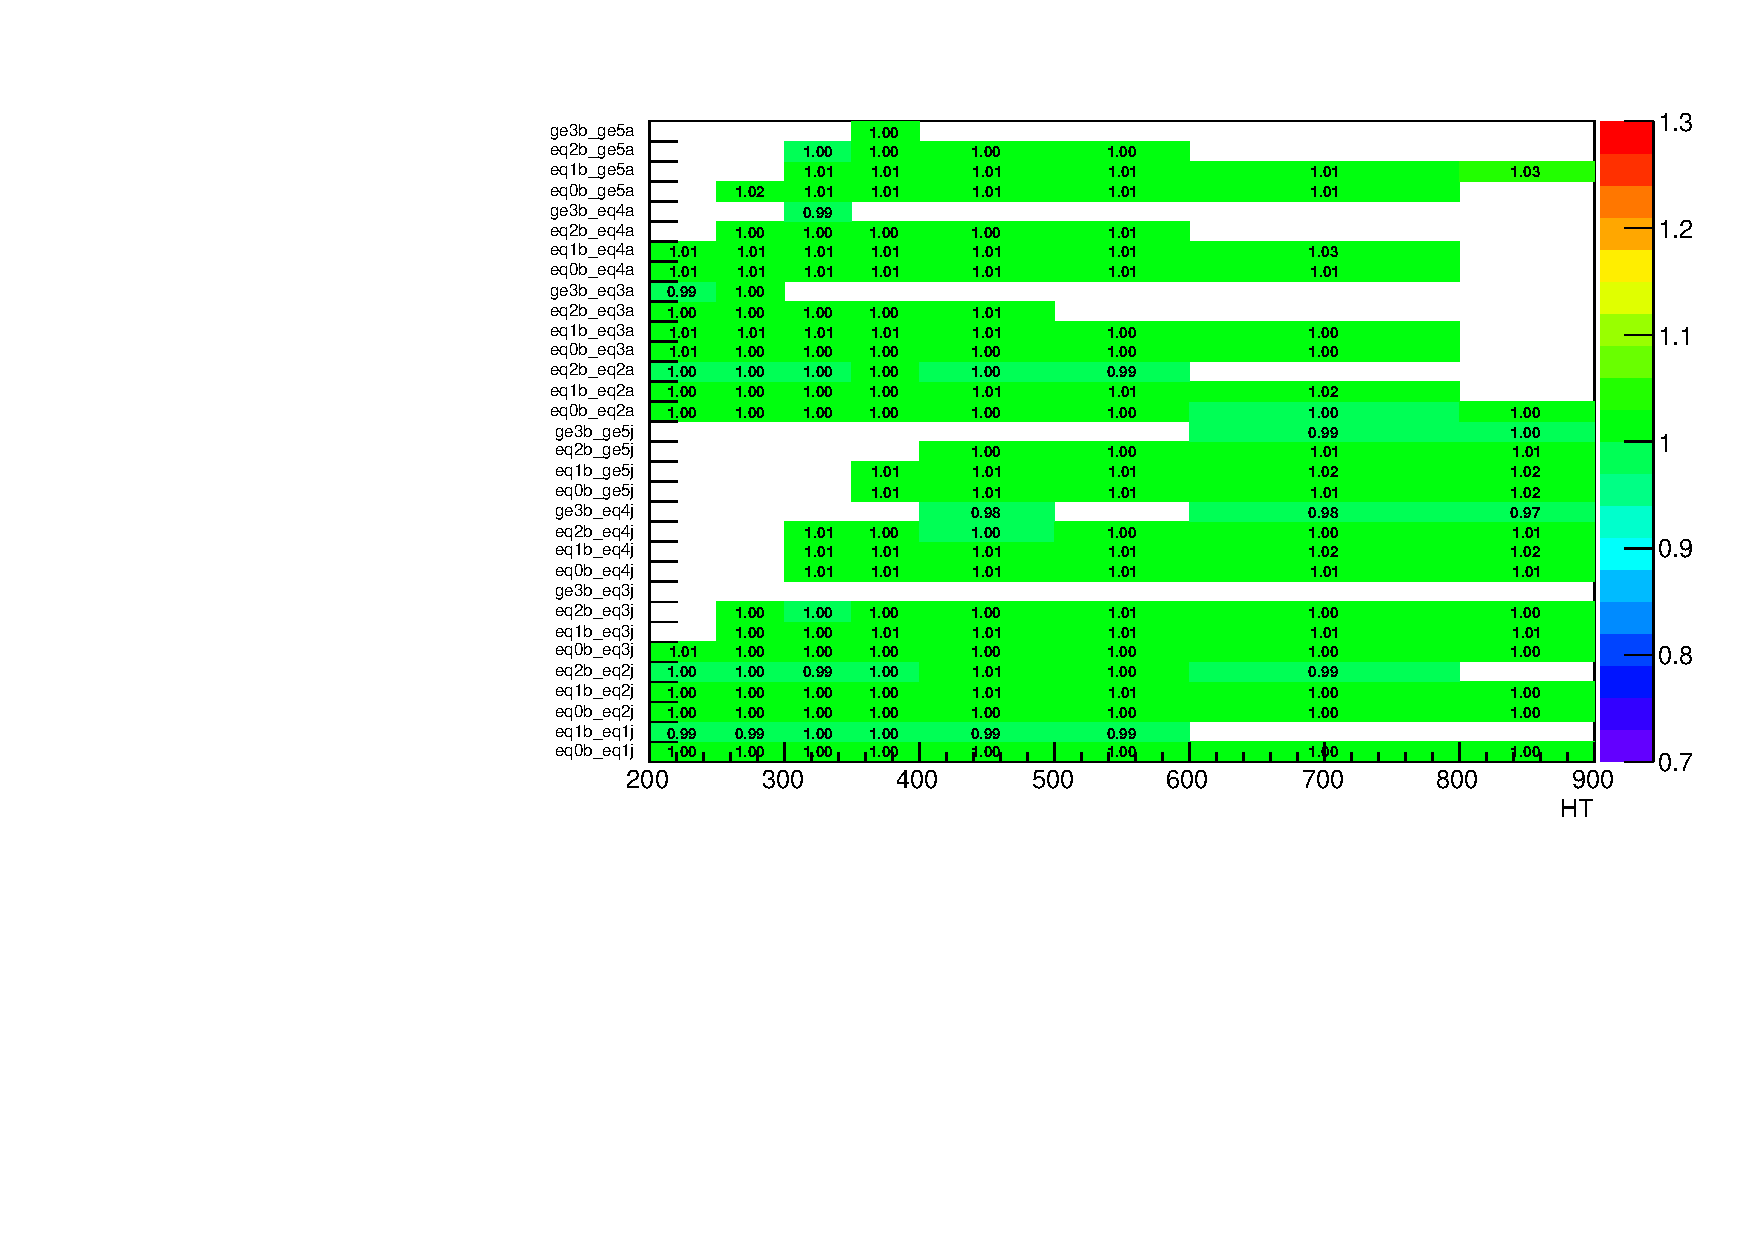
\includegraphics[width=0.5\textwidth]{figs/analysis/systsTf/Zinv/mu/ratiotfh_ht_mht_allbsfWeight_Up.pdf}
  } ~~
  \subfloat[b-tag SF (heavy) down variation]{
    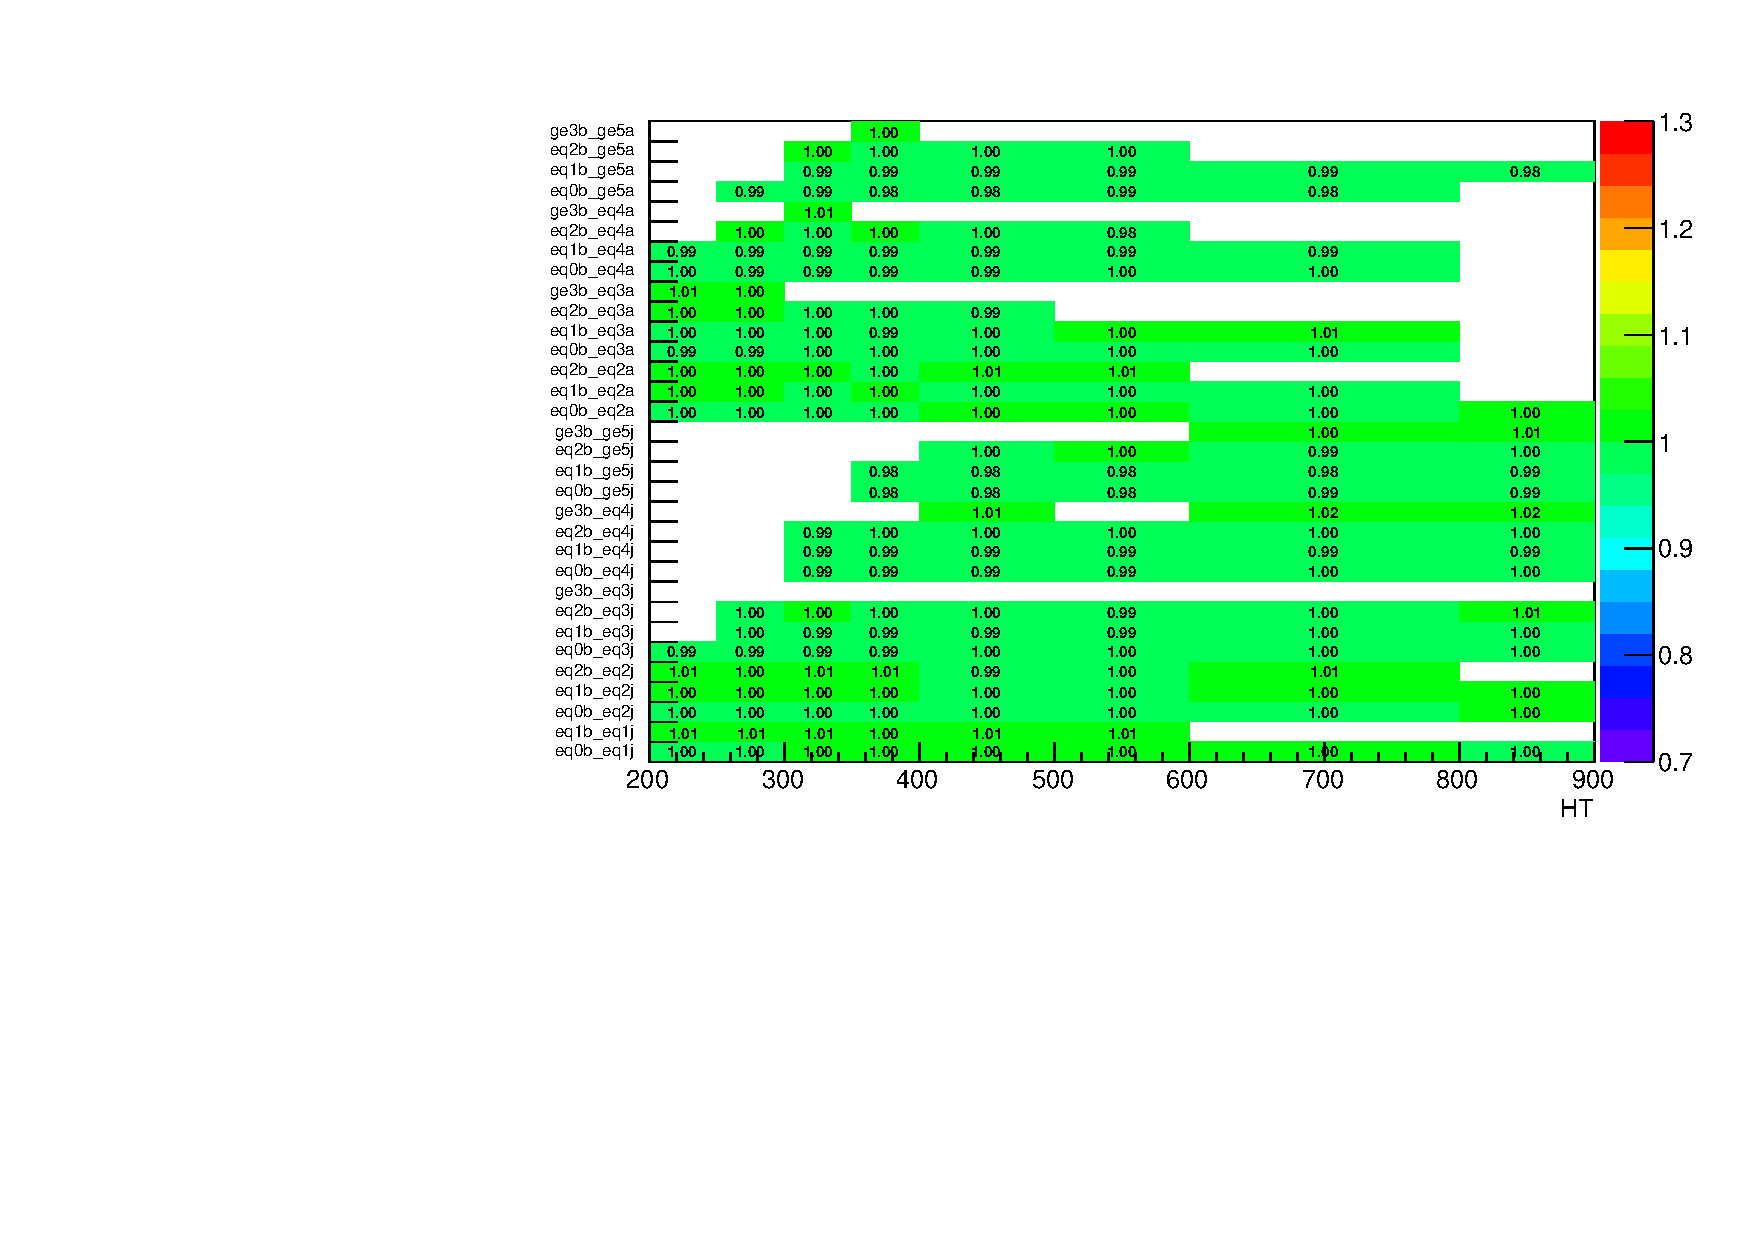
\includegraphics[width=0.5\textwidth]{figs/analysis/systsTf/Zinv/mu/ratiotfh_ht_mht_allbsfWeight_Down.pdf}
  }\\

  \caption{\label{fig:tfSyst_bsf_muToZinv} The relative change in the
  $\mj \rightarrow (\znunu)$ transfer
  factors when varying b-tag SF for heavy jets in MC within its uncertainties, as a function of \scalht and jet category. 
  Variations corresponding to $+1\sigma$ ($-1\sigma$) are shown in the left (right) figure. 
  }
\end{figure}

\begin{figure}[!h]
  \centering
  \subfloat[b-tag SF (heavy) up variation]{
    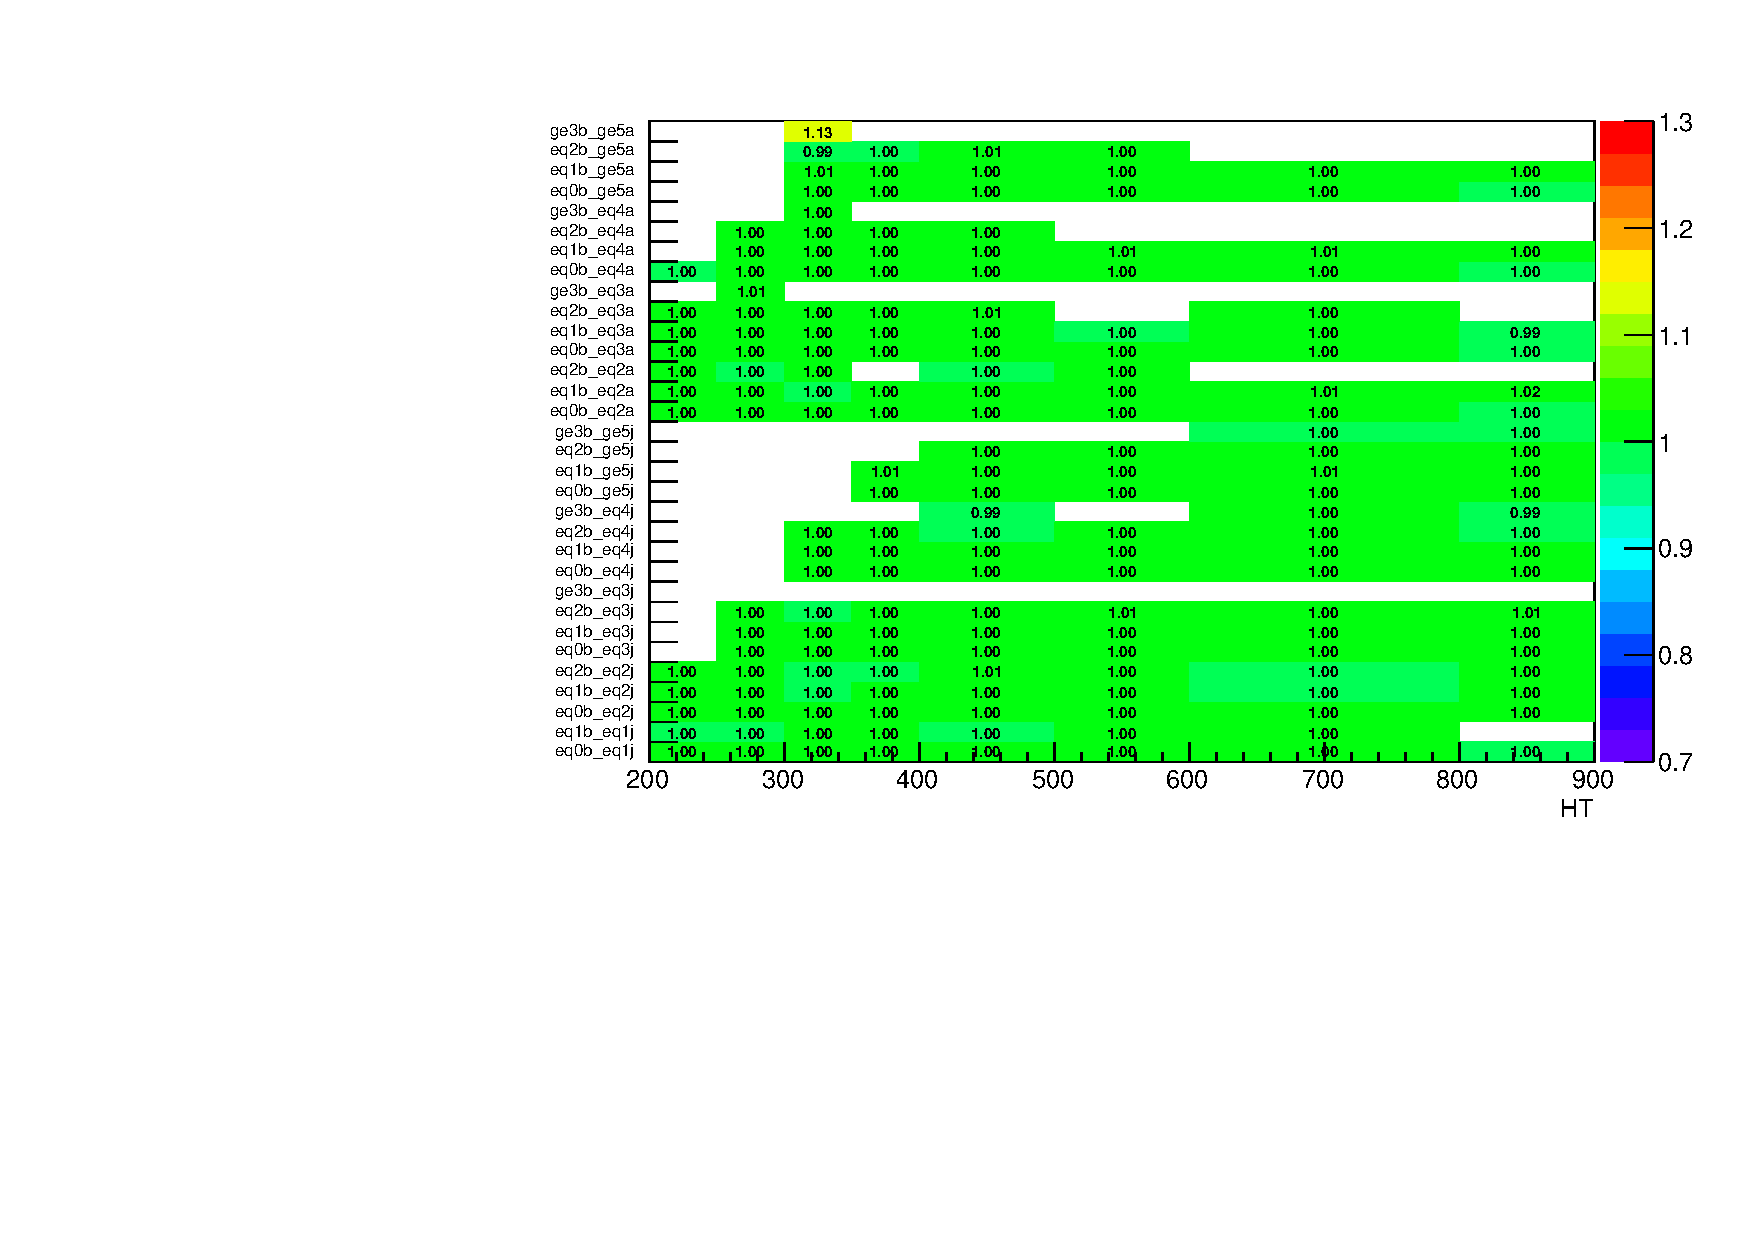
\includegraphics[width=0.5\textwidth]{figs/analysis/systsTf/Zinv/mumu/ratiotfh_ht_mht_allbsfWeight_Up.pdf}
  } ~~
  \subfloat[b-tag SF (heavy) down variation]{
    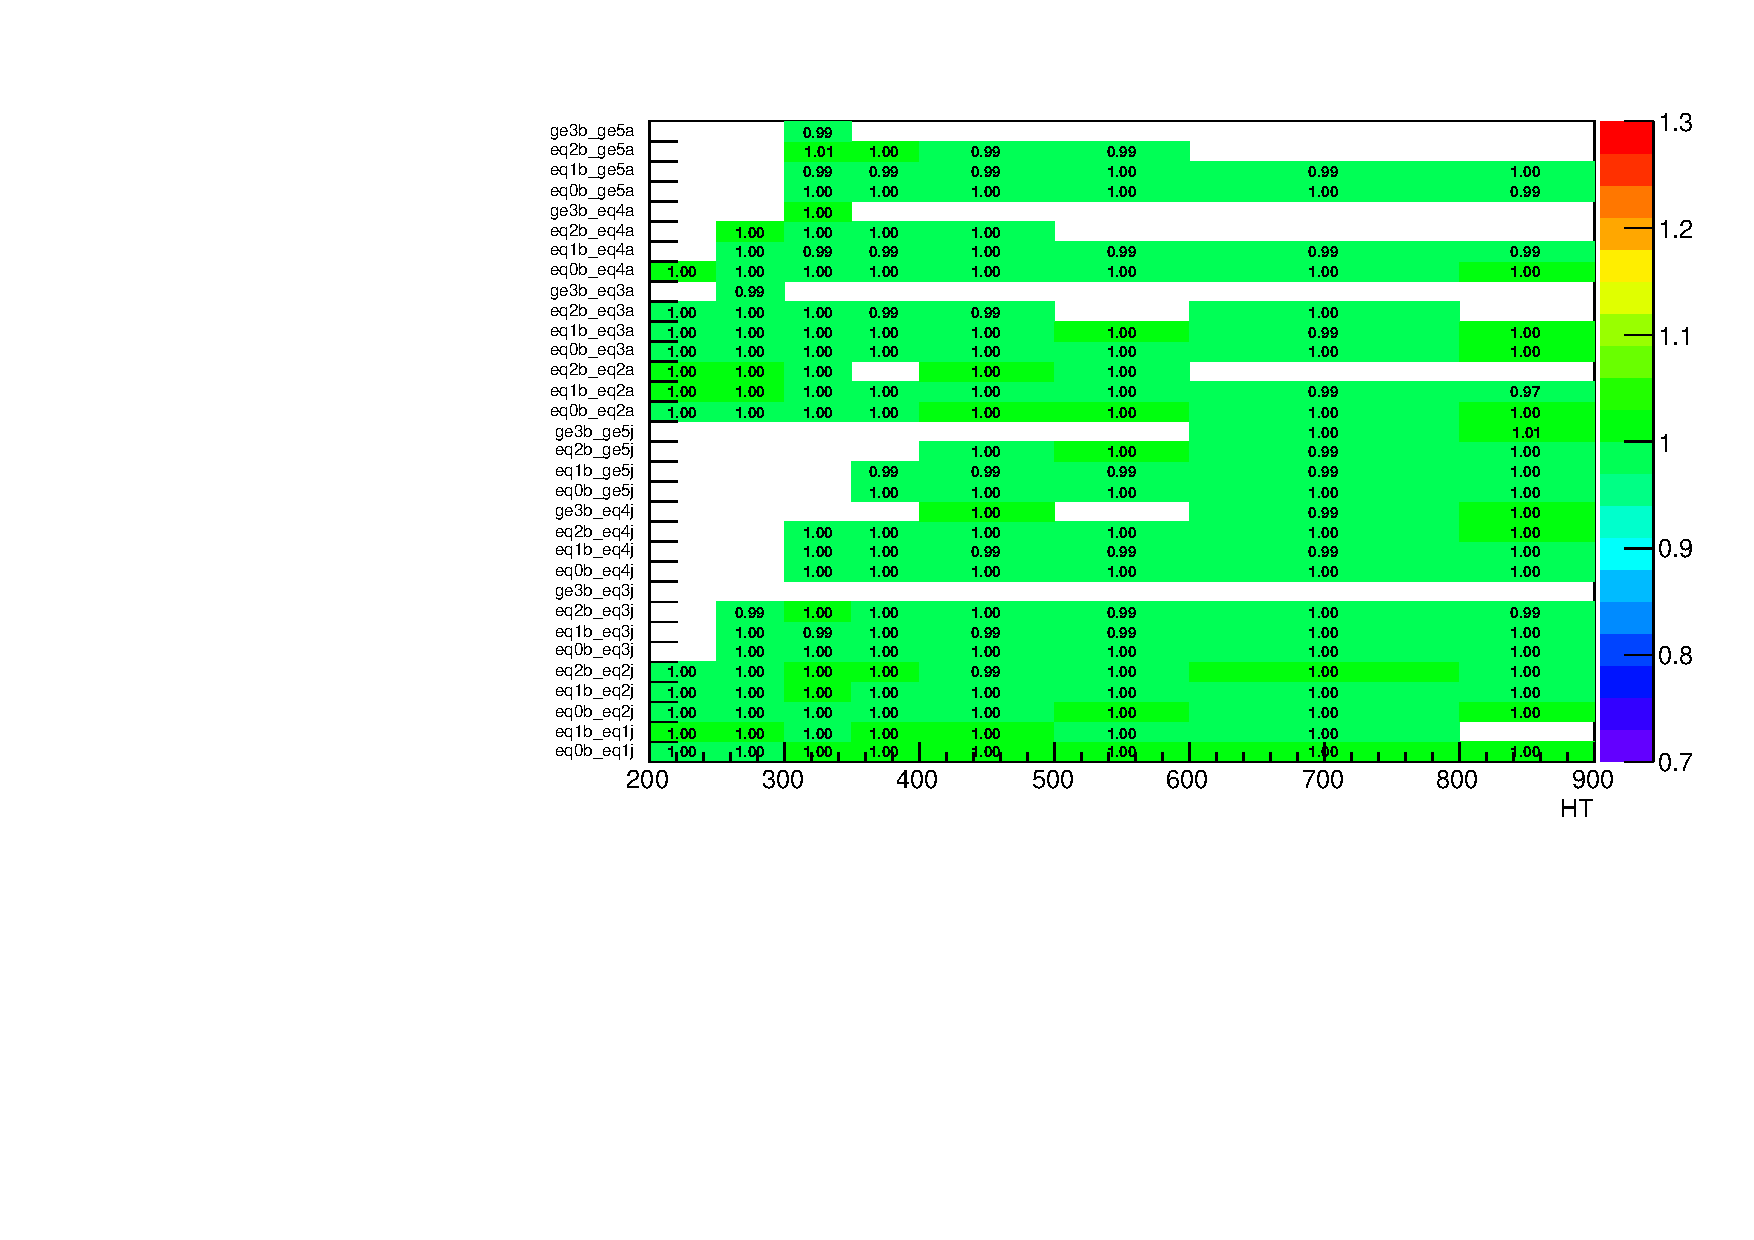
\includegraphics[width=0.5\textwidth]{figs/analysis/systsTf/Zinv/mumu/ratiotfh_ht_mht_allbsfWeight_Down.pdf}
  }\\

  \caption{\label{fig:tfSyst_bsf_mumuToZinv} The relative change in
  the $\mmj \rightarrow (\znunu)$ transfer
  factors when varying b-tag SF for heavy jets in MC within its uncertainties, as a function of \scalht and jet category. 
  Variations corresponding to $+1\sigma$ ($-1\sigma$) are shown in the left (right) figure. 
  }
\end{figure}

\begin{figure}[!h]
  \centering
  \subfloat[b-tag SF (heavy) up variation]{
    \includegraphics[width=0.5\textwidth]{figs/analysis/systsTf/Zinv/gj/ratiotfh_ht_mht_allbsfWeight_Up.pdf}
  } ~~
  \subfloat[b-tag SF (heavy) down variation]{
    \includegraphics[width=0.5\textwidth]{figs/analysis/systsTf/Zinv/gj/ratiotfh_ht_mht_allbsfWeight_Down.pdf}
  }\\

  \caption{\label{fig:tfSyst_bsf_gjToZinv} The relative change in the
  $\gj \rightarrow (\znunu)$ transfer
  factors when varying b-tag SF for heavy jets in MC within its uncertainties, as a function of \scalht and jet category. 
  Variations corresponding to $+1\sigma$ ($-1\sigma$) are shown in the left (right) figure. 
  }
\end{figure}

\begin{figure}[!h]
  \centering
  \subfloat[b-tag SF (heavy) up variation]{
    \includegraphics[width=0.5\textwidth]{figs/analysis/systsTf/Ttw/mu/ratiotfh_ht_mht_allbsfWeight_Up.pdf}
  } ~~
  \subfloat[b-tag SF (heavy) down variation]{
    \includegraphics[width=0.5\textwidth]{figs/analysis/systsTf/Ttw/mu/ratiotfh_ht_mht_allbsfWeight_Down.pdf}
  }\\

  \caption{\label{fig:tfSyst_bsf_muToTtw} The relative change in the $\mj \rightarrow \mathrm{tt+W}$ transfer
  factors when varying b-tag SF for heavy jets in MC within its uncertainties, as a function of \scalht and jet category. 
  Variations corresponding to $+1\sigma$ ($-1\sigma$) are shown in the left (right) figure. 
  }
\end{figure}

\clearpage % too many figures, latex doesn't like it

\begin{figure}[!h]
  \centering
  \subfloat[b-tag SF (light) up variation]{
    \includegraphics[width=0.5\textwidth]{figs/analysis/systsTf/Zinv/mu/ratiotfh_ht_mht_allbsfLightWeight_Up.pdf}
  } ~~
  \subfloat[b-tag SF (light) down variation]{
    \includegraphics[width=0.5\textwidth]{figs/analysis/systsTf/Zinv/mu/ratiotfh_ht_mht_allbsfLightWeight_Down.pdf}
  }\\

  \caption{\label{fig:tfSyst_bsfl_muToZinv} The relative change in the
  $\mj \rightarrow (\znunu)$ transfer
  factors when varying b-tag SF for light jets in MC within its uncertainties, as a function of \scalht and jet category. 
  Variations corresponding to $+1\sigma$ ($-1\sigma$) are shown in the left (right) figure. 
  }
\end{figure}

\begin{figure}[!h]
  \centering
  \subfloat[b-tag SF (light) up variation]{
    \includegraphics[width=0.5\textwidth]{figs/analysis/systsTf/Zinv/mumu/ratiotfh_ht_mht_allbsfLightWeight_Up.pdf}
  } ~~
  \subfloat[b-tag SF (light) down variation]{
    \includegraphics[width=0.5\textwidth]{figs/analysis/systsTf/Zinv/mumu/ratiotfh_ht_mht_allbsfLightWeight_Down.pdf}
  }\\

  \caption{\label{fig:tfSyst_bsfl_mumuToZinv} The relative change in
  the $\mmj \rightarrow (\znunu)$ transfer
  factors when varying b-tag SF for light jets in MC within its uncertainties, as a function of \scalht and jet category. 
  Variations corresponding to $+1\sigma$ ($-1\sigma$) are shown in the left (right) figure. 
  }
\end{figure}

\begin{figure}[!h]
  \centering
  \subfloat[b-tag SF (light) up variation]{
    \includegraphics[width=0.5\textwidth]{figs/analysis/systsTf/Zinv/gj/ratiotfh_ht_mht_allbsfLightWeight_Up.pdf}
  } ~~
  \subfloat[b-tag SF (light) down variation]{
    \includegraphics[width=0.5\textwidth]{figs/analysis/systsTf/Zinv/gj/ratiotfh_ht_mht_allbsfLightWeight_Down.pdf}
  }\\

  \caption{\label{fig:tfSyst_bsfl_gjToZinv} The relative change in the
  $\gj \rightarrow (\znunu)$ transfer
  factors when varying b-tag SF for light jets in MC within its uncertainties, as a function of \scalht and jet category. 
  Variations corresponding to $+1\sigma$ ($-1\sigma$) are shown in the left (right) figure. 
  }
\end{figure}

\begin{figure}[!h]
  \centering
  \subfloat[b-tag SF (light) up variation]{
    \includegraphics[width=0.5\textwidth]{figs/analysis/systsTf/Ttw/mu/ratiotfh_ht_mht_allbsfLightWeight_Up.pdf}
  } ~~
  \subfloat[b-tag SF (light) down variation]{
    \includegraphics[width=0.5\textwidth]{figs/analysis/systsTf/Ttw/mu/ratiotfh_ht_mht_allbsfLightWeight_Down.pdf}
  }\\

  \caption{\label{fig:tfSyst_bsfl_muToTtw} The relative change in the $\mj \rightarrow \mathrm{tt+W}$ transfer
  factors when varying b-tag SF for light jets in MC within its uncertainties, as a function of \scalht and jet category. 
  Variations corresponding to $+1\sigma$ ($-1\sigma$) are shown in the left (right) figure. 
  }
\end{figure}



\begin{figure}[!h]
  \centering
  \subfloat[muon scale factor up variation]{
    \includegraphics[width=0.5\textwidth]{figs/analysis/systsTf/Zinv/mu/ratiotfh_ht_mht_allmuonSfWeight_Up.pdf}
  } ~~
  \subfloat[muon scale factor down variation]{
    \includegraphics[width=0.5\textwidth]{figs/analysis/systsTf/Zinv/mu/ratiotfh_ht_mht_allmuonSfWeight_Down.pdf}
  }\\

  \caption{\label{fig:tfSyst_muon scale factor_muToZinv} The relative change in
  the $\mj \rightarrow (\znunu)$ transfer
  factors when varying muon scale factor in MC within its uncertainties, as a function of \scalht and jet category. 
  Variations corresponding to $+1\sigma$ ($-1\sigma$) are shown in the left (right) figure. 
  }
\end{figure}
\begin{figure}[!h]
  \centering
  \subfloat[muon scale factor up variation]{
    \includegraphics[width=0.5\textwidth]{figs/analysis/systsTf/Zinv/mumu/ratiotfh_ht_mht_allmuonSfWeight_Up.pdf}
  } ~~
  \subfloat[muon scale factor down variation]{
    \includegraphics[width=0.5\textwidth]{figs/analysis/systsTf/Zinv/mumu/ratiotfh_ht_mht_allmuonSfWeight_Down.pdf}
  }\\

  \caption{\label{fig:tfSyst_muon scale factor_mumuToZinv} The relative change in
  the $\mmj \rightarrow (\znunu)$ transfer
  factors when varying muon scale factor in MC within its uncertainties, as a function of \scalht and jet category. 
  Variations corresponding to $+1\sigma$ ($-1\sigma$) are shown in the left (right) figure. 
  }
\end{figure}


\begin{figure}[!h]
  \centering
  \subfloat[muon scale factor up variation]{
    \includegraphics[width=0.5\textwidth]{figs/analysis/systsTf/Ttw/mu/ratiotfh_ht_mht_allmuonSfWeight_Up.pdf}
  } ~~
  \subfloat[muon scale factor down variation]{
    \includegraphics[width=0.5\textwidth]{figs/analysis/systsTf/Ttw/mu/ratiotfh_ht_mht_allmuonSfWeight_Down.pdf}
  }\\

  \caption{\label{fig:tfSyst_muon scale factor_muToTtw} The relative change in the $\mj \rightarrow \mathrm{tt+W}$ transfer
  factors when varying muon scale factor in MC within its uncertainties, as a function of \scalht and jet category. 
  Variations corresponding to $+1\sigma$ ($-1\sigma$) are shown in the left (right) figure. 
  }
\end{figure}
\begin{figure}[!h]
  \centering
  \subfloat[Photon trigger weight up variation]{
    \includegraphics[width=0.5\textwidth]{figs/analysis/systsTf/Zinv/gj/ratiotfh_ht_mht_allphotonTriggerWeight_Up.pdf}
  } ~~
  \subfloat[Photon trigger weight down variation]{
    \includegraphics[width=0.5\textwidth]{figs/analysis/systsTf/Zinv/gj/ratiotfh_ht_mht_allphotonTriggerWeight_Down.pdf}
  }\\

  \caption{\label{fig:tfSyst_photonTrigger_gjToZinv} The relative change in
  the $\gj \rightarrow (\znunu)$ transfer
  factors when varying photon trigger weight in MC within its uncertainties, as a function of \scalht and jet category. 
  Variations corresponding to $+1\sigma$ ($-1\sigma$) are shown in the left (right) figure. 
  }
\end{figure}



\begin{figure}[!h]
  \centering
  \subfloat[trigger weight up variation]{
    \includegraphics[width=0.5\textwidth]{figs/analysis/systsTf/Zinv/mu/ratiotfh_ht_mht_alltriggerWeight_Up.pdf}
  } ~~
  \subfloat[trigger weight down variation]{
    \includegraphics[width=0.5\textwidth]{figs/analysis/systsTf/Zinv/mu/ratiotfh_ht_mht_alltriggerWeight_Down.pdf}
  }\\

  \caption{\label{fig:tfSyst_trigger_muToZinv} The relative change in
  the $\mj \rightarrow (\znunu)$ transfer
  factors when varying trigger weight in MC within its uncertainties, as a function of \scalht and jet category. 
  Variations corresponding to $+1\sigma$ ($-1\sigma$) are shown in the left (right) figure. 
  }
\end{figure}
\begin{figure}[!h]
  \centering
  \subfloat[trigger weight up variation]{
    \includegraphics[width=0.5\textwidth]{figs/analysis/systsTf/Zinv/mumu/ratiotfh_ht_mht_alltriggerWeight_Up.pdf}
  } ~~
  \subfloat[trigger weight down variation]{
    \includegraphics[width=0.5\textwidth]{figs/analysis/systsTf/Zinv/mumu/ratiotfh_ht_mht_alltriggerWeight_Down.pdf}
  }\\

  \caption{\label{fig:tfSyst_trigger_mumuToZinv} The relative change in
  the $\mmj \rightarrow (\znunu)$ transfer
  factors when varying trigger weight in MC within its uncertainties, as a function of \scalht and jet category. 
  Variations corresponding to $+1\sigma$ ($-1\sigma$) are shown in the left (right) figure. 
  }
\end{figure}

\begin{figure}[!h]
  \centering
  \subfloat[trigger weight up variation]{
    \includegraphics[width=0.5\textwidth]{figs/analysis/systsTf/Zinv/gj/ratiotfh_ht_mht_alltriggerWeight_Up.pdf}
  } ~~
  \subfloat[trigger weight down variation]{
    \includegraphics[width=0.5\textwidth]{figs/analysis/systsTf/Zinv/gj/ratiotfh_ht_mht_alltriggerWeight_Down.pdf}
  }\\

  \caption{\label{fig:tfSyst_trigger_gjToZinv} The relative change in
  the $\gj \rightarrow (\znunu)$ transfer
  factors when varying trigger weight in MC within its uncertainties, as a function of \scalht and jet category. 
  Variations corresponding to $+1\sigma$ ($-1\sigma$) are shown in the left (right) figure. 
  }
\end{figure}

\begin{figure}[!h]
  \centering
  \subfloat[trigger weight up variation]{
    \includegraphics[width=0.5\textwidth]{figs/analysis/systsTf/Ttw/mu/ratiotfh_ht_mht_alltriggerWeight_Up.pdf}
  } ~~
  \subfloat[trigger weight down variation]{
    \includegraphics[width=0.5\textwidth]{figs/analysis/systsTf/Ttw/mu/ratiotfh_ht_mht_alltriggerWeight_Down.pdf}
  }\\

  \caption{\label{fig:tfSyst_trigger_muToTtw} The relative change in the $\mj \rightarrow \mathrm{tt+W}$ transfer
  factors when varying trigger weight in MC within its uncertainties, as a function of \scalht and jet category. 
  Variations corresponding to $+1\sigma$ ($-1\sigma$) are shown in the left (right) figure. 
  }
\end{figure}

\begin{figure}[!h]
  \centering
  \subfloat[top $p_{T}$ weight up variation]{
    \includegraphics[width=0.5\textwidth]{figs/analysis/systsTf/Zinv/mu/ratiotfh_ht_mht_alltopPtWeight_Up.pdf}
  } ~~
  \subfloat[top $p_{T}$ weight down variation]{
    \includegraphics[width=0.5\textwidth]{figs/analysis/systsTf/Zinv/mu/ratiotfh_ht_mht_alltopPtWeight_Down.pdf}
  }\\

  \caption{\label{fig:tfSyst_topPt_muToZinv} The relative change in
  the $\mj \rightarrow (\znunu)$ transfer
  factors when varying top $p_{T}$ weight in MC within its uncertainties, as a function of \scalht and jet category. 
  Variations corresponding to $+1\sigma$ ($-1\sigma$) are shown in the left (right) figure. 
  }
\end{figure}
\begin{figure}[!h]
  \centering
  \subfloat[top $p_{T}$ weight up variation]{
    \includegraphics[width=0.5\textwidth]{figs/analysis/systsTf/Zinv/mumu/ratiotfh_ht_mht_alltopPtWeight_Up.pdf}
  } ~~
  \subfloat[top $p_{T}$ weight down variation]{
    \includegraphics[width=0.5\textwidth]{figs/analysis/systsTf/Zinv/mumu/ratiotfh_ht_mht_alltopPtWeight_Down.pdf}
  }\\

  \caption{\label{fig:tfSyst_topPt_mumuToZinv} The relative change in
  the $\mmj \rightarrow (\znunu)$ transfer
  factors when varying top $p_{T}$ weight in MC within its uncertainties, as a function of \scalht and jet category. 
  Variations corresponding to $+1\sigma$ ($-1\sigma$) are shown in the left (right) figure. 
  }
\end{figure}

\begin{figure}[!h]
  \centering
  \subfloat[top $p_{T}$ weight up variation]{
    \includegraphics[width=0.5\textwidth]{figs/analysis/systsTf/Ttw/mu/ratiotfh_ht_mht_alltopPtWeight_Up.pdf}
  } ~~
  \subfloat[top $p_{T}$ weight down variation]{
    \includegraphics[width=0.5\textwidth]{figs/analysis/systsTf/Ttw/mu/ratiotfh_ht_mht_alltopPtWeight_Down.pdf}
  }\\

  \caption{\label{fig:tfSyst_topPt_muToTtw} The relative change in the $\mj \rightarrow \mathrm{tt+W}$ transfer
  factors when varying top $p_{T}$ weight in MC within its uncertainties, as a function of \scalht and jet category. 
  Variations corresponding to $+1\sigma$ ($-1\sigma$) are shown in the left (right) figure. 
  }
\end{figure}



\begin{figure}[!h]
  \centering
  \subfloat[PU weight up variation]{
    \includegraphics[width=0.5\textwidth]{figs/analysis/systsTf/Zinv/mu/ratiotfh_ht_mht_allpuWeight_Up.pdf}
  } ~~
  \subfloat[PU weight down variation]{
    \includegraphics[width=0.5\textwidth]{figs/analysis/systsTf/Zinv/mu/ratiotfh_ht_mht_allpuWeight_Down.pdf}
  }\\

  \caption{\label{fig:tfSyst_pu_muToZinv} The relative change in the
  $\mj \rightarrow (\znunu)$ transfer
  factors when varying PU weight in MC within its uncertainties, as a function of \scalht and jet category. 
  Variations corresponding to $+1\sigma$ ($-1\sigma$) are shown in the left (right) figure. 
  }
\end{figure}

\begin{figure}[!h]
  \centering
  \subfloat[PU weight up variation]{
    \includegraphics[width=0.5\textwidth]{figs/analysis/systsTf/Zinv/mumu/ratiotfh_ht_mht_allpuWeight_Up.pdf}
  } ~~
  \subfloat[PU weight down variation]{
    \includegraphics[width=0.5\textwidth]{figs/analysis/systsTf/Zinv/mumu/ratiotfh_ht_mht_allpuWeight_Down.pdf}
  }\\

  \caption{\label{fig:tfSyst_pu_mumuToZinv} The relative change in the
  $\mmj \rightarrow (\znunu)$ transfer
  factors when varying PU weight in MC within its uncertainties, as a function of \scalht and jet category. 
  Variations corresponding to $+1\sigma$ ($-1\sigma$) are shown in the left (right) figure. 
  }
\end{figure}

\begin{figure}[!h]
  \centering
  \subfloat[PU weight up variation]{
    \includegraphics[width=0.5\textwidth]{figs/analysis/systsTf/Zinv/gj/ratiotfh_ht_mht_allpuWeight_Up.pdf}
  } ~~
  \subfloat[PU weight down variation]{
    \includegraphics[width=0.5\textwidth]{figs/analysis/systsTf/Zinv/gj/ratiotfh_ht_mht_allpuWeight_Down.pdf}
  }\\

  \caption{\label{fig:tfSyst_pu_gjToZinv} The relative change in the
  $\gj \rightarrow (\znunu)$ transfer
  factors when varying PU weight in MC within its uncertainties, as a function of \scalht and jet category. 
  Variations corresponding to $+1\sigma$ ($-1\sigma$) are shown in the left (right) figure. 
  }
\end{figure}

\begin{figure}[!h]
  \centering
  \subfloat[PU weight up variation]{
    \includegraphics[width=0.5\textwidth]{figs/analysis/systsTf/Ttw/mu/ratiotfh_ht_mht_allpuWeight_Up.pdf}
  } ~~
  \subfloat[PU weight down variation]{
    \includegraphics[width=0.5\textwidth]{figs/analysis/systsTf/Ttw/mu/ratiotfh_ht_mht_allpuWeight_Down.pdf}
  }\\

  \caption{\label{fig:tfSyst_pu_muToTtw} The relative change in the $\mj \rightarrow \mathrm{tt+W}$ transfer
  factors when varying PU weight in MC within its uncertainties, as a function of \scalht and jet category. 
  Variations corresponding to $+1\sigma$ ($-1\sigma$) are shown in the left (right) figure. 
  }
\end{figure}



